%%%%%%%%%%%%%%%%%%%%%%%%%%%%%%%%%%%%%%%%%
% Modelo trabalho de conclusão de curso
% Bacharelado em Sistemas de Informação - IFNMG - Campus Salinas
% Version 2 (1º semestre 2021)
%
% Modelo adaptado de:
% Frits Wenneker (http://www.howtotex.com)
%
% License:
% CC BY-NC-SA 3.0 (http://creativecommons.org/licenses/by-nc-sa/3.0/)
%
% Texto adaptado de: http://www.fea.usp.br/media/fck/File/Roteiro_para_projeto_pesquisa.pdf
%%%%%%%%%%%%%%%%%%%%%%%%%%%%%%%%%%%%%%%%%


\documentclass[
	% -- opções da classe memoir --
	12pt,				% tamanho da fonte
	%openright,			% capítulos começam em pág ímpar (insere página vazia caso preciso)
	twoside,			% para impressão em recto e verso. Oposto a oneside
	a4paper,			% tamanho do papel.
	% -- opções da classe abntex2 --
	chapter=TITLE,		% títulos de capítulos convertidos em letras maiúsculas
	section=TITLE,		% títulos de seções convertidos em letras maiúsculas
	subsection=TITLE,	% títulos de subseções convertidos em letras maiúsculas
	subsubsection=TITLE,% títulos de subsubseções convertidos em letras maiúsculas
	% -- opções do pacote babel --
	english,			% idioma adicional para hifenização
	french,				% idioma adicional para hifenização
	spanish,			% idioma adicional para hifenização
	brazil,				% o último idioma é o principal do documento
	]{abntex2}

% ---------------------------------
% PACOTES
% ---------------------------------
%\renewcommand{\thesection}{\arabic{section}}
\usepackage{lmodern}			% Usa a fonte Latin Modern
\usepackage[T1]{fontenc}		% Selecao de codigos de fonte.
\usepackage[utf8]{inputenc}		% Codificacao do documento (conversão automática dos acentos)
\usepackage{indentfirst}		% Indenta o primeiro parágrafo de cada seção.
\usepackage{color}				% Controle das cores
\usepackage{lastpage}
\usepackage{graphicx}			% Inclusão de gráficos
\usepackage{microtype} 			% para melhorias de justificação
\usepackage{multirow}
\usepackage{amsmath,amsfonts,amssymb}
\usepackage[table]{xcolor}
\usepackage{multirow}           % Merge rows and columns in tables
\usepackage{longtable}          % Large tables
\usepackage{fancyvrb}           % Codes and Outputs commands
\usepackage{listings}           % Codes and Outputs commands
\usepackage{pdflscape}
\usepackage{float}
\usepackage{subfig}             % Subfigures
\usepackage{latexsym}           % Extra symbols of Latex
\usepackage{booktabs}
\usepackage{enumerate}
\usepackage{acronym}
\usepackage[portuguese, ruled, linesnumbered]{algorithm2e}
\usepackage[noend]{algpseudocode}
\usepackage{url}
\let\realurl\url
\renewcommand{\url}[1]{\realurl{#1}\wlog{URLX #1}}
\usepackage{lipsum}				% To generate dummy text

% ---------------------------------
% Pacotes de citações
% ---------------------------------
\usepackage[brazilian,hyperpageref]{backref}% Paginas com as citações na bibl
\usepackage[alf,bibjustif]{abntex2cite}	% Citações padrão ABNT

% ---------------------------------
% Configurações do pacote backref
% Usado sem a opção hyperpageref de backref
\renewcommand{\backrefpagesname}{Citado na(s) página(s):~}
% Texto padrão antes do número das páginas
\renewcommand{\backref}{}
% Define os textos da citação
\renewcommand*{\backrefalt}[4]{
	\ifcase #1 %
		Nenhuma citação no texto.%
	\or
		Citado na página #2.%
	\else
		Citado #1 vezes nas páginas #2.%
	\fi}%
% ---------------------------------
% Configurações de aparência do PDF final
% ---------------------------------
% alterando o aspecto da cor azul
\definecolor{blue}{RGB}{41,5,195}

% informações do PDF
\makeatletter
\hypersetup{
     	%pagebackref=true,
		pdftitle={\@title},
		pdfauthor={\@author},
    	pdfsubject={\imprimirpreambulo},
	    pdfcreator={LaTeX with abnTeX2},
		pdfkeywords={abnt}{latex}{abntex}{abntex2}{projeto de pesquisa},
		colorlinks=true,       		% false: boxed links; true: colored links
    	linkcolor=blue,          	% color of internal links
    	citecolor=blue,        		% color of links to bibliography
    	filecolor=magenta,      		% color of file links
		urlcolor=blue,
		bookmarksdepth=4
}
\makeatother
% ---------------------------------
% Espaçamentos entre linhas e parágrafos
% ---------------------------------
% O tamanho do parágrafo é dado por:
\setlength{\parindent}{1.3cm}
% Controle do espaçamento entre um parágrafo e outro:
\setlength{\parskip}{0.2cm}  % tente também \onelineskip


%-----------------------------------
% Front pages
%-----------------------------------
\titulo{Plataforma Web para Exibição de Horários Acadêmicos no IFNMG - Campus Salinas}
\autor{Tomaz Martins Batista}
\local{Salinas - Minas Gerais}
\date{\normalsize\today} % Gera automaticamente a data
\orientador{Leonardo Humberto Guimarães Silva}
\instituicao{%
 	Instituto Federal do Norte de Minas Gerais - Campus Salinas
 	\par  
 	Bacharelado em Sistemas de Informação
}

\preambulo{Trabalho de conclusão de curso apresentado ao Curso de Bacharelado em Sistemas de Informação do Instituto Federal do Norte de Minas Gerais, como exigência para obtenção do grau de Bacharel em Sistemas de Informação.}

%-----------------------------------
% Set the final PDF
%-----------------------------------
\definecolor{blue}{RGB}{41,5,195} % setting the blue color

% PDF informations
\makeatletter                   
\hypersetup{
     	%pagebackref=true,
		pdftitle={\@title}, 
		pdfauthor={\@author},
    	pdfsubject={\imprimirpreambulo},
	    pdfcreator={LaTeX with abnTeX2},
		pdfkeywords={abnt}{latex}{abntex}{abntex2}{trabalho acadêmico}, 
		colorlinks=true,        % false: boxed links; true: colored links
    	linkcolor=blue,         % color of internal links
    	citecolor=blue,        	% color of links to bibliography
    	filecolor=magenta,      % color of file links
		urlcolor=blue,
		bookmarksdepth=4
}
\makeatother

%-----------------------------------
% Spacing between lines and paragraphs
%-----------------------------------
\setlength{\parindent}{1.5cm}   % Set length of indent
\setlength{\parskip}{0.2cm}     % Set length among the paragraphs 

%Index
\makeindex

%-----------------------------------
% Main document
%-----------------------------------
\begin{document}

%-----------------------------------
% Linguagem
\selectlanguage{brazil} % Texts in pt-br
\frenchspacing          % Remove obsolete spaces between phrases

%-----------------------------------
% Elementos pre-textuais
\pretextual

%-----------------------------------
% Capa
\imprimircapa                   

% Folha de rosto
\imprimirfolhaderosto

\newpage

%-----------------------------------
% Dedicatória (opcional)
\begin{dedicatoria}
   \vspace*{\fill}
   \centering
   \noindent
   \textit{Dedico este trabalho à minha família, aos amigos, aos professores e a todos que me apoiaram ao longo do curso.}
   \vspace*{\fill}
\end{dedicatoria}

%-----------------------------------
% Agradecimentos (opcional)
\begin{agradecimentos}

Antes de tudo, agradeço a Deus, que me sustentou em cada etapa desta jornada, concedendo força, sabedoria e perseverança para superar desafios e alcançar meus objetivos.

À minha família, expresso minha mais profunda gratidão pelo amor incondicional, pelo apoio constante e por sempre acreditarem no meu potencial, mesmo nos momentos mais difíceis.

Expresso minha gratidão aos colegas de curso pela parceria, pelo compartilhamento de ideias e pelo apoio ao longo das atividades, que contribuíram significativamente para minha formação.

Agradeço, de modo especial, ao professor Leonardo pela orientação durante o desenvolvimento deste trabalho e por compartilhar seus conhecimentos sobre desenvolvimento web.

Estendo também meu agradecimento especial ao professor Frederico, pela orientação durante o período da bolsa treinamento e pelas contribuições no entendimento da gestão dos horários acadêmicos do IFNMG - Campus Salinas.

\end{agradecimentos}

%-----------------------------------
% Resumo (em português)
\setlength{\absparsep}{18pt} % set spacing between the paragraphs

\begin{resumo}
	O presente trabalho teve como objetivo facilitar a exibição dos horários acadêmicos do IFNMG - Campus Salinas, tornando o acesso mais intuitivo, seguro e eficiente, em atendimento às demandas do setor de ensino. A pesquisa partiu do problema identificado no uso de planilhas do \textit{Google Sheets}, devido a falhas de segurança e limitações de usabilidade, especialmente em dispositivos móveis e na busca por informações específicas. Para alcançar o objetivo proposto, foi adotada a metodologia de desenvolvimento de um sistema que integra tecnologias modernas, como \textit{Next.js}, \textit{Tailwind CSS} e \textit{Spring Boot}, mantendo o \textit{Google Sheets} como banco de dados. A implantação foi seguida por um processo de avaliação para ajustes e melhorias. Os principais resultados incluem a criação de telas específicas para cursos, professores e salas, a implementação de uma tela de validação de dados com acesso restrito e a elaboração de uma documentação técnica da planilha. Por fim, a solução desenvolvida aumentou a confiabilidade, a acessibilidade e a organização dos dados, além de apresentar uma abordagem alternativa de banco de dados para sistemas web.
    
    Palavras-chave: Desenvolvimento Web, Plataforma Web, Horários Acadêmicos,
	\textit{Next.js}, \textit{Spring Boot}, \textit{Google Sheets}.
\end{resumo}

%-----------------------------------
% Abstract (in English) (opcional)
\begin{resumo}[Abstract]
    \begin{otherlanguage*}{english}
        The present work aimed to facilitate the display of academic schedules of IFNMG – Campus Salinas, making access more intuitive, secure, and efficient, in response to the demands of the academic affairs department. The research originated from the problem identified in the use of \textit{Google Sheets} spreadsheets, due to security flaws and usability limitations, especially on mobile devices and in the search for specific information. To achieve the proposed objective, a system development methodology was adopted that integrates modern technologies such as \textit{Next.js}, \textit{Tailwind CSS}, and \textit{Spring Boot}, while maintaining \textit{Google Sheets} as the database. The implementation was followed by an evaluation process for adjustments and improvements. The main results include the creation of specific screens for courses, teachers, and classrooms, the implementation of a data validation screen with restricted access, and the preparation of technical documentation for the spreadsheet. Finally, the developed solution increased the reliability, accessibility, and organization of the data, in addition to presenting an alternative database approach for web systems.

        \textit{Keywords: Web Development, Web Platform, Academic Schedules, Next.js, Spring Boot, Google Sheets.}
    \end{otherlanguage*}
\end{resumo}

%-----------------------------------
% Lista de figuras
\pdfbookmark[0]{\listfigurename}{lof}
\listoffigures*
\cleardoublepage

%-----------------------------------
% Abreviações (opcional)
%-----------------------------------
% Abbreviations and acronyms
%-----------------------------------

\begin{siglas}
  \item[IFNMG] Instituto Federal do Norte de Minas Gerais
  \item[SSR] Server-Side Rendering
  \item[CSR] Client-Side Rendering
  \item[SSG] Static Site Generation
  \item[ISR] Incremental Static Regeneration
  \item[CSS] Cascading Style Sheets
  \item[HTML] HyperText Markup Language
  \item[SGBD] Sistema de Gerenciamento de Banco de Dados
  \item[JVM] Java Virtual Machine
  \item[API] Application Programming Interface
  \item[MVC] Model-View-Controller
  \item[HTTP] Hypertext Transfer Protocol
  \item[REST] Representational State Transfer
  \item[JSON] JavaScript Object Notation
  \item[CORS] Cross-Origin Resource Sharing
\end{siglas}
\cleardoublepage

%-----------------------------------
% Sumário
\pdfbookmark[0]{\contentsname}{toc}
\tableofcontents*
\cleardoublepage


%-----------------------------------
% TEXTUAL ELEMENTS
%-----------------------------------
\textual

%-----------------------------------
% Chapters
\chapter{Introdução} 
\label{cap1_introducao} 

Todos os departamentos de ensino enfrentam, no início de cada semestre acadêmico, a necessidade de criar horários escolares. A elaboração de um horário acadêmico é uma tarefa complexa, que envolve a gestão de restrições entre alunos, professores e salas em determinados períodos letivos, e deve ser apoiada por sistemas de informação avançados. A combinação de sistemas capazes de gerenciar informações acadêmicas e técnicas de pesquisa e otimização eficientes pode possibilitar a geração semiautomática de horários acadêmicos, com um desempenho que, na maioria das vezes, seria difícil de alcançar com um processo tradicional, essencialmente manual \cite{passos2016}.

O IFNMG - Campus Salinas é uma instituição pública de ensino que se destaca em oferecer educação profissional e tecnológica em diversos níveis, do ensino médio ao superior \cite{ifnmgsalinas2014}. Nos ambientes acadêmicos, a gestão de horários desempenha um papel central na organização das atividades, sendo essencial para o bom funcionamento de instituições de ensino. A eficiência no acesso a essas informações, tanto para alunos quanto para servidores, impacta diretamente a rotina acadêmica e administrativa \cite{Urania2024}. Entretanto, em muitas instituições, como o IFNMG - Campus Salinas, a organização dos horários é realizada por meio de planilhas. Embora amplamente utilizadas, apresentam limitações que dificultam a consulta, a manutenção e a proteção das informações, criando um cenário desafiador para a administração acadêmica.

A transformação digital, cada vez mais presente no setor educacional, demonstra que informatizar processos administrativos deixou de ser uma conveniência para se tornar uma estratégia essencial. Em ambientes acadêmicos, o uso de plataformas digitais não apenas melhora a eficiência, como também otimiza a gestão de informações críticas \cite{Educacional2023}. De acordo com o Coordenador de Ensino Superior/Diretor de Ensino Substituto do Campus Salinas:

\begin{citacao}
Além da confecção dos horários, que se mostra sempre desafiadora, a apresentação da planilha à comunidade acadêmica e sua manutenção têm se tornado cada vez mais difíceis. A necessidade de permitir que usuários visualizem os horários de forma clara é prejudicada pelas restrições da planilha em uso. Com design pouco intuitivo, falta de responsividade em dispositivos móveis e dificuldade na busca por horários de um curso específico. Tais limitações deixam claro que a modernização do sistema de exibição de horários é fundamental para garantir maior eficiência e acessibilidade.
\end{citacao}

Antes da proposta deste trabalho, a organização dos horários acadêmicos no IFNMG - Campus Salinas era realizada por meio de uma planilha no Google Sheets. O acesso era compartilhado com todos os usuários da instituição por meio de um link aberto, configurado originalmente apenas para visualização. No entanto, foram relatados problemas recorrentes de segurança, nos quais algumas pessoas conseguiam realizar edições indevidas, mesmo sem autorização para isso. Tais falhas comprometiam a integridade dos dados e exigiam intervenções constantes da equipe responsável.

Embora a estrutura da planilha atendesse minimamente à função proposta, apresentava limitações significativas de usabilidade, especialmente na visualização em dispositivos móveis e na busca por informações específicas, como horários por curso. A ausência de uma plataforma dedicada para gerenciar essas informações tornava o processo vulnerável e pouco eficiente.

Tendo isso em vista, o presente trabalho propõe uma solução em formato de plataforma web, com o potencial de otimizar a gestão dos horários acadêmicos no IFNMG - Campus Salinas. Com uma interface intuitiva e mais segura, o sistema facilita a consulta e a visualização das informações, ao mesmo tempo em que impede alterações não autorizadas, garantindo a integridade dos dados. Dessa forma, o setor de ensino poderá gerenciar as informações de forma mais eficiente, sem precisar refazer processos ou depender de bancos de dados complexos.

Por fim, a metodologia do trabalho é baseada no desenvolvimento de um sistema que integra tecnologias modernas para exibição dos horários acadêmicos. Durante o processo, foram realizadas etapas como levantamento de requisitos, prototipação da interface e implementação do sistema. A solução foi desenvolvida utilizando \textit{Next.js} para o \textit{front-end}, com integração ao \textit{Tailwind CSS}, enquanto o \textit{back-end} foi construído com \textit{Spring Boot}, garantindo a conexão com o \textit{Google Sheets}, que funciona como banco de dados.

A primeira versão do sistema foi implantada no segundo semestre de 2024 e, desde então, tem sido amplamente utilizado pela comunidade acadêmica do campus. A adoção da plataforma tem demonstrado ganhos significativos em acessibilidade, organização e segurança dos dados, tornando o processo de consulta dos horários mais eficiente e confiável.

Além disso, foi realizada a avaliação da plataforma com os responsáveis pela gestão dos horários acadêmicos, visando coletar feedbacks para ajustes e melhorias. Foram implementadas melhorias e atualizações a partir das sugestões e críticas obtidas durante essa avaliação. Ademais, elaborou-se uma documentação técnica para definir diretrizes sobre elementos cruciais do sistema, assegurando sua continuidade e manutenção.

O presente trabalho está organizado em seis capítulos. No Capítulo \ref{cap2_objetivos}, são definidos o objetivo geral e os objetivos específicos da pesquisa. O Capítulo \ref{cap3_revisao} apresenta a revisão da literatura que embasa o desenvolvimento do trabalho. O Capítulo \ref{cap4_metodologia} descreve a metodologia adotada ao longo do projeto. O Capítulo \ref{cap5_resultados} foca na apresentação e análise dos resultados obtidos. Por fim, o Capítulo \ref{cap6_conclusao} reúne as principais conclusões e reflexões decorrentes do estudo.
\chapter{Objetivos} 
\label{cap2_objetivos} 

\section{Objetivo Geral}

Facilitar a exibição dos horários acadêmicos do IFNMG - Campus Salinas, com o objetivo de tornar o acesso a essas informações mais intuitivo, seguro e eficiente, atendendo às demandas do setor de ensino.

\section{Objetivos Específicos}

\begin{itemize}
    \item Utilizar os conhecimentos adquiridos durante o curso para propor uma solução web simples e funcional, mantendo a planilha como banco de dados.
    \item Avaliar a plataforma com os responsáveis pela gestão dos horários acadêmicos, com base em critérios de usabilidade, eficiência e organização das informações.
    \item Analisar a viabilidade técnica das melhorias propostas, considerando sua relevância para os usuários e o contexto institucional.
    \item Elaborar uma documentação técnica que descreva a estrutura da planilha utilizada como banco de dados, bem como regras e padrões a serem seguidos para a manutenção futura do sistema.
    \item Contribuir com a organização dos horários escolares no IFNMG - Campus Salinas, melhorando o acesso para toda a comunidade escolar.
\end{itemize}
\chapter{Revisão da Literatura} 
\label{cap3_revisao} 

\section{Tecnologias Digitais na Educação}

A adoção das tecnologias digitais e das plataformas de ensino no contexto educacional tem-se consolidado como uma tendência irreversível, trazendo novos desafios e oportunidades para o Ensino Superior. A incorporação dessas ferramentas não apenas enriquece o processo de ensino e aprendizagem, mas também amplia as possibilidades de interação, colaboração e acesso a recursos educacionais diversificados. A implementação dessas tecnologias é especialmente relevante, dado o contexto socioeconômico e as especificidades regionais que influenciam diretamente o cotidiano acadêmico \cite{Ferreira_Lopes_Oliveira_Carvalho_Souza_Santos_Silva_Veloso_2024}.

Segundo \citeonline{Fernandes2020}, as plataformas digitais desempenham um papel fundamental na organização e otimização dos processos educacionais, promovendo maior transparência e eficiência no gerenciamento de dados acadêmicos. Essa transformação é especialmente relevante em áreas como o planejamento acadêmico e a distribuição de recursos, impactando diretamente a organização das atividades diárias e o suporte à tomada de decisões no ambiente educacional.

A implementação de sistemas digitais em instituições acadêmicas enfrenta desafios
significativos, como a resistência à mudança por servidores e alunos. A falta de capacitação e questões de segurança de dados também são críticas, além do custo de manutenção e integração com sistemas existentes \cite{senger2022gestao}. 

No IFNMG - Campus Salinas, a proposta de integrar uma plataforma web à planilha atual busca minimizar esses desafios, combinando inovação com familiaridade. \citeonline{garcia2024plataforma} destaca que essa estratégia reduz resistências, facilita a centralização de informações de forma segura, acessível e agradável de navegar.

\section{Sistemas Web}

A tecnologia é indispensável para modernizar e otimizar a gestão escolar, transformando processos e promovendo uma administração mais eficiente \cite{Urania2024}. No contexto do IFNMG - Campus Salinas, a adoção de um sistema web para a organização e exibição de horários acadêmicos visa superar as limitações apresentadas pelo uso de planilhas tradicionais, promovendo maior acessibilidade, organização e segurança dos dados.

Um sistema web é uma aplicação que pode variar de páginas simples a sites complexos, sendo acessada por meio de navegadores em diferentes dispositivos conectados à internet \cite{pressman2016engenharia}. Essa característica é especialmente útil em instituições de ensino com uma comunidade acadêmica distribuída, facilitando o acesso simultâneo por alunos, professores e servidores. Segundo \citeonline{silveira2015uef}, a demanda por aplicações web visa atender às diversas necessidades das pessoas e organizações, como apoiar a realização de atividades laborais, comerciais, educacionais e de comunicação, entre outras.

Independentemente do processo adotado, o desenvolvimento de uma aplicação web envolve quatro atividades fundamentais. A primeira fase é a especificação de software, onde as funcionalidades e as restrições do sistema devem ser definidas. Em seguida, passa-se para a fase de projeto e implementação de software, onde o sistema deve ser produzido para atender às especificações. Após a implementação, inicia-se a fase de validação de software, onde o sistema deve ser validado para garantir que atenda às demandas do cliente. Por fim, a fase de evolução de software, onde o sistema deve evoluir para atender às necessidades de mudança dos clientes \cite{sommerville2011engenharia}.

\subsection{Levantamento de Requisitos}

O levantamento de requisitos é uma etapa essencial no processo de desenvolvimento de software, pois define as funcionalidades e as restrições do sistema a ser construído \cite{Balieiro_Pinto_2025}.

De acordo com \citeonline{sommerville2011engenharia}, nessa atividade, os engenheiros de software trabalham com clientes e usuários finais do sistema para obter informações sobre o domínio da aplicação, os serviços que o sistema deve oferecer, o desempenho do sistema, restrições de hardware e assim por diante. Os requisitos podem ser classificados como:

\begin{itemize}
    \item \textbf{Funcionais}: Definem os serviços que o sistema deve fornecer, de como deve reagir a entradas específicas e de como deve se comportar em determinadas situações. Em alguns casos, também podem explicitar o que o sistema não deve fazer.
    \item \textbf{Não Funcionais}: Impõem restrições aos serviços ou funções oferecidos pelo sistema. Incluem restrições de timing, restrições no processo de desenvolvimento e restrições impostas pelas normas. Ao contrário dos requisitos funcionais, muitas vezes, aplicam-se ao sistema como um todo.
\end{itemize}

Neste trabalho, será adotada a técnica de entrevistas, que consiste em conversas estruturadas com os responsáveis pelo setor de ensino. Conforme \citeonline{kendall2011systems} em todo o desenvolvimento de software, um aspecto fundamental é a captura dos requisitos dos usuários. Uma entrevista de levantamento de informações é uma conversa direcionada com um propósito específico, que utiliza um formato ``pergunta/resposta''. Durante esse processo, busca-se obter as opiniões do entrevistado, conhecer os sentimentos do entrevistado sobre o estado corrente do sistema, obter metas organizacionais e pessoais, além de levantar procedimentos informais para interação com tecnologias da informação.

Em uma entrevista, o engenheiro de software está, provavelmente, estabelecendo um relacionamento com uma pessoa desconhecida. Para que esse processo seja eficaz, deve seguir três etapas principais:

\begin{itemize}
    \item \textbf{Planejamento}: Definir os objetivos da entrevista, estudar materiais sobre os entrevistados e a organização, preparar perguntas e estruturar a entrevista para garantir que todas as informações essenciais sejam abordadas.
    \item \textbf{Condução}: Realizar a entrevista de forma organizada, registrando as respostas por meio de anotações ou gravações, garantindo que o entrevistado se sinta à vontade e forneça informações relevantes.
    \item \textbf{Elaboração do Relatório}: Documentar os principais pontos discutidos, destacando informações críticas e identificando aspectos que precisam ser aprofundados em entrevistas futuras.
\end{itemize}

\subsection{Front-end}

O front-end é a interface visual de um site com a qual os usuários interagem diretamente. Engloba todos os elementos visuais, como layouts, botões, imagens, além da lógica de interação do usuário. Essa parte recebe os dados fornecidos pelo back-end e os apresenta de maneira intuitiva e compreensível. Ademais, coleta e valida as entradas do usuário antes de enviá-las de volta ao back-end \cite{garcia2024plataforma}.

\subsubsection{Projeto de Interface e Protótipos}

A interação com sistemas informatizados se tornou indispensável. Esses sistemas são interativos e utilizados como apoio fundamental a muitas atividades diárias, das mais simples às mais complexas. O sucesso desses sistemas é determinado pela qualidade do apoio oferecido aos seus usuários, sendo fortemente influenciado pela facilidade de uso \cite{miletto2014desenvolvimento}.

Garantir a qualidade na construção das interfaces é fundamental para que a interação proporcione confiança e satisfação ao usuário. Confiança, no sentido de que o sistema seja seguro e cumpra sua função com eficácia. Satisfação, por oferecer uma navegação agradável, eficiente e que permita ao usuário atingir seus objetivos com rapidez e menor esforço. Para isso, a concepção de interfaces inclui as seguintes etapas \cite{miletto2014desenvolvimento}:
\begin{itemize}
    \item \textbf{Engenharia de requisitos}: A estrutura do site e o contexto de utilização são identificados.
    \item \textbf{Especificação}: Modelos da interface são construídos a partir dos requisitos obtidos durante a fase de análise.
    \item \textbf{Design}: Modelos são construídos para que se possa refletir sobre o site e suas propriedades sem ter que implementá-lo.
    \item \textbf{Implementação}: Criação de páginas HTML e de objetos de som/imagem necessários à aplicação.
    \item \textbf{Utilização e avaliação}: Usabilidade da interface e a sua coerência em relação aos requisitos iniciais são avaliadas.
    \item \textbf{Manutenção}: Envolve um ciclo de maior duração, que abrange a coleta de novos requisitos e o planejamento das modificações identificadas durante a etapa de avaliação.
\end{itemize}

\subsubsection{Ferramenta para Design e Prototipação}

O \textit{Figma}\footnote{https://www.figma.com} é uma ferramenta de design baseada na nuvem que permite criar interfaces de usuário e simular sua interação de forma eficiente \cite{Figma2025}. Entre suas principais funcionalidades, destacam-se:

\begin{itemize}
    \item \textbf{Colaboração em tempo real}: Permite que vários membros da equipe acessem e editem o mesmo projeto simultaneamente, facilitando a troca de ideias e o alinhamento durante o desenvolvimento.
    \item \textbf{Protótipos interativos}: É possível simular a navegação e o funcionamento da interface antes de implementar o código, permitindo validar conceitos e fluxos de trabalho.
    \item \textbf{Facilidade de ajustes}: A interface intuitiva do \textit{Figma} possibilita realizar alterações rápidas no design, garantindo que os protótipos estejam alinhados às necessidades dos usuários e aos objetivos do projeto.
\end{itemize}

\subsubsection{Ferramentas e Tecnologias para Desenvolvimento Front-end}

\begin{itemize}
    \item \textbf{TypeScript}: É uma linguagem de programação que se baseia no \textit{JavaScript}, adicionando tipagem estática e recursos avançados de orientação a objetos. Foi projetada para criar aplicações mais organizadas e escaláveis, além de oferecer uma experiência de desenvolvimento mais segura, permitindo que erros sejam detectados antes mesmo da execução do código \cite{microsoft2025}.
    \item \textbf{Bibliotecas e frameworks do lado do cliente}: A definição de \textit{framework} pode variar de acordo com a pesquisa, existindo assim, várias definições na literatura. Um \textit{framework} é um conjunto de classes que colaboram entre si de modo a prover um reúso abrangente, de grandes blocos de comportamento. Existem muitas bibliotecas de \textit{frameworks} \textit{JavaScript} disponíveis para os desenvolvedores de software trabalharem, cada um é único em sua própria maneira, enquanto muitos farão algumas das mesmas coisas, mas muitas vezes de forma diferente. De modo geral, tendem a facilitar os desenvolvedores na construção de aplicações \cite{silva2022comparaccao}.
    \begin{itemize}
        \item \textbf{React.js}: É uma biblioteca para construção de interfaces de usuário \cite{react2025}. As duas principais vantagens do \textit{React}\footnote{https://react.dev} são permitir criar componentes reutilizáveis de interface, a fim de reduzir linhas de código e a alteração de elementos ou dados exibidos sem a necessidade de recarregar a página \cite{LorenaUFOP2021}.
        
        A componentização do \textit{React} serve para dividir a página em vários componentes com funções específicas. É considerado um componente quando o mesmo pode ser isolado sem interferir no restante do código facilitando a manutenção. Com base nisso, é uma biblioteca para facilitar a construção de interfaces e de single-page applications \cite{LorenaUFOP2021}.
        
        \item \textbf{Next.js}: É um \textit{framework} \textit{React} de código aberto hospedado no \textit{GitHub} sob a licença MIT, com foco em produção e eficiência, criado e mantido pela equipe da \textit{Vercel} \cite{nextjs2025}. O Next.js\footnote{https://nextjs.org} tem se destacado por sua capacidade de renderização no lado servidor (SSR), melhorando significativamente o tempo de carregamento das páginas e a otimização para motores de busca \cite{RenanNextjs2024}.

        Ademais, oferece recursos como geração de site estático (SSG), roteamento baseado em sistema de arquivos, suporte a CSS e SASS incorporados, além de suportar TypeScript. Sua flexibilidade permite que os desenvolvedores escolham entre SSR, SSG ou uma combinação de ambos, dependendo das necessidades do projeto \cite{RenanNextjs2024}.
    \end{itemize}
    \item \textbf{Tailwind CSS}: É um framework de CSS utilitário que permite aos desenvolvedores aplicar estilos diretamente nos componentes HTML, facilitando a criação de designs responsivos e personalizados. O Tailwind CSS\footnote{https://tailwindcss.com} se destaca por fornecer classes utilitárias que podem ser combinadas para construir qualquer design. Essa abordagem aumenta a produtividade e a consistência dos projetos de desenvolvimento web \cite{bosco2024crefide}.
\end{itemize}

\subsubsection{Padrão de Arquitetura com Next.js}

Um padrão de arquitetura deve descrever uma organização de sistema bem-sucedida em projetos anteriores, incluindo informações sobre quando aplicá-lo e seus pontos fortes e fracos \cite{sommerville2011engenharia}.

O Next.js, baseado no React, permite a construção de aplicações com componentes isolados que podem ser desenvolvidos e atualizados de forma independente. Isso é essencial para manter a modularidade e a capacidade de escalar a aplicação de forma eficiente \cite{gouveaimplementaccao}.

Além disso, esse framework possibilita a criação de componentes reutilizáveis, facilitando a manutenção e evolução da aplicação. Sua arquitetura modular promove um alto nível de desacoplamento, garantindo que mudanças em um componente não afetem os demais \cite{gouveaimplementaccao}.

Por outro lado, alguns desafios precisam ser considerados, como o gerenciamento de estado global. Embora o gerenciamento de estado local seja simples com React, a coordenação entre múltiplos estados locais e a necessidade de um estado global coerente podem se tornar complexas. Além disso, garantir a consistência dos dados entre o front-end e o back-end exige mecanismos robustos de sincronização e tratamento de erros para manter a integridade e a confiabilidade da aplicação \cite{gouveaimplementaccao}.

\subsection{Back-end}

Enquanto o front-end é a parte visível de um site, o back-end é a parte responsável por gerenciar as solicitações do cliente e fornecer os dados necessários para a interface. Essa parte é crucial para garantir que as informações sejam armazenadas com segurança, que as operações sejam executadas de forma eficiente e que as respostas aos usuários sejam rápidas e precisas. Além disso, cuida da lógica de negócios, acesso ao banco de dados e autenticação de usuários \cite{garcia2024plataforma}.

\subsubsection{Planilhas como Banco de Dados}

O uso de planilhas em nuvem como forma de armazenamento de dados para aplicações web pode parecer, à primeira vista, uma escolha incomum ou até controversa, considerando que as abordagens tradicionais costumam recorrer a sistemas gerenciadores de banco de dados. No entanto, essa alternativa tem sido explorada em diversos contextos, como nas áreas de mídia, jornalismo e até mesmo no desenvolvimento de jogos \cite{schwertnercharao:hal-02119998}.

Adotar essa estratégia pode ser vantajoso devido à interface web simples, porém eficaz e já bem conhecida para gerenciamento de dados. As planilhas suportam operações de inserção, atualização e exclusão, que precisariam ser implementadas para a gestão dos registros. Além disso, por serem projetadas para colaboração, essas ferramentas oferecem recursos fáceis de gerenciamento de acesso, permitindo conceder permissões de leitura e escrita \cite{schwertnercharao:hal-02119998}.

Uma desvantagem dessa abordagem está relacionada aos limites impostos pelo provedor de serviços em nuvem. Isso afeta até mesmo os planos pagos, de forma que a escalabilidade tende a ser comprometida. Além disso, o desempenho pode ser um problema, já que as transferências de dados podem ser demoradas e não há garantias quanto a isso \cite{schwertnercharao:hal-02119998}.

Considerando que muitas soluções para gerenciamento de banco de dados exigem hospedagem paga, isso pode se tornar inacessível para projetos estudantis ou pessoais. Nesse contexto, as planilhas surgem como uma alternativa funcional para o armazenamento e a manipulação de dados \cite{ufsm2024}.

\subsubsection{Ferramentas e Tecnologias para Desenvolvimento Back-End}

\begin{itemize}
    \item \textbf{Java}: É uma linguagem de programação orientada a objetos e plataforma de desenvolvimento de software. Tem como uma de suas principais características o fato de ser multiplataforma, ou seja, um mesmo código escrito em \textit{Java} pode ser executado em diferentes plataformas e sistemas operacionais, bastando que a máquina possua a \textit{JVM} (\textit{Java Virtual Machine}) instalada, sendo apenas uma parte que está envolvida na execução de um aplicativo \cite{Java2025}.
    \item \textbf{Frameworks do lado do servidor}: Oferecem ferramentas e estruturas para desenvolver rapidamente aplicativos web confiáveis e escaláveis, como Spring, Express, Laravel, ASP.NET, Ruby on Rails e Django. Esses \textit{frameworks} fornecem recursos como roteamento, autenticação, acesso a banco de dados e manipulação de requisições HTTP, auxiliando no processo de desenvolvimento \cite{santiago2020desenvolvimento}.
    \item \textbf{Spring}: É um \textit{framework} que simplifica o desenvolvimento de software em \textit{Java}, destacando-se por ser altamente configurável e por suportar variados tipos de arquiteturas, já que é dividido em módulos que podem ser usados de acordo com as necessidades da aplicação \cite{Spring2025}.
    \item \textbf{Spring Boot}: É um dos módulos construídos sobre o \textit{Spring Framework}. Ao utilizá-lo, a configuração de aplicações \textit{Spring}\footnote{https://spring.io/quickstart} é facilitada para o desenvolvedor, pois realiza configurações de forma automática. Dessa forma, o desenvolvedor pode direcionar sua atenção mais para as regras de negócio e menos para configurações de projeto, ajudando assim a acelerar o processo de desenvolvimento \cite{SpringBoot2025}.
    \item \textbf{Google Sheets}: É um aplicativo de planilhas online que permite a criação, formatação e edição de arquivos de forma colaborativa. Embora frequentemente associado à criação de planilhas, o \textit{Google Sheets}\footnote{https://docs.google.com/spreadsheets} também pode ser uma alternativa funcional para o armazenamento e a manipulação de dados \cite{ufsm2024}.
    \item \textbf{Google Sheets API}: É uma interface \textit{RESTful} que permite ler e modificar dados de uma planilha do \textit{Google Sheets} sendo disponibilizada pelo Google Cloud Platform \cite{apisheets2025}. Por meio dessa API, os desenvolvedores podem automatizar tarefas e integrar planilhas a sistemas externos. Entre suas principais funcionalidades estão:

    \begin{itemize}
        \item \textbf{Criar planilhas}: Permite a criação automatizada de novas planilhas diretamente pelo sistema.
        \item \textbf{Ler e gravar valores de células de planilhas}: Possibilita a extração e inserção de dados em células específicas, permitindo atualização dinâmica das informações.
        \item \textbf{Atualizar a formatação da planilha}: Modifica estilos, cores, tamanhos de fonte e outras propriedades visuais da planilha para melhor organização e apresentação dos dados.
        \item \textbf{Gerenciar páginas conectadas}: Adiciona, renomeia, reorganiza e exclui guias dentro da planilha, facilitando a estruturação dos dados conforme as necessidades do sistema.
    \end{itemize}

    A integração da ferramenta com planilhas oferece uma maneira prática de gerenciar dados, automatizar processos e colaborar com outros usuários. Com isso, o \textit{Google Sheets} se torna uma solução acessível que pode servir como uma alternativa viável a banco de dados para muitos tipos de projetos. No entanto, é fundamental compreender suas limitações e adotar boas práticas para garantir que atenda às necessidades do projeto de forma eficiente e segura \cite{ufsm2024}.
    
    \item \textbf{Docker}: É uma plataforma aberta para desenvolver, enviar e executar aplicações em contêineres. Os contêineres são unidades leves e portáteis que incluem tudo o que uma aplicação precisa para funcionar, como bibliotecas, dependências e configurações. Ao aproveitar suas metodologias, é possível reduzir significativamente o atraso entre a escrita e a execução do código na produção \cite{docker2025}.
\end{itemize}

\subsubsection{Padrão de Arquitetura MVC}

O MVC é um padrão de arquitetura de software amplamente adotado, sendo a base do gerenciamento de interação em muitos sistemas baseados na web. Seu principal objetivo é promover uma separação entre a apresentação e a interação dos dados do sistema \cite{sommerville2011engenharia}. Essa estrutura organiza o sistema em três componentes lógicos que interagem entre si:

\begin{itemize}
    \item Modelo (Model): gerencia os dados e as operações associadas a esses dados.
    \item Visão (View): define e gerencia como os dados são apresentados ao usuário.
    \item Controlador (Controller): gerencia a interação do usuário e passa essas interações para a Visão e o Modelo.
\end{itemize}

É indicado em projetos que demandam várias maneiras de se visualizar e interagir com dados, ou quando são desconhecidos os futuros requisitos de interação e apresentação de dados \cite{sommerville2011engenharia}.

Entre suas principais vantagens, permite que os dados sejam alterados de forma independente de sua representação, além de apoiar a apresentação dos mesmos dados de maneiras diferentes. Por outro lado, quando o modelo de dados e as interações são simples, pode envolver código adicional e complexidade de código \cite{sommerville2011engenharia}.

\subsubsection{Integração Front-end e Back-end}

A conexão entre \textit{front-end} e \textit{back-end} é um aspecto fundamental no desenvolvimento de software. A integração eficiente entre essas duas partes é crucial para garantir que o projeto funcione corretamente, proporcione uma boa experiência ao usuário, além de contribuir para a qualidade dos produtos e a satisfação dos clientes \cite{da2024guia}. Assim, destacam-se os principais conceitos e práticas envolvidos nesse processo:

\begin{itemize}
    \item \textbf{Requisições HTTP}: O termo HTTP é utilizado para se referir a um protocolo de comunicação entre aplicações web. Esse protocolo define as regras de como devem ser feitas as requisições ao servidor para que a transferência de dados seja bem sucedida entre o cliente e o servidor \cite{portilho2021desenvolvimento}.
    \item \textbf{API REST}: É um conjunto definido de mensagens de requisição e resposta HTTP, geralmente expressado nos formatos XML ou JSON. Muitas vezes se comunica com diversos outros códigos interligando diversas funções em um aplicativo \cite{oliveira2014desenvolvimento}.
    \item \textbf{Serialização de dados}: É um processo essencial que envolve a conversão de estruturas de dados complexas, como objetos, em um formato que possa ser facilmente armazenado e transmitido. Esse processo é crucial em cenários onde é necessário preservar a integridade dos dados ao longo do tempo, transmitir informações entre diferentes sistemas ou compartilhar dados com outras partes \cite{castilhos2024analise}.
    \item \textbf{Autenticação e autorização}: Em muitas aplicações, geralmente é necessário fornecer mecanismos para que o cliente possa se identificar. A partir desta identificação, o servidor checa se as credenciais fornecidas são válidas e quais direitos estas credenciais dão a ele. Estes procedimentos recebem o nome de autenticação, onde é o cliente fornecendo credenciais válidas e autorização, onde o servidor checando quais direitos o cliente tem \cite{oliveira2014desenvolvimento}.
    \item \textbf{JSON (\textit{JavaScript Object Notation})}: É um formato leve de troca de dados que é fácil para os humanos lerem e escreverem, e fácil para as máquinas analisarem e gerarem. É baseado em formato de texto e completamente independente de linguagem, pois usa convenções que são familiares às linguagens C e muitas outras. Essas propriedades tornam este um formato ideal para transmissão de dados em aplicações web \cite{json2025}.
\end{itemize}

\subsubsection{Testes}

Os testes envolvem todas as atividades realizadas pela equipe de desenvolvimento do sistema para descobrir bugs e defeitos. Segundo \citeonline{sommerville2011engenharia}, esse processo tem dois objetivos distintos:

\begin{itemize}
    \item Demonstrar ao desenvolvedor e ao cliente que o software atende a seus requisitos.
    \item Descobrir situações em que o software se comporta de maneira incorreta, indesejável ou de forma diferente das especificações.
\end{itemize}

No entanto, é importante destacar que essa prática não garante que o software esteja livre de erros ou que funcionará corretamente em qualquer situação. É possível que um teste esquecido seja aquele que poderia descobrir mais problemas no sistema. Dessa forma, os testes podem mostrar apenas a presença de erros, e não sua ausência \cite{sommerville2011engenharia}.

O teste é parte de um amplo processo de verificação e validação (V\&V). Embora os termos sejam frequentemente confundidos, possuem objetivos distintos. A verificação consiste em checar se o software atende aos seus requisitos, enquanto a validação busca garantir que o software atenda às expectativas do cliente \cite{sommerville2011engenharia}.

Durante o desenvolvimento, o teste pode ocorrer em três níveis principais:
\begin{enumerate}
    \item Teste unitário: foca em testar a funcionalidade dos objetos ou métodos.
    \item Teste de componentes: visa testar as interfaces dos componentes.
    \item Teste de sistema: busca testar as interações entre os componentes.
\end{enumerate}

Testes são essencialmente um processo de teste de defeitos, em que o objetivo é descobrir bugs no software. Normalmente, são intercalados com a depuração, sendo o processo de identificar e corrigir problemas encontrados no código do programa \cite{sommerville2011engenharia}.

\subsubsection{Avaliação de Software}

A avaliação de um software tenta compreender o estado atual do processo de desenvolvimento com o intuito de aperfeiçoá-lo. Essa etapa é fundamental para verificar se o sistema atende às necessidades reais dos usuários e identificar pontos que podem ser aprimorados. Além disso, o autor destaca que informações de uma ampla variedade de fontes, como entrevistas com usuários, dados de vendas, dados de marketing e dados do suporte, podem ser usadas para concretizar esse processo de validação \cite{pressman2016engenharia}.
\chapter{Metodologia} 
\label{cap4_metodologia}

\section{Levantamento de Requisitos}

O levantamento de requisitos desempenhou um papel fundamental no desenvolvimento do sistema, pois foi nesse estágio que as necessidades e expectativas do setor foram identificadas e documentadas de maneira detalhada. A técnica utilizada no processo de levantamento de requisitos foi a entrevista. Uma reunião foi agendada com o Coordenador de Ensino Superior/Diretor de Ensino Substituto do Campus Salinas, no seu caso, o professor Frederico Ventura Batista, para coleta dos requisitos do sistema por meio de perguntas e respostas.

A condução da entrevista para o levantamento de requisitos foi realizada conforme os seguintes passos:
\begin{itemize}
    \item \textbf{Preparação}:
    \begin{itemize}
        \item \textbf{Agendamento}: A reunião foi marcada com antecedência, com a confirmação da disponibilidade do Sr. Frederico Ventura Batista.
        \item \textbf{Objetivos}: Foram claramente definidos, incluindo a compreensão das necessidades e restrições da área de gestão dos horários acadêmicos.
    \end{itemize}
    \item \textbf{Entrevista}: Começou com uma breve apresentação do entrevistado e sua perspectiva sobre o gerenciamento dos horários acadêmicos. Em seguida, o entrevistado respondeu às perguntas apresentadas.
    \item \textbf{Perguntas}: A entrevista foi guiada por um questionário com quatro perguntas abertas, cujas questões e respostas estão registradas no Apêndice \ref{apendiceA}. Isso permitiu absorver os detalhes sobre as percepções e demandas do setor, construindo o entendimento necessário para as decisões de projeto e implementação do sistema.
    \item \textbf{Documentação}:
    \begin{itemize}
        \item \textbf{Registro Detalhado}: Durante a entrevista, foram registrados os principais pontos discutidos, entre eles:
        \begin{enumerate}
            \item \textbf{Organização dos horários}: Armazenada no \textit{Google Sheets}, a planilha exibe os horários em duas guias separadas, uma para cursos técnicos e outra para cursos superiores, organizados de segunda a sexta-feira, com intervalos das 7:30 às 22:40.
            \begin{itemize}
                \item \textbf{Cursos técnicos ofertados}: 
                \begin{itemize}
                    \item Técnico em Agroindústria
                    \item Técnico em Agropecuária
                    \item Técnico em Informática
                \end{itemize}
                \item \textbf{Cursos superiores ofertados}:
                \begin{itemize}
                    \item Bacharelado em Engenharia de Alimentos
                    \item Bacharelado em Engenharia Florestal
                    \item Bacharelado em Sistemas de Informação
                    \item Bacharelado em Medicina Veterinária
                    \item Licenciatura em Ciências Biológicas
                    \item Licenciatura em Física
                    \item Licenciatura em Matemática
                    \item Licenciatura em Química
                    \item Licenciatura em Pedagogia
                \end{itemize}
            \end{itemize}
            \item \textbf{Problemas identificados}: O design da planilha é pouco intuitivo, dificultando a navegação e a interpretação das informações. Além disso, a ausência de responsividade compromete o acesso em dispositivos móveis, enquanto a formatação inadequada não permite buscas eficientes para exibição individualizada de horários por curso. Isso obriga os usuários a percorrer os dados manualmente, resultando em ineficiência operacional. As Figuras 1 e 2 apresentam as guias da planilha utilizada para exibição dos horários.

            \begin{figure}[htb]
                \centering
                \caption{Horário - Ensino Médio}
                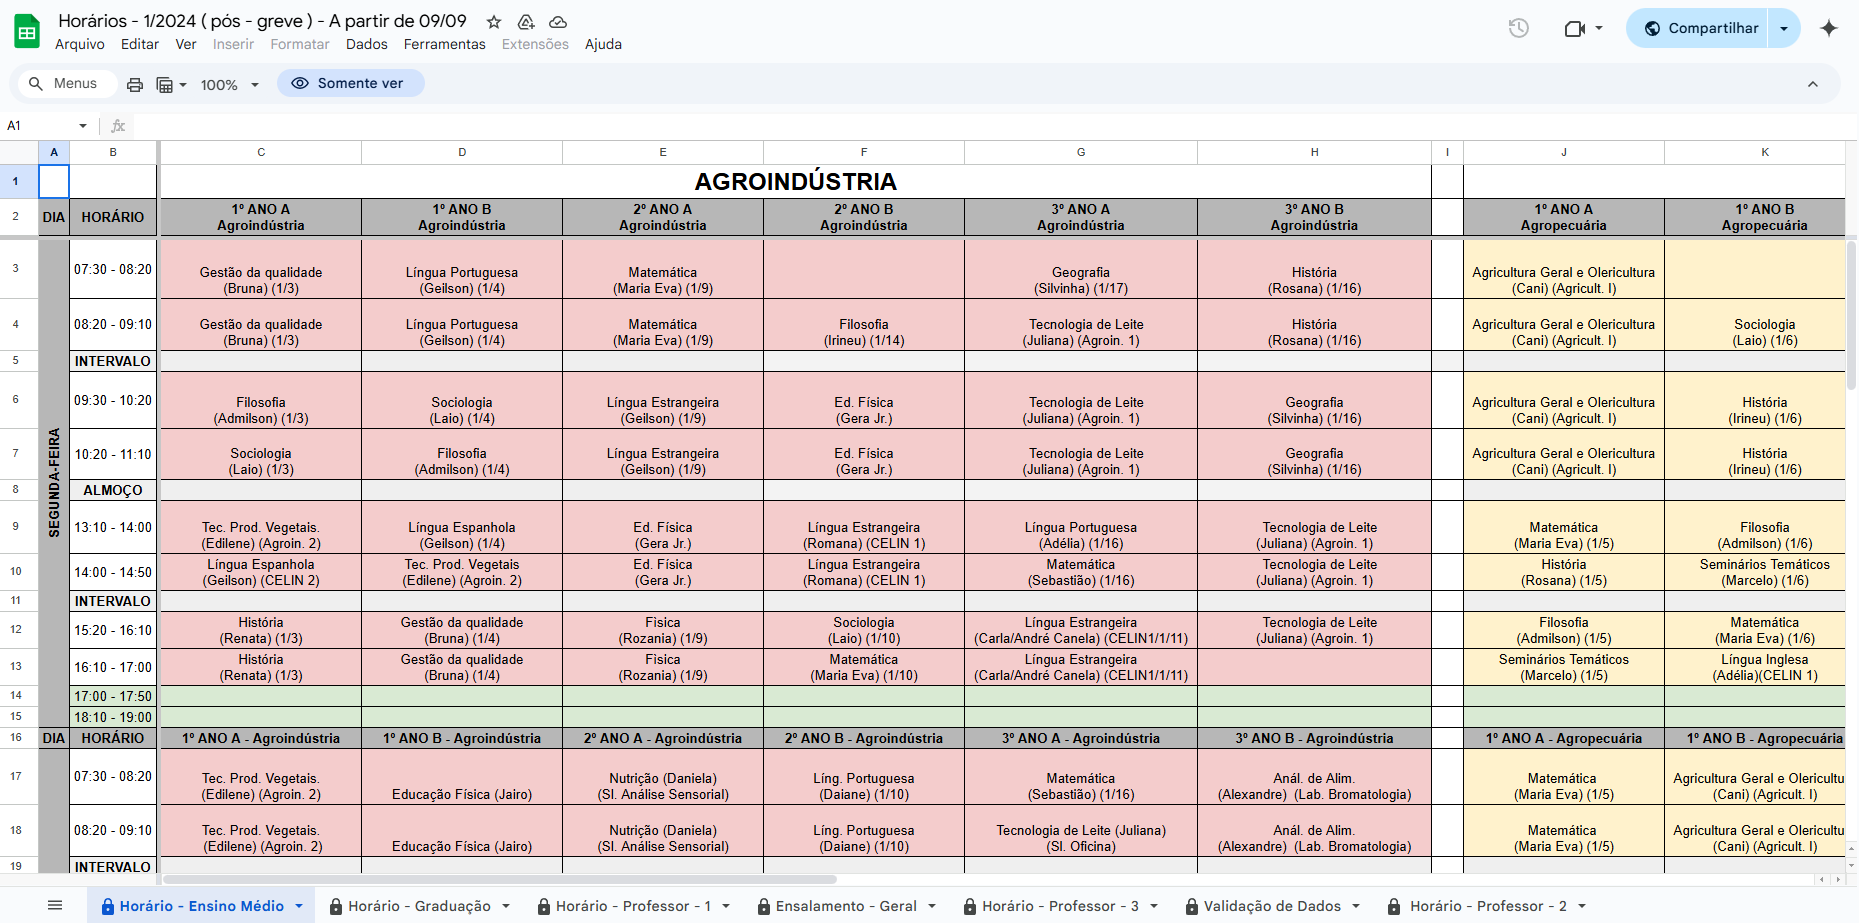
\includegraphics[width=0.9\textwidth]{Figuras/plan-ant-1.png}
                \caption*{Fonte: AUTOR (2024)}
                \label{fig_plan-ant_1}
            \end{figure}

            \begin{figure}[htb]
                \centering
                \caption{Horário - Graduação}
                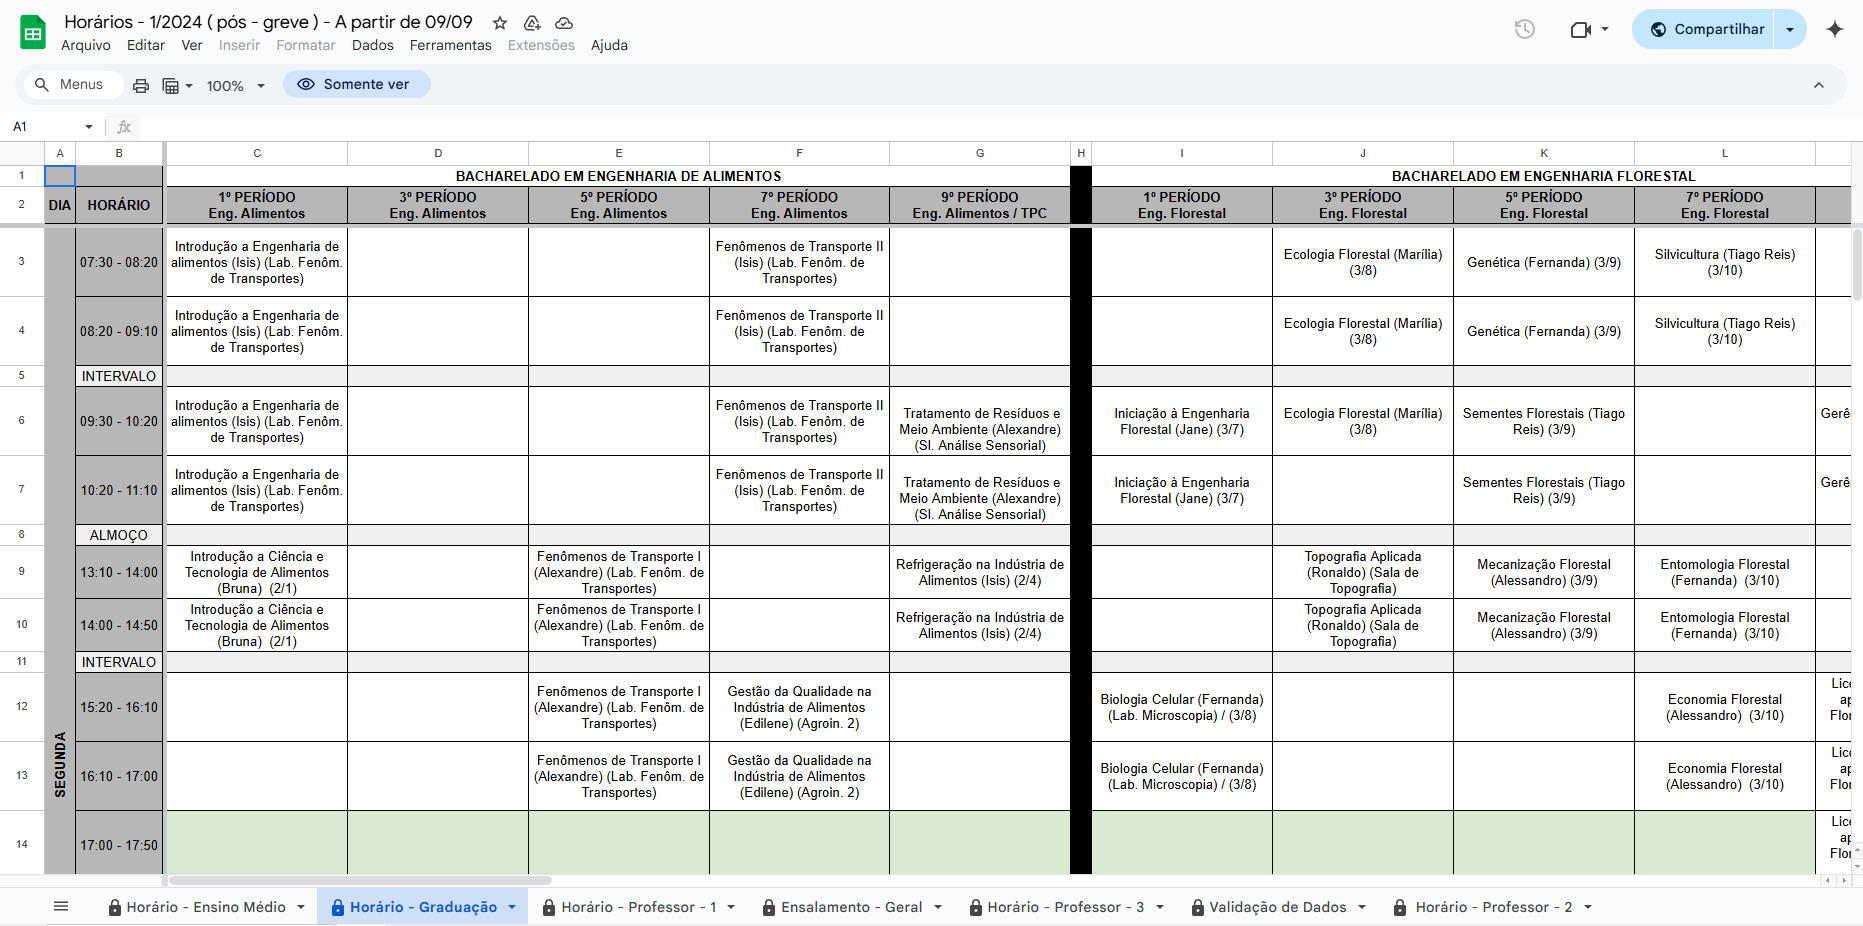
\includegraphics[width=0.9\textwidth]{Figuras/plan-ant-2.png}
                \caption*{Fonte: AUTOR (2024)}
                \label{fig_plan-ant_2}
            \end{figure}
            
            \item \textbf{Solução proposta}: Diante das limitações identificadas, a modernização do sistema de exibição de horários é fundamental para garantir maior eficiência e acessibilidade na consulta das informações.
            \item \textbf{Funcionalidades desejadas}: A plataforma deverá ter um menu com quatro opções que permita a consulta de horários dos cursos técnicos, dos cursos superiores, de um professor específico e de uma sala específica. O design deve seguir a identidade visual do IFNMG - Campus Salinas, adotando as cores institucionais para manter a padronização visual. Além disso, é essencial que a plataforma ofereça a opção de download dos horários e seja totalmente responsiva, garantindo uma navegação eficiente em dispositivos móveis, que muitas vezes são o principal meio de acesso utilizado pelos usuários.
        \end{enumerate}
    \end{itemize}
\end{itemize}

\section{Front-end}

\begin{itemize}
    \item \textbf{Protótipo do Front-end}: Outra atividade importante foi a prototipação, que se tratava da validação de um protótipo proposto ao setor de acordo com a solução desejada. A grande vantagem de utilizar o protótipo é que o setor teve uma visão prévia da solução final, e pôde rapidamente validar ou solicitar alguma mudança, permitindo modificações antes do desenvolvimento do sistema. Para isso, utilizou-se o \textit{Figma}, uma ferramenta que oferece recursos como armazenamento em nuvem e animações. Esses recursos permitiram um armazenamento seguro, além de possibilitar o compartilhamento, acompanhamento de atualizações e modificações em tempo real.
    
    \item \textbf{Desenvolvimento do Front-end}: Para o processo de desenvolvimento da interface, foi utilizado o \textit{Next.js}, que permite a construção de aplicações \textit{front-end} reativas que se adaptam dinamicamente a mudanças e eventos, mantendo uma experiência do usuário responsiva, eficiente e de alto desempenho que responde de forma eficiente a eventos em tempo real. Um dos principais fatores da escolha do \textit{Next.js} é sua integração perfeita com o \textit{Tailwind CSS}, que facilita a criação de interfaces modernas, responsivas e altamente customizáveis. Isso simplifica o processo de estilização, pois se puderam utilizar as classes pré-definidas para aplicar estilos consistentes em toda a aplicação.

    \item \textbf{Arquitetura do Front-end}: Foi aplicada a arquitetura do Next.js, baseada em componentes independentes e reutilizáveis, permitindo maior modularidade e promovendo um alto nível de desacoplamento, garantindo que mudanças pontuais não afetem os demais.
\end{itemize}

\section{Back-end}

\begin{itemize}
    \item \textbf{Google Sheets como Banco de Dados}: Para o processo de desenvolvimento do banco de dados da plataforma, foi utilizado o \textit{Google Sheets}, que oferece uma interface intuitiva para a criação e manipulação de planilhas. A flexibilidade da ferramenta permitiu que funcionasse como um banco de dados leve e eficiente. Com a capacidade de organizar dados em linhas e colunas, o \textit{Google Sheets} facilitou o armazenamento de dados estruturados, como registros de horários, nomes de cursos, turmas, professores e salas. Conforme \citeonline{ufsm2024}, sua estrutura pode ser associada à de um Sistema de Gerenciamento de Banco de Dados (SGBD) convencional, com as páginas da planilha representando as tabelas e suas colunas equivalentes às colunas de um SGBD, onde cada linha da planilha representa um registro específico da página.

    Para garantir que o sistema sempre exiba informações atualizadas, o setor de ensino ficou responsável por copiar os dados mais recentes de uma planilha privada e colá-los na planilha utilizada como banco de dados. Esse processo assegura que os usuários tenham acesso aos dados atualizados sem comprometer a segurança e integridade das informações, mantendo a flexibilidade operacional e permitindo que o setor preserve a forma habitual de realizar ajustes nos dados. Não é necessário criar uma nova planilha para o funcionamento da plataforma. No entanto, caso isso ocorra, é crucial que a nova planilha siga exatamente a mesma estrutura da original, respeitando os nomes das guias e os intervalos de células definidos para a extração dos dados. Alterações como renomear guias, excluir ou modificar a posição das células podem comprometer a funcionalidade da plataforma.
    
    \item \textbf{Google Sheets API}: A integração com \textit{Google Sheets} foi realizada por meio de sua API, que permitiu acessar os dados da planilha de forma automatizada. Essa operação possibilitou a extração das informações, tornando-as prontas para uso no sistema.
    \item \textbf{Implementação do Back-end:} Para o desenvolvimento do \textit{back-end} da aplicação, foi utilizado o \textit{Spring Boot}, que facilita a criação de sistemas web robustos e escaláveis. A escolha se justificou pela flexibilidade, facilidade de configuração e ampla adoção no mercado. Tornando-se essencial para estabelecer a conexão com a API do \textit{Google Sheets}, recebendo os dados e enviando-os ao \textit{front-end} de forma estruturada e confiável. Ademais, para garantir a segurança, foi configurada para permitir apenas operações de leitura, impedindo qualquer tentativa de modificação na planilha do sistema.
    \item \textbf{Arquitetura do Back-end}: Foi organizado segundo o padrão MVC, que separa a apresentação e a interação dos dados do sistema. Essa divisão entre Model, View e Controller garante que as alterações nos dados ocorram de modo independente de sua apresentação, permitindo diferentes formas de exibir os dados.
\end{itemize}

\subsection{Integração Front-end com Back-end}

A integração foi realizada por meio de uma \textit{API RESTful} desenvolvida com \textit{Spring Boot}, que atuou como intermediária entre a interface construída em \textit{Next.js} e os dados armazenados no \textit{Google Sheets}. O \textit{front-end} enviava requisições HTTP ao \textit{back-end} para acessar informações como horários de cursos, turmas, professores e salas. Essas solicitações eram processadas pelo \textit{back-end}, que recuperava os dados por meio da \textit{Google Sheets API} e os retornava no formato \textit{JSON}. Dessa forma, as informações foram exibidas na interface de maneira clara, organizada e dinâmica.

Alterações feitas diretamente no \textit{Google Sheets} apareceram automaticamente na plataforma, pois a API acessou os dados atualizados da planilha. Assim, eliminou-se a necessidade de atualizações manuais ou processos de sincronização, otimizando a experiência do usuário final. O \textit{back-end} foi implementado com mecanismos de controle de acesso, garantindo a segurança e preservando a integridade das informações. A integração promovida conectou as diferentes partes do sistema de maneira eficiente, promovendo uma experiência confiável e responsiva.

\subsection{Testes}

A verificação da plataforma foi realizada ao longo dos meses de setembro e outubro de 2024, período em que o desenvolvedor conduziu testes técnicos e o setor de ensino, na função de cliente, validou a aplicação em ambiente real de uso. Após os ajustes finais, a plataforma foi oficialmente disponibilizada em novembro de 2024. Durante o desenvolvimento, os testes foram organizados da seguinte forma:

\begin{itemize}
    \item \textbf{Teste Unitário}: Focado no back-end, com ênfase na leitura dos dados da planilha em diferentes cenários e na verificação do comportamento das requisições.
    \item \textbf{Teste de Componentes}: Realizado no front-end, avaliando a exibição correta dos dados, o funcionamento das rotas, os estados dos componentes, os estilos aplicados e a responsividade em dispositivos móveis.
    \item \textbf{Teste de Sistema}: Executado localmente, simulando o comportamento da aplicação em um ambiente de produção. Para isso, foram realizados os builds do back-end e do front-end, permitindo testar o funcionamento completo da plataforma. Os testes incluíram a configuração das variáveis de ambiente, testando a leitura dos dados da planilha, a correta exibição das informações no navegador e a comunicação por meio de requisições. O objetivo foi verificar se a integração entre os módulos e as interações entre os componentes do sistema ocorriam de forma correta.
\end{itemize}

Esse processo colaborativo foi essencial para identificar falhas, validar funcionalidades e ajustar a aplicação conforme as necessidades apresentadas.

\subsection{Deploy}

Para disponibilizar o sistema na internet, o \textit{front-end} foi implementado em uma conta particular na \textit{Vercel}\footnote{https://vercel.com/docs}, uma plataforma especializada no deploy de aplicações web baseadas em \textit{JavaScript}, como o \textit{Next.js}, que oferece uma integração direta e otimizada para esse tipo de aplicação. O \textit{back-end}, por sua vez, foi hospedado em uma conta privada na \textit{Koyeb}\footnote{https://www.koyeb.com/docs}, uma plataforma serverless amigável para desenvolvedores, projetada para permitir que empresas implantem aplicativos confiáveis e escaláveis globalmente.

\subsection{Armazenamento do Código e Integração}

Para a hospedagem do código, foi utilizado o GitHub\footnote{https://github.com/}, um repositório de hospedagem de serviços Git. Podendo ser considerado como uma rede social para desenvolvedores, além de uma plataforma colaborativa. Ao utilizá-lo, os programadores podem interagir e colaborar em repositórios de código aberto, permitindo que realizem downloads, cooperem, compartilhem, além de outras funcionalidades \cite{silva2024biblioteca}.

Uma conta do GitHub foi vinculada às plataformas Vercel e Koyeb para permitir o acesso direto aos arquivos do projeto, viabilizando a integração necessária para o deploy. Na Koyeb, o Docker foi utilizado para criar e gerenciar contêineres, garantindo o isolamento e a portabilidade do \textit{back-end}, desenvolvido com \textit{Spring Boot}. Dessa forma, proporcionou o funcionamento adequado de ambas as partes do sistema.

\section{Ambiente de desenvolvimento}

Para a codificação do sistema, foi utilizado o Visual Studio Code\footnote{https://code.visualstudio.com}, um editor de código-fonte criado pela Microsoft com o objetivo de auxiliar programadores na criação de softwares. Sendo amplamente adotado para escrever, editar e gerenciar os códigos durante o desenvolvimento de um projeto \cite{silva2024biblioteca}.

A escolha desse editor se justificou por sua facilidade na construção de códigos e por sua interface limpa, personalizável e organizada.

\section{Avaliação da Plataforma}

Para avaliar a eficácia da plataforma, foi realizada uma análise baseada na percepção do responsável pela gestão acadêmica que participou do levantamento de requisitos. A reunião foi agendada com o Coordenador de Ensino Superior/Diretor de Ensino Substituto do Campus Salinas, no seu caso, o professor Frederico Ventura Batista, para fornecer feedbacks detalhados sobre o sistema desenvolvido.

A condução da entrevista para a avaliação da plataforma foi realizada conforme os seguintes passos:
\begin{itemize}
    \item \textbf{Preparação}:
    \begin{itemize}
        \item \textbf{Agendamento}: A reunião foi marcada com antecedência, com a confirmação da disponibilidade do Sr. Frederico Ventura Batista.
        \item \textbf{Objetivos}: Foram claramente definidos para verificar se a plataforma atende às necessidades do setor e identificar possíveis pontos de melhoria.
    \end{itemize}
    \item \textbf{Entrevista}: A entrevista foi iniciada com uma explicação ao entrevistado sobre o objetivo do questionário e o propósito da avaliação. Em seguida, o entrevistado respondeu às perguntas apresentadas.
    \item \textbf{Perguntas}: A entrevista foi guiada por um questionário com seis perguntas abertas, cujas questões e respostas estão registradas no Apêndice \ref{apendiceB}. Isso permitiu coletar informações sobre a experiência de uso e as percepções do setor em relação à solução desenvolvida.
    \item \textbf{Documentação}:
    \begin{itemize}
        \item \textbf{Registro Detalhado}: Durante a entrevista, foram registrados os principais pontos discutidos, entre eles:
        \begin{enumerate}
            \item \textbf{Usabilidade e navegação}: A plataforma é mais fácil de usar em comparação com a planilha anteriormente utilizada.
            \item \textbf{Eficiência na exibição dos horários}: As informações são apresentadas de forma clara e organizada, facilitando a consulta.
            \item \textbf{Redução de dificuldades operacionais}: O sistema ajudou a minimizar as dificuldades no gerenciamento dos horários acadêmicos e melhorou o fluxo de trabalho.
            \item \textbf{Satisfação geral}: A plataforma atendeu às expectativas do setor e se mostrou uma solução eficaz para a gestão dos horários acadêmicos.
            \item \textbf{Melhorias e atualizações}: A integração de outras ferramentas de apoio à gestão do ensino, como a criação de uma nova funcionalidade para validação dos dados da planilha e adição de links diretos para os sistemas complementares, como o de reserva de horários, o que exibe os locais do instituto e o de gerenciamento de reserva de salas.
            \item \textbf{Garantia de Disponibilidade}: O software será transferido para a instituição, com a elaboração de uma documentação para orientar a manutenção do sistema. (essa parte ainda não fiz)
        \end{enumerate}
    \end{itemize}
\end{itemize}

A avaliação foi conduzida de maneira ética e transparente, garantindo que os resultados obtidos refletissem de forma precisa a usabilidade e a efetividade da plataforma como substituta da planilha na exibição dos horários acadêmicos.

\section{Implementação de Melhorias e Atualizações}

Com base nas sugestões e críticas obtidas na avaliação da plataforma, foram realizadas melhorias voltadas a aprimorar a usabilidade e expandir as funcionalidades do sistema. O histórico das versões desenvolvidas até o momento:

\begin{itemize}
    \item \textbf{v.1.0.0}: A primeira versão correspondeu à versão inicial do projeto, que disponibilizou quatro opções no menu principal para a consulta dos horários acadêmicos. Essas opções permitiam visualizar os horários dos cursos técnicos, dos cursos superiores, de um professor específico e de uma sala específica.
    \item \textbf{v.2.0.0}: Na segunda versão, foram implementadas melhorias e atualizações a partir da avaliação realizada. As principais mudanças foram:
    \begin{itemize}
        \item Desenvolvimento de uma nova tela de login para entrar na tela de validação de dados.
        \item Criação de uma nova planilha no Google Sheets com as credenciais de login para acessar a tela de validação de dados.
        \item Implementação de uma nova tela para a validação dos dados da planilha dos horários.
        \item Adição de um botão no menu principal da plataforma para direcionar para validação de dados.
        \item Inclusão de três novos botões no menu principal da plataforma com links externos para os sistemas complementares, como o de reserva de horários, o de visualização dos locais do instituto e o de gerenciamento de reserva de salas.
    \end{itemize}
\end{itemize}

Essas melhorias foram aplicadas considerando a viabilidade técnica e a relevância para os usuários, garantindo que a plataforma continue evoluindo para atender melhor às demandas do setor de ensino.

\section{Documentação}

Para garantir a correta manutenção e funcionamento da plataforma, foi elaborada uma documentação técnica da planilha com diretrizes essenciais sobre elementos estruturais que não podem ser alterados e regras que devem ser seguidas. Essa documentação abordou os seguintes aspectos:

\begin{itemize}
    \item \textbf{Estrutura e organização dos dados}: Foram descritos os procedimentos que devem ser realizados no início de cada semestre, como a atualização do ID da planilha com os horários acadêmicos na sua variável de ambiente, o uso de cópias da planilha original privada do setor de ensino para evitar alterações indesejadas, e os cuidados com a plataforma de deploy do back-end.
    \item \textbf{Regras para adição e atualização de informações}: A documentação apresentou exemplos de preenchimento dos campos na planilha, com orientações sobre a escrita padronizada. Os nomes das disciplinas não devem conter parênteses, os nomes dos professores precisam estar entre parênteses, e os nomes das salas igualmente devem estar entre parênteses, sem espaços extras. Algumas exceções são aceitas, como entradas com múltiplos professores ou informações adicionais. Na guia de Validação de Dados, deve-se evitar nomes com espaços ou parênteses antes e depois.
    \item \textbf{Padrões para nomes de guias e intervalos de células}: A documentação apresentou uma explicação sobre a estrutura de colunas e linhas do Google Sheets. Em seguida, foram definidos os nomes e intervalos das três guias essenciais para o correto funcionamento da plataforma, sendo elas:
    \begin{itemize}
        \item Horário - Ensino Médio, com intervalo B2:V76;
        \item Horário - Graduação, com intervalo B2:AW106;
        \item Validação de Dados, com intervalo A2:A.
    \end{itemize}
    É importante ressaltar que não devem ser feitas alterações nesses nomes ou na posição das células. Mudanças estruturais só devem ocorrer se forem realmente necessárias e com a devida atualização no código.
\end{itemize}

A documentação servirá como referência para futuros administradores da plataforma, assegurando a continuidade do sistema e facilitando sua manutenção.
\chapter{Resultados} 
\label{cap5_resultados}

\section{Front-end}

\subsection{Protótipos}

Após a reunião de levantamento de requisitos, protótipos das telas principais da plataforma foram construídos no Figma para validação junto ao setor. Esses protótipos estão disponíveis no repositório do projeto, no endereço \url{https://github.com/Tomaz5556/Horarios-IFNMG-Salinas/blob/main/prototipos/figma.pdf}. A seguir, são apresentadas as telas desenvolvidas:

\begin{figure}[htb]
    \centering
    \caption{Protótipo da tela inicial}
    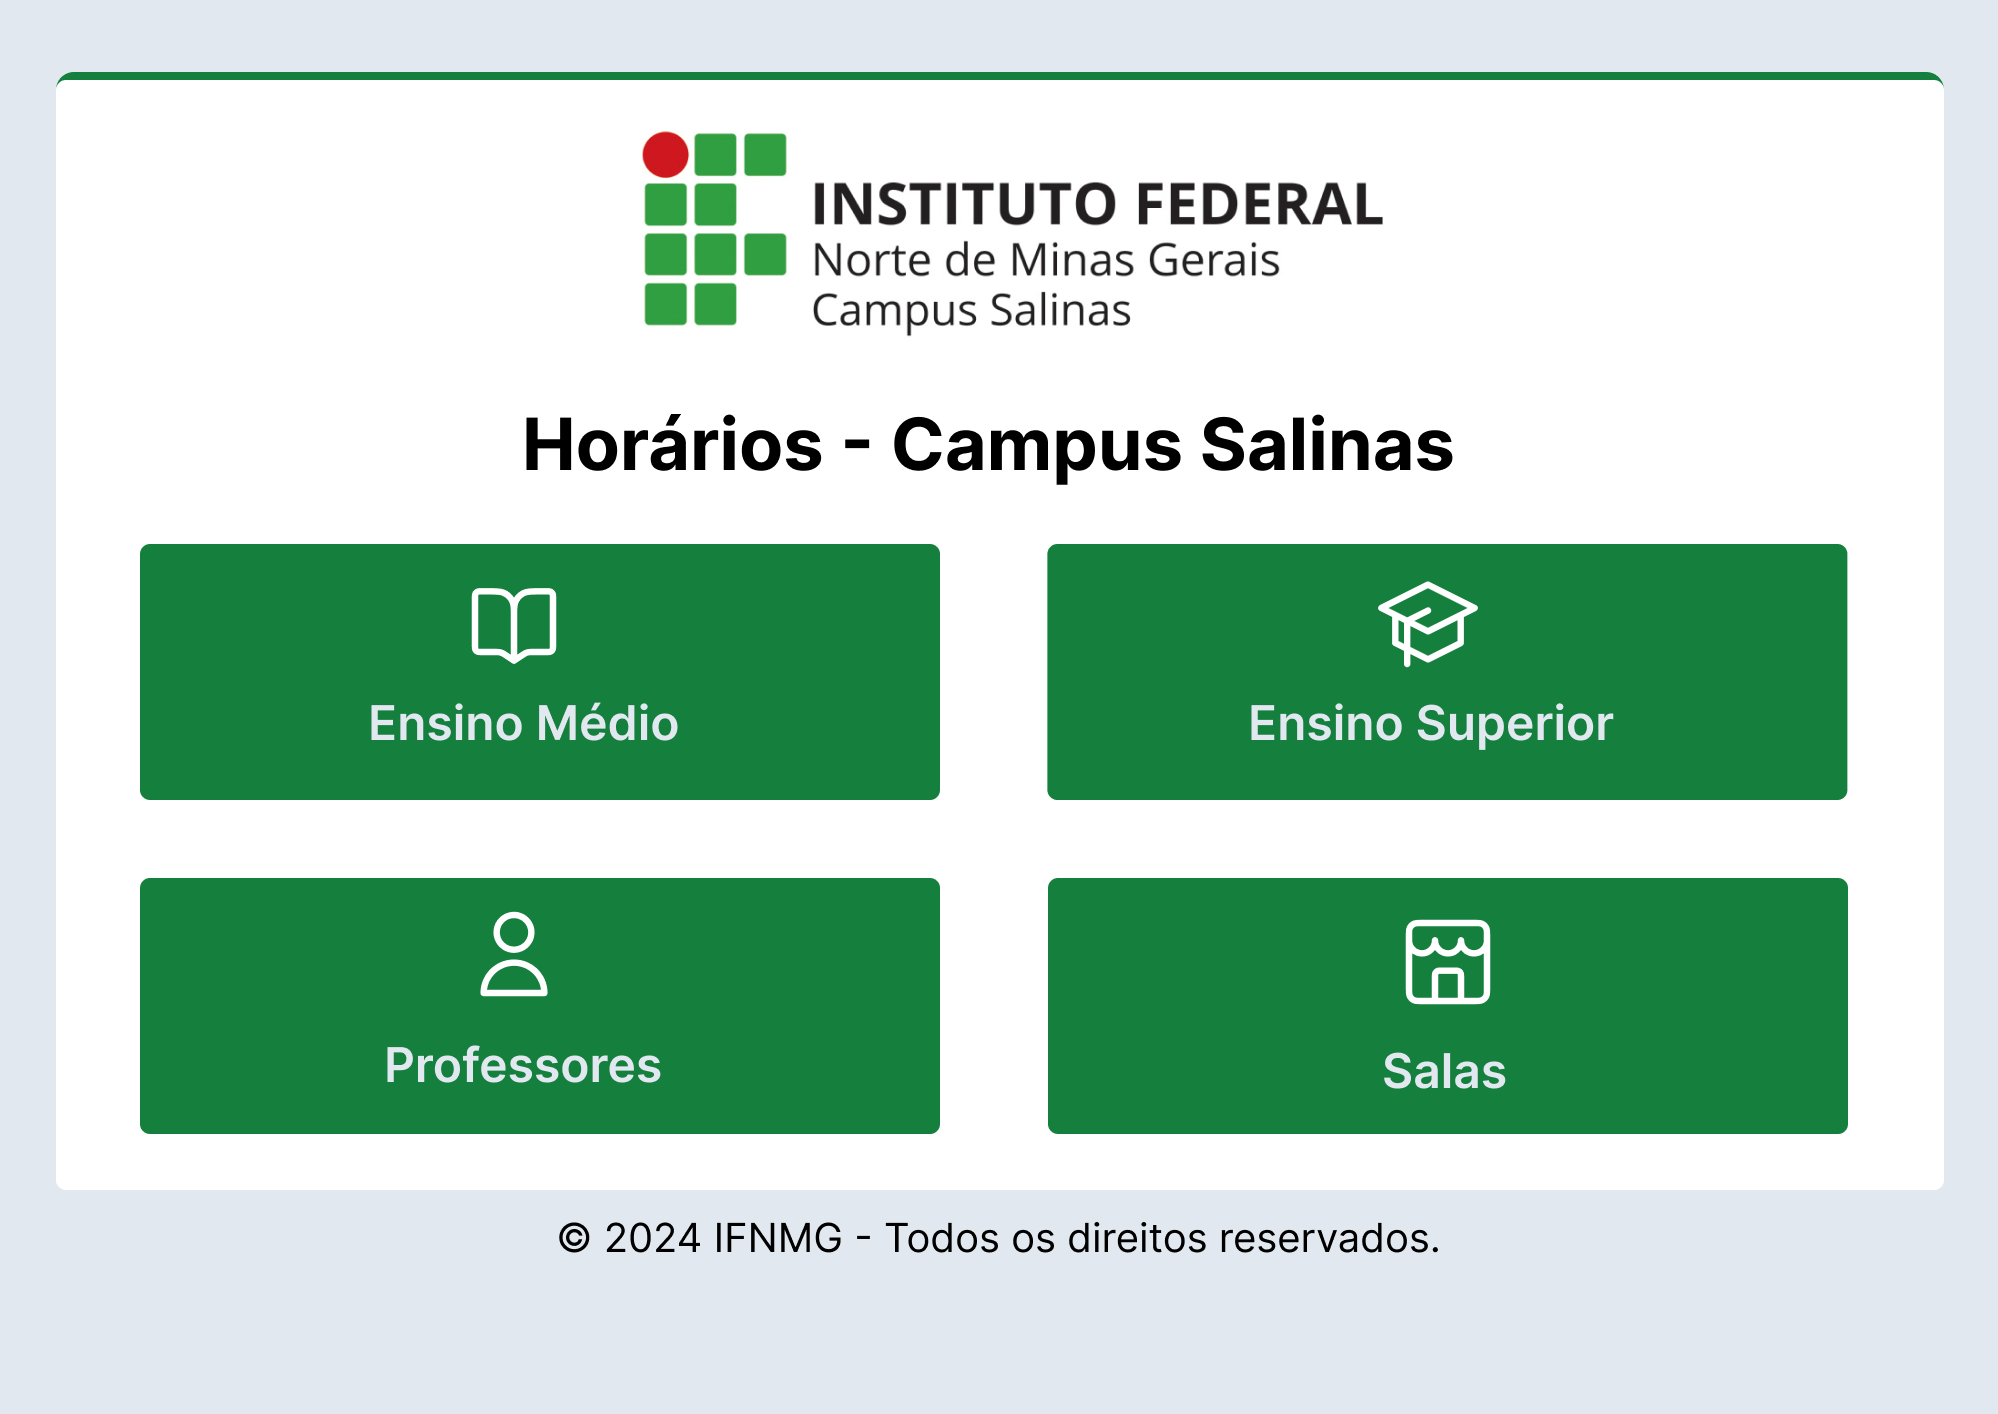
\includegraphics[width=1\textwidth]{Figuras/proto-1.png}
    \caption*{Fonte: AUTOR (2024)}
    \label{fig_proto_1}
\end{figure}

A Figura \ref{fig_proto_1} exibe o protótipo da tela inicial da plataforma, onde o usuário encontra quatro opções para selecionar o tipo de horário.

\begin{figure}[H]
    \centering
    \caption{Protótipo da tela dos cursos}
    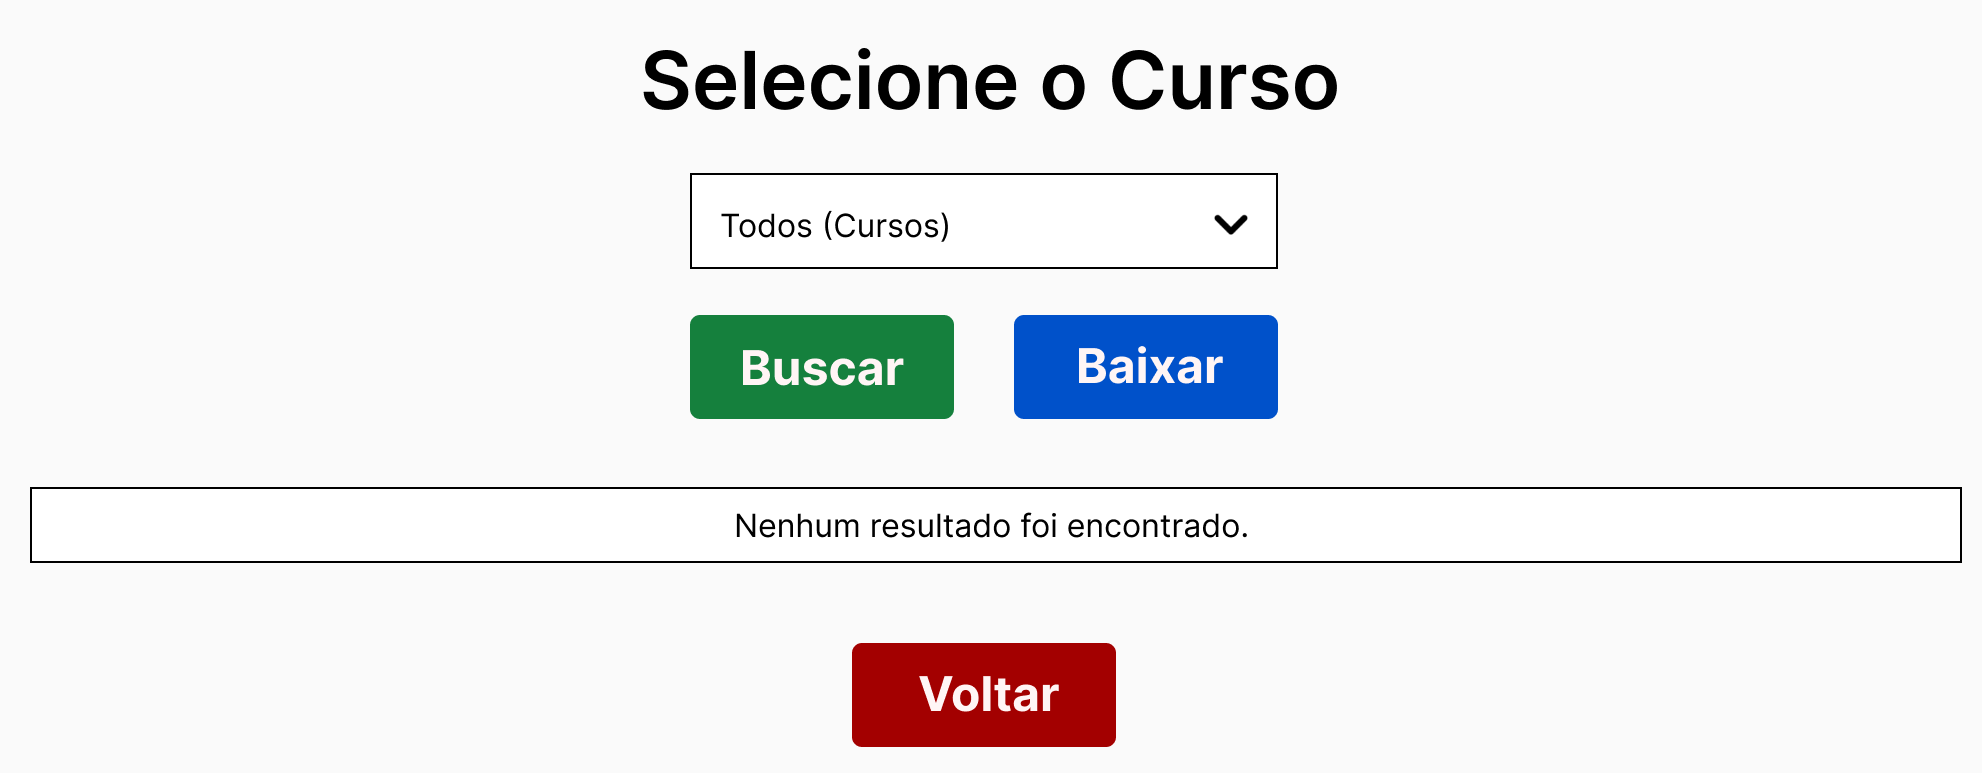
\includegraphics[width=1\textwidth]{Figuras/proto-2.PNG}
    \caption*{Fonte: AUTOR (2024)}
    \label{fig_proto_2}
\end{figure}

\begin{figure}[htb]
    \centering
    \caption{Protótipo da tela dos cursos preenchida}
    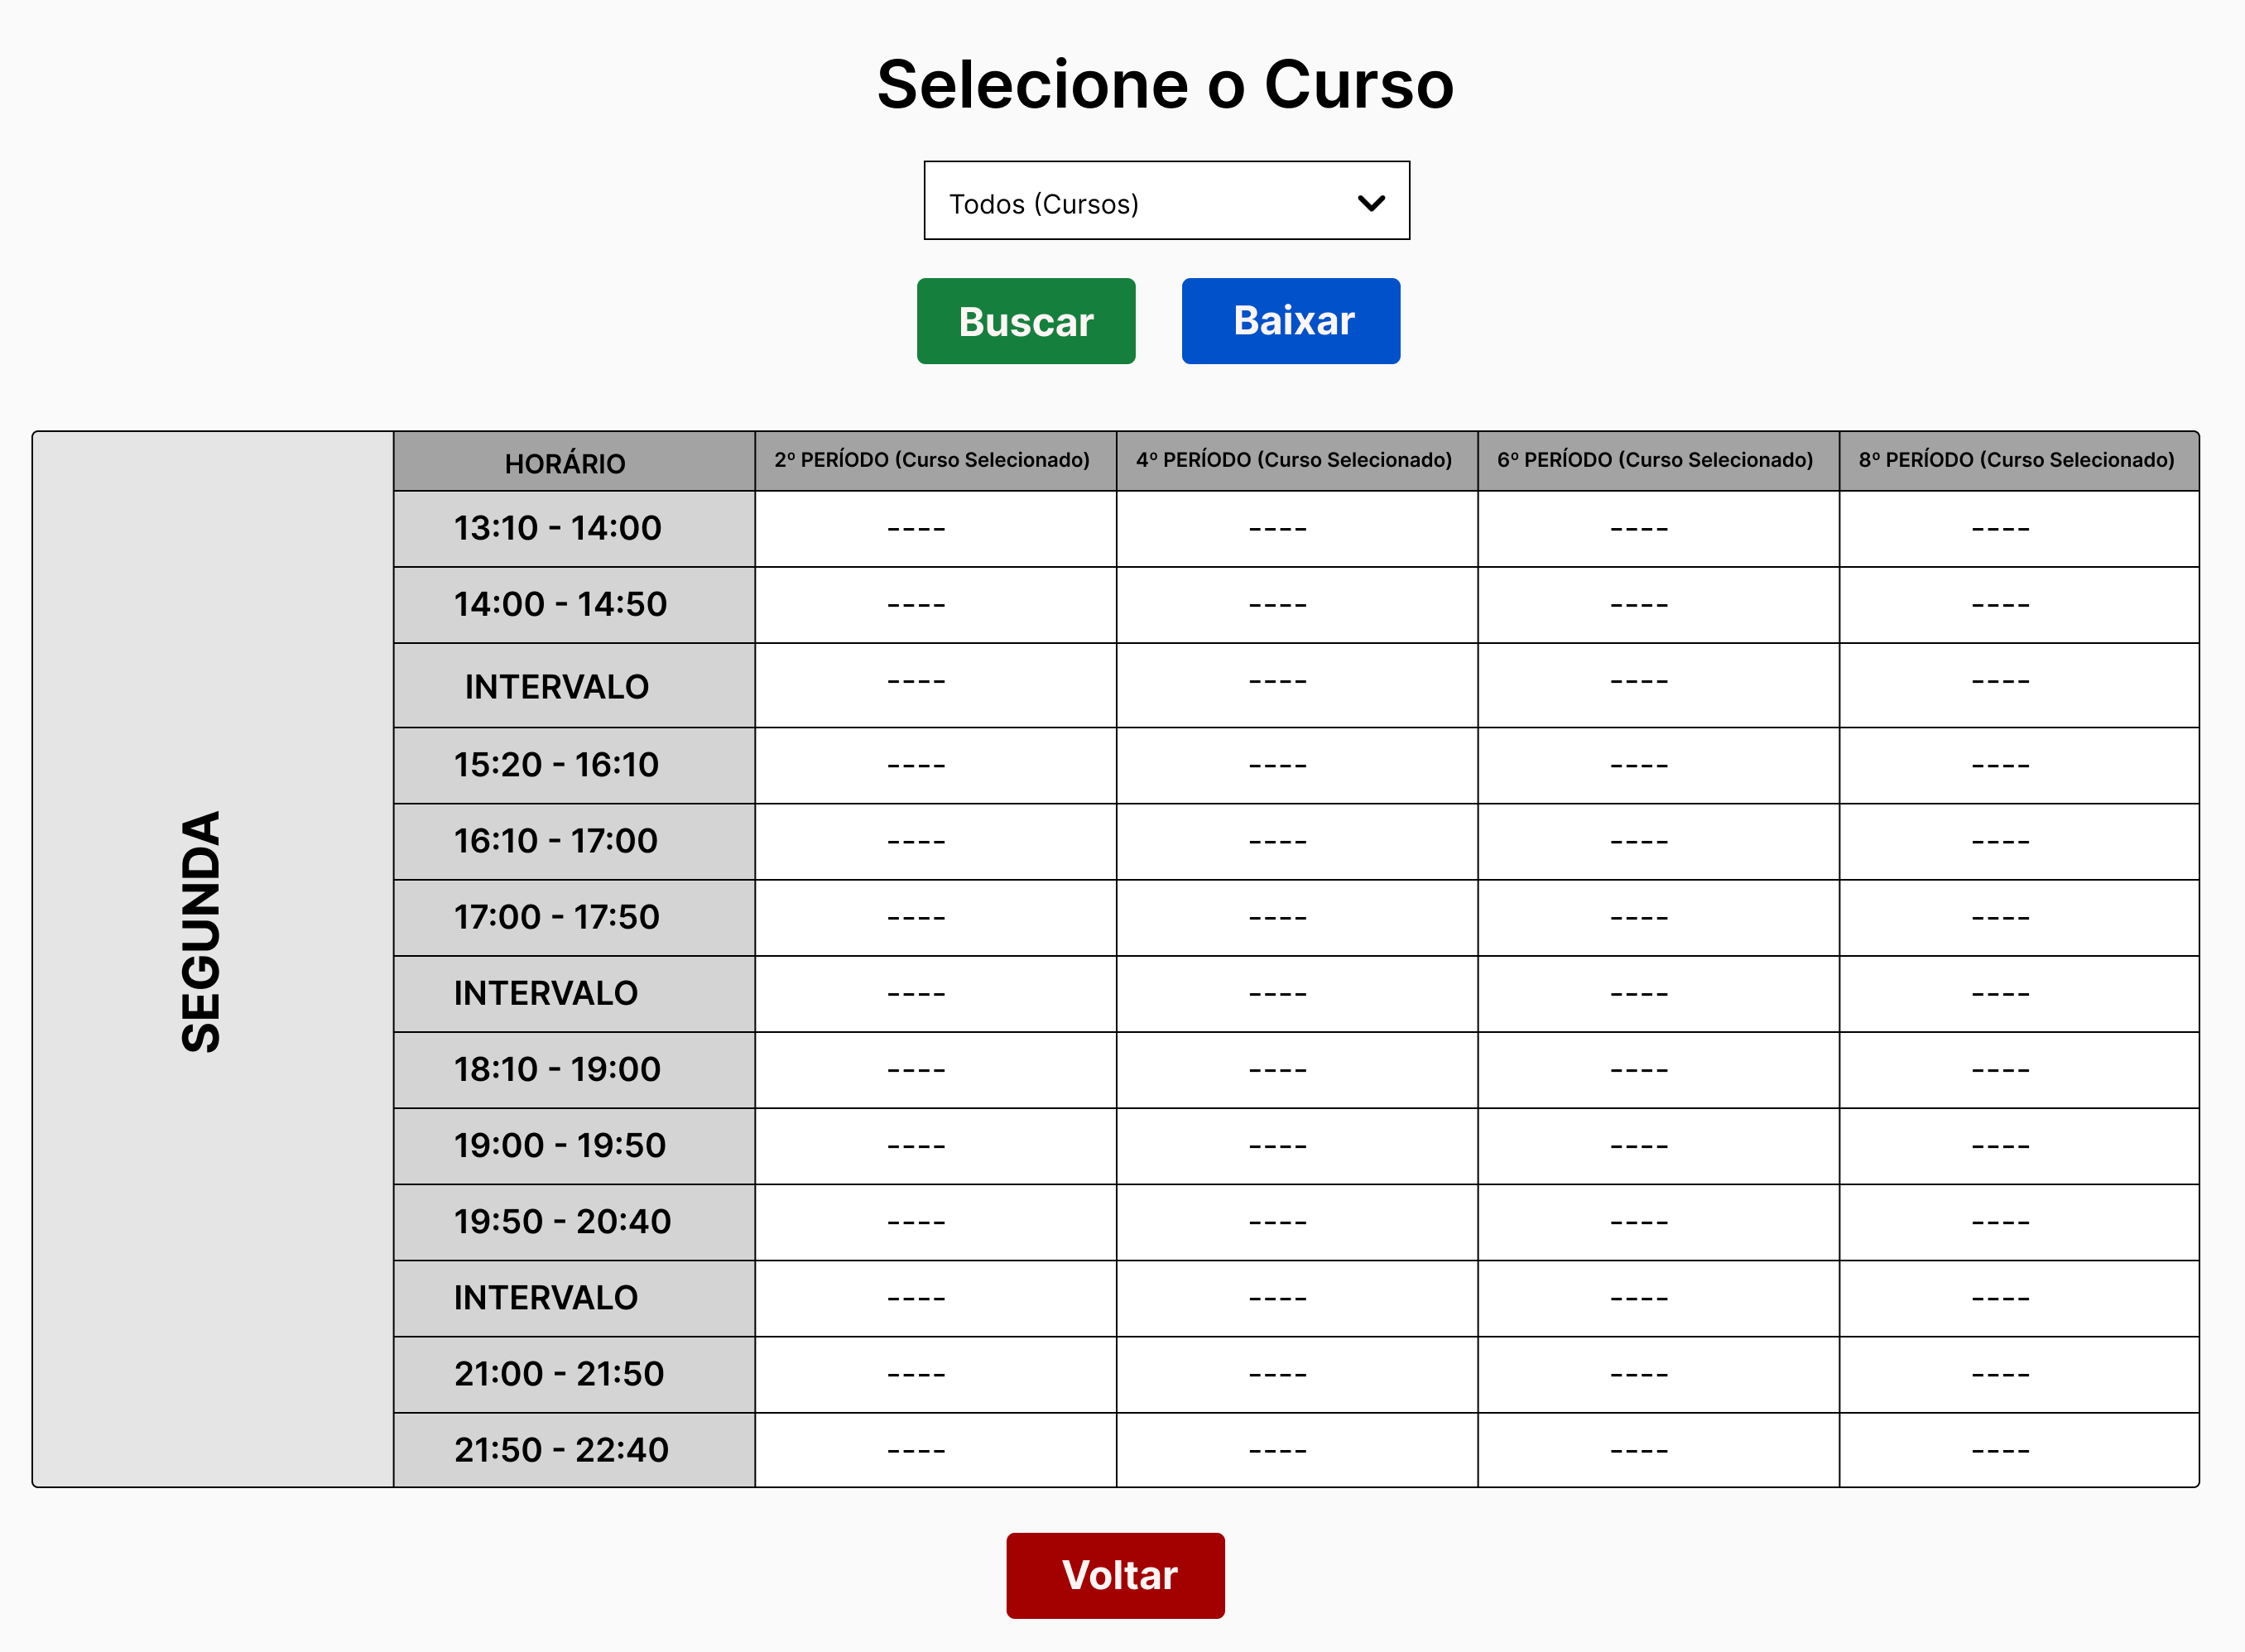
\includegraphics[width=1\textwidth]{Figuras/proto-3.PNG}
    \caption*{Fonte: AUTOR (2024)}
    \label{fig_proto_3}
\end{figure}

As Figuras \ref{fig_proto_2} e \ref{fig_proto_3} apresentam o protótipo da tela dos cursos, exibindo os horários e a distribuição das aulas ao longo da semana para um curso selecionado.

\begin{figure}[htb]
    \centering
    \caption{Protótipo da tela dos professores}
    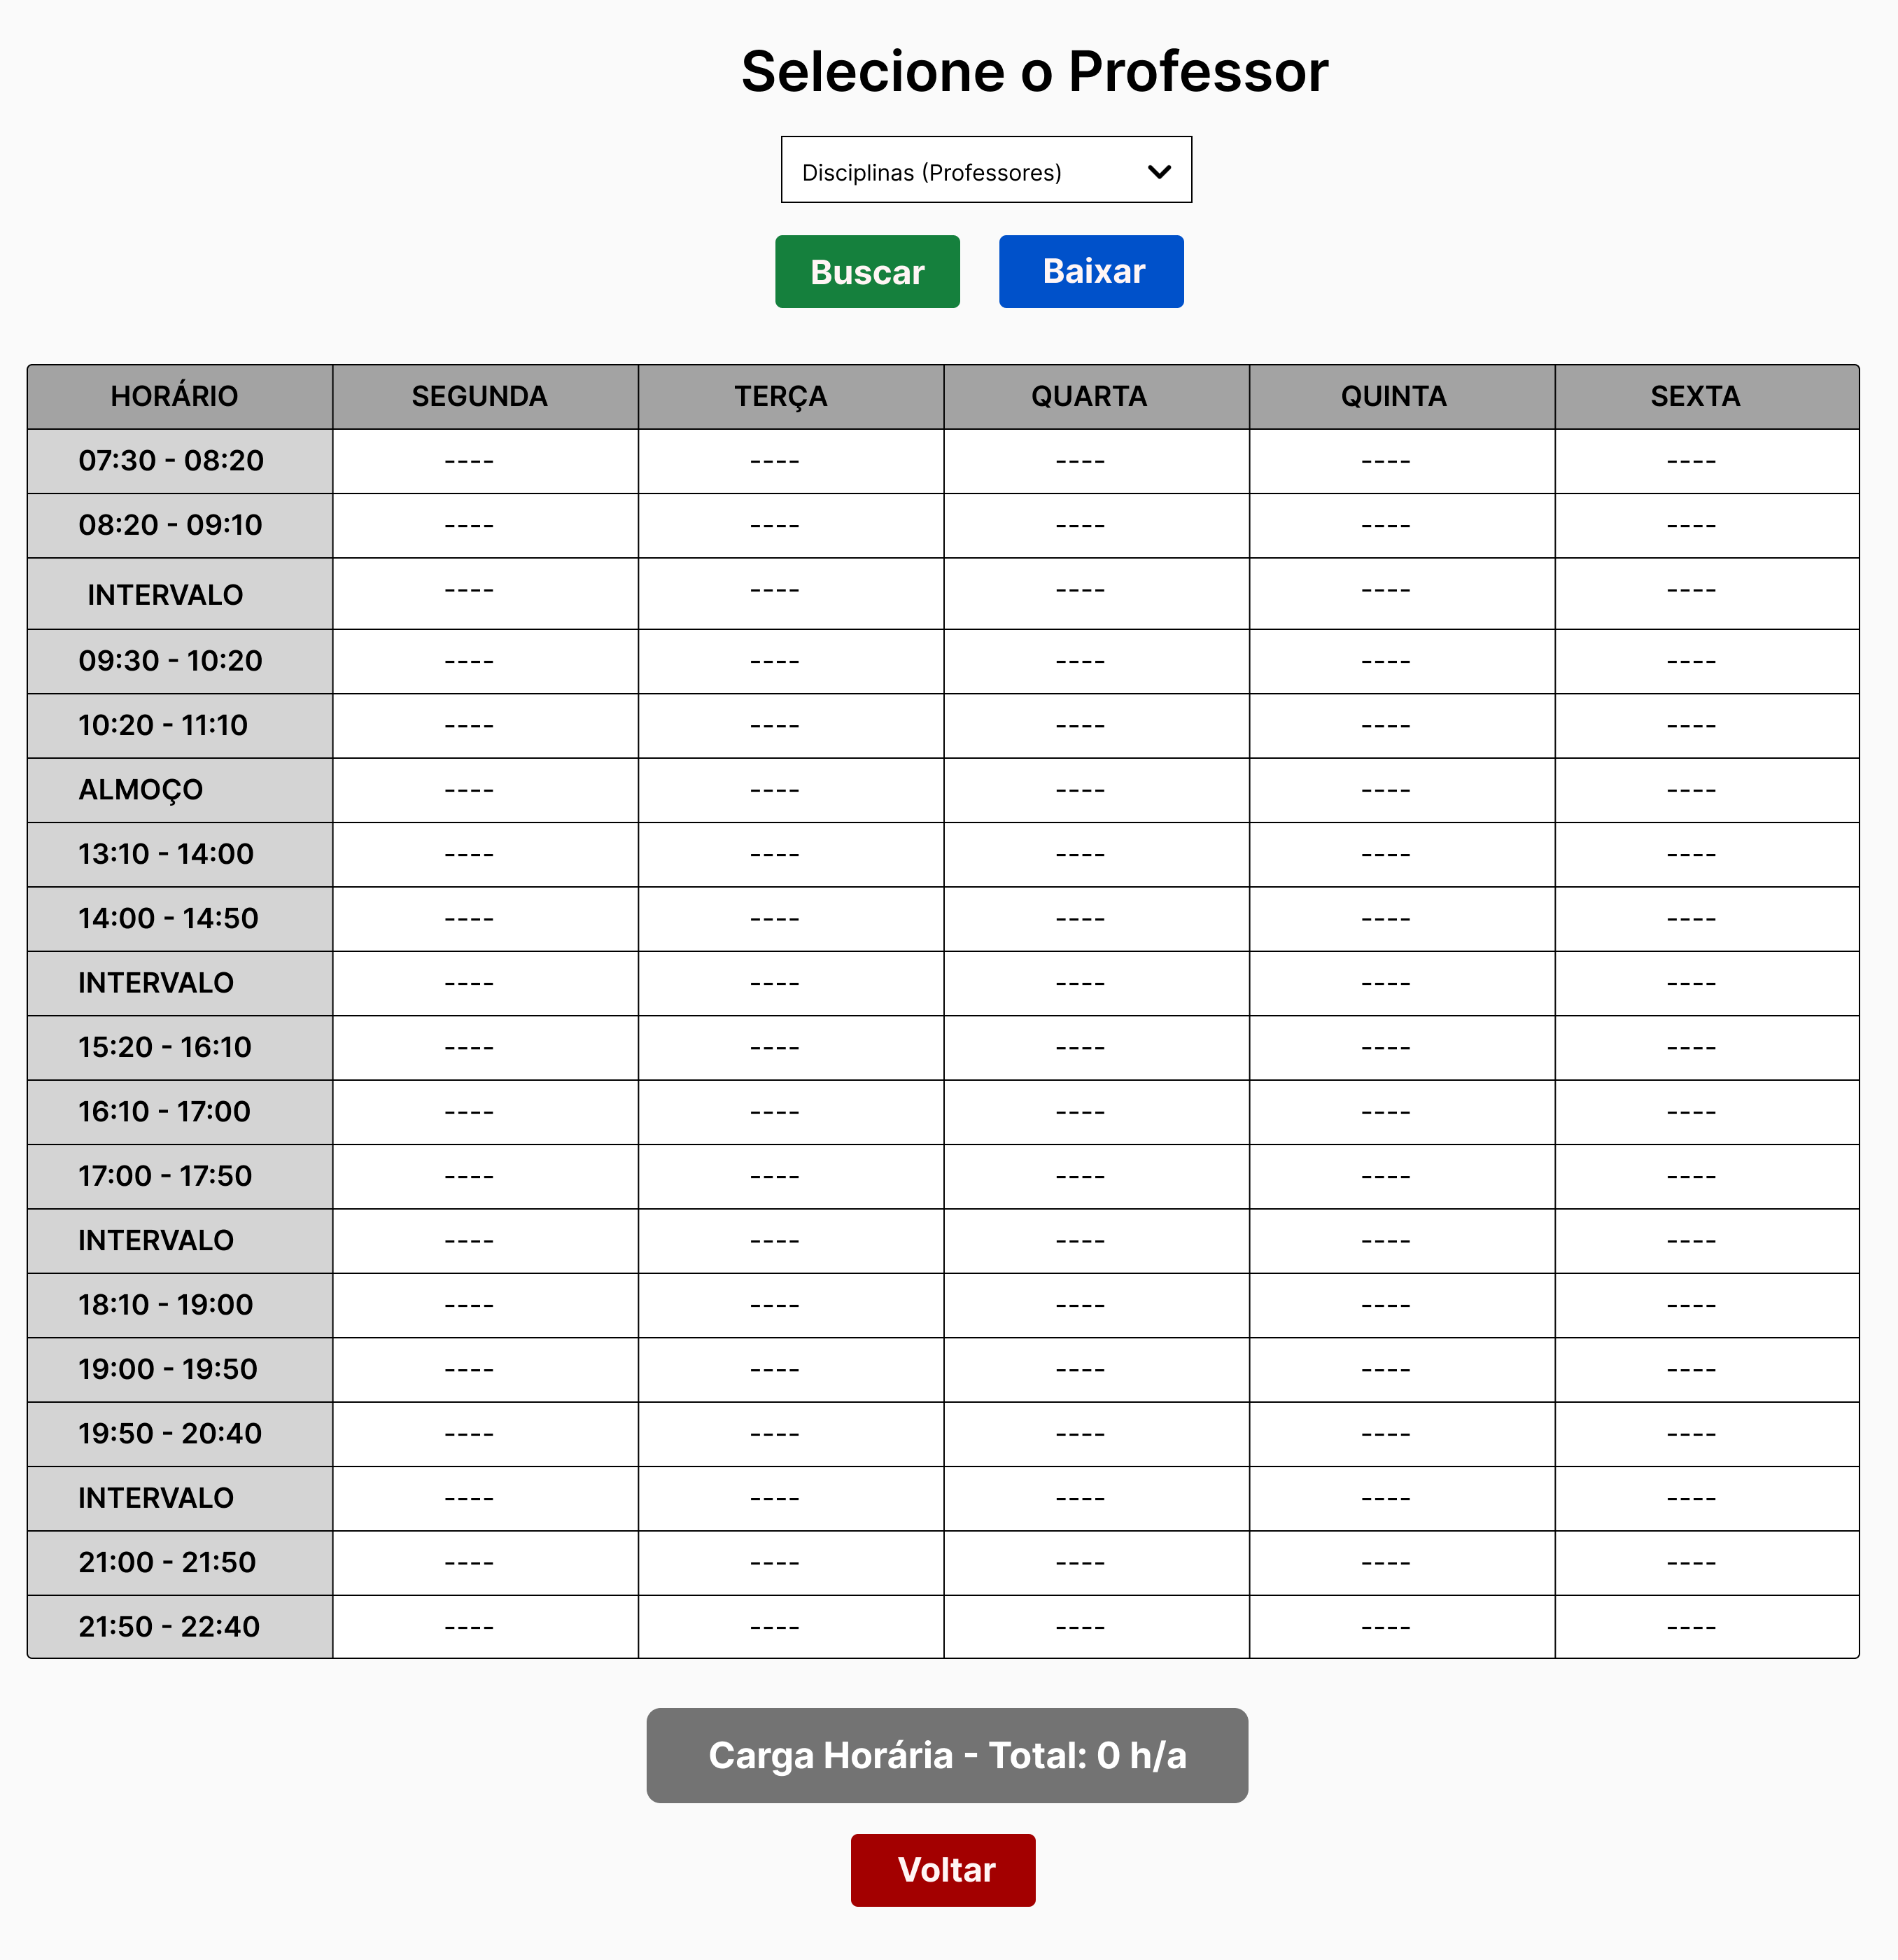
\includegraphics[width=1\textwidth]{Figuras/proto-4.PNG}
    \caption*{Fonte: AUTOR (2024)}
    \label{fig_proto_4}
\end{figure}

A Figura \ref{fig_proto_4} mostra o protótipo da tela dos professores, detalhando os horários das aulas e os dias da semana de um professor escolhido.

\begin{figure}[H]
    \centering
    \caption{Protótipo da tela das salas}
    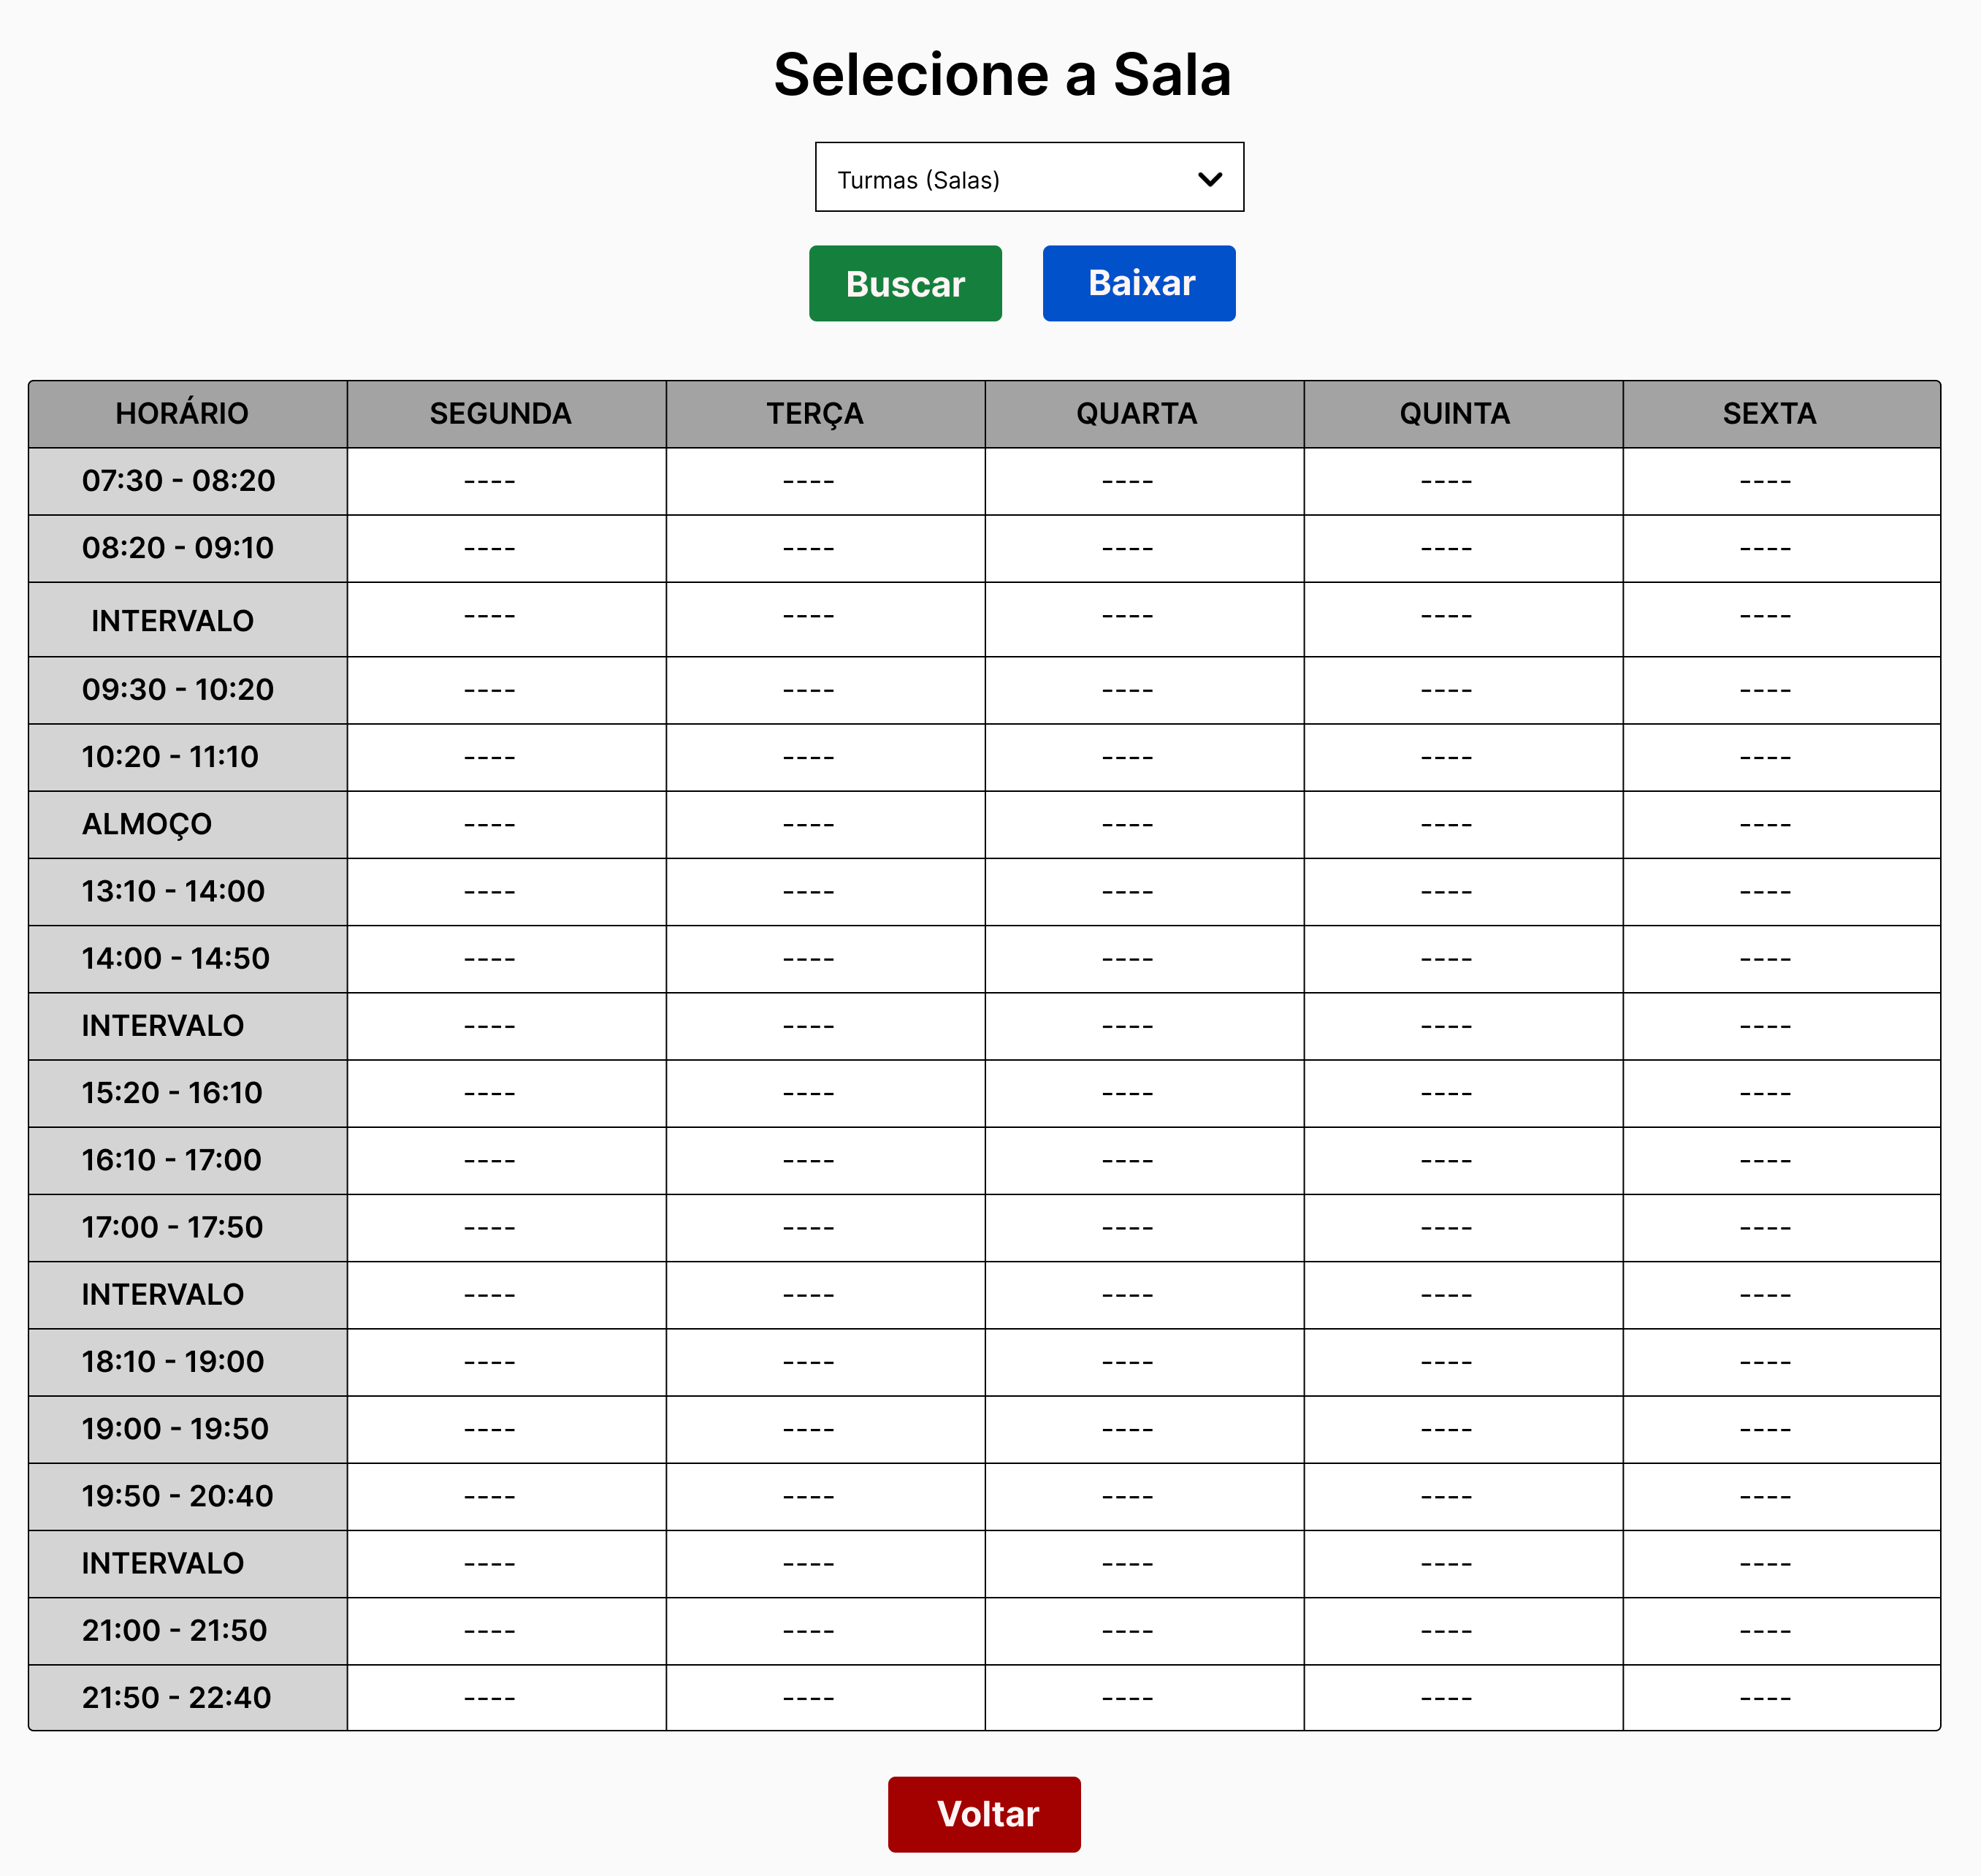
\includegraphics[width=1\textwidth]{Figuras/proto-5.PNG}
    \caption*{Fonte: AUTOR (2024)}
    \label{fig_proto_5}
\end{figure}

A Figura \ref{fig_proto_5} apresenta o protótipo da tela das salas, exibindo os horários de ocupação e os dias em que uma sala está reservada.

\subsection{Desenvolvimento do Front-end}

O front-end foi desenvolvido com o Next.js. Essa tecnologia possibilitou criar uma interface moderna e eficiente, capaz de responder dinamicamente a eventos e mudanças de estado, garantindo uma experiência de usuário fluida e responsiva. Todo o trabalho priorizou clareza na organização dos componentes, reutilização de elementos e facilidade de futuras evoluções, atendendo às necessidades do projeto com agilidade. O código está disponível no repositório do projeto em \url{https://github.com/Tomaz5556/Horarios-IFNMG-Salinas/tree/main/frontend}. A seguir, são exibidas as telas resultantes desse processo:

\begin{figure}[htb]
    \centering
    \caption{Menu principal com opções de botões de horários e outros serviços}
    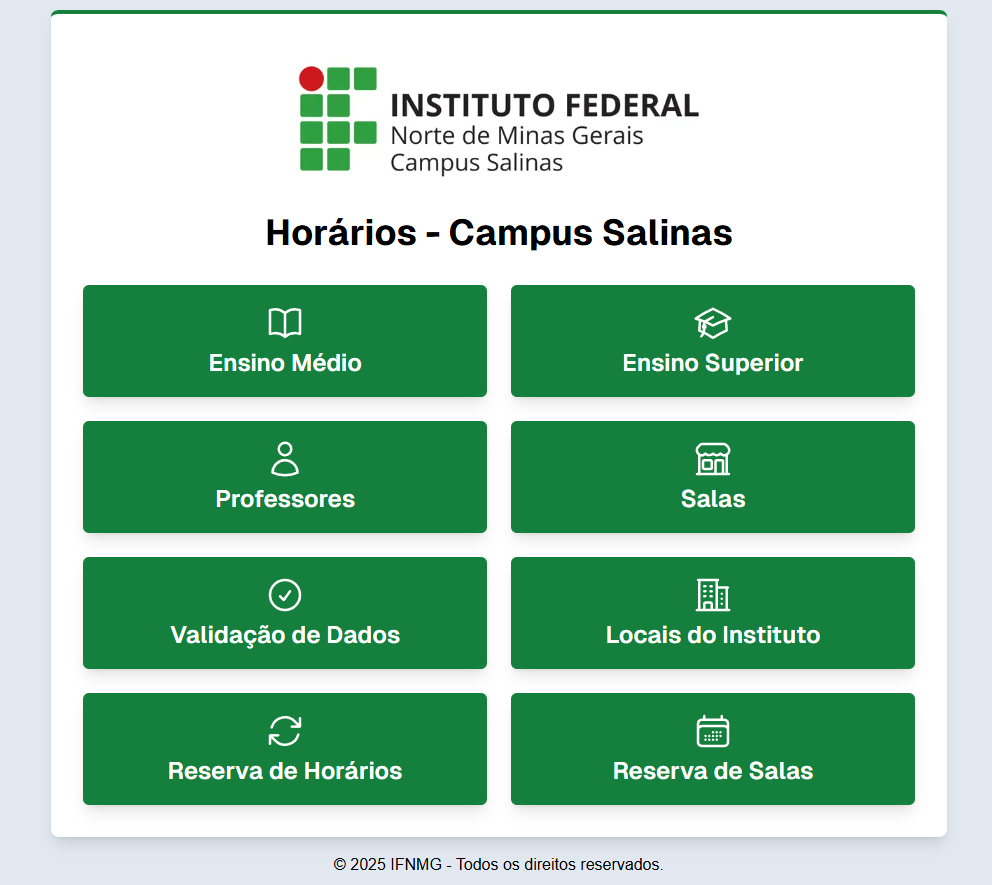
\includegraphics[width=1\textwidth]{Figuras/front-1.png}
    \caption*{Fonte: AUTOR (2025)}
    \label{fig_front_1}
\end{figure}

A Figura \ref{fig_front_1} mostra o menu principal da plataforma, com botões para consulta de horários e acesso a outros serviços.

\begin{figure}[htb]
    \centering
    \caption{Tela dos cursos}
    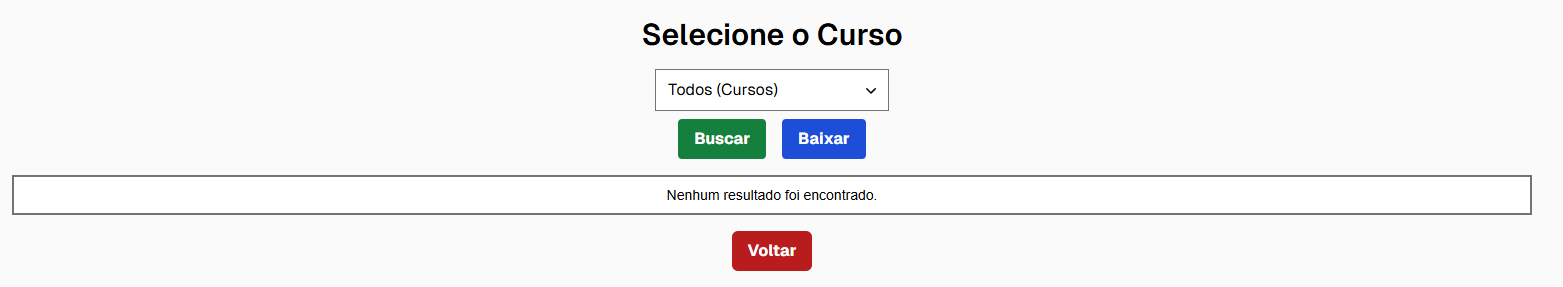
\includegraphics[width=1\textwidth]{Figuras/front-2.png}
    \caption*{Fonte: AUTOR (2025)}
    \label{fig_front_2}
\end{figure}

A Figura \ref{fig_front_2} apresenta a tela dos cursos, permitindo selecionar turmas e visualizar seus horários.

\begin{figure}[htb]
    \centering
    \caption{Tela dos cursos com cursos técnicos}
    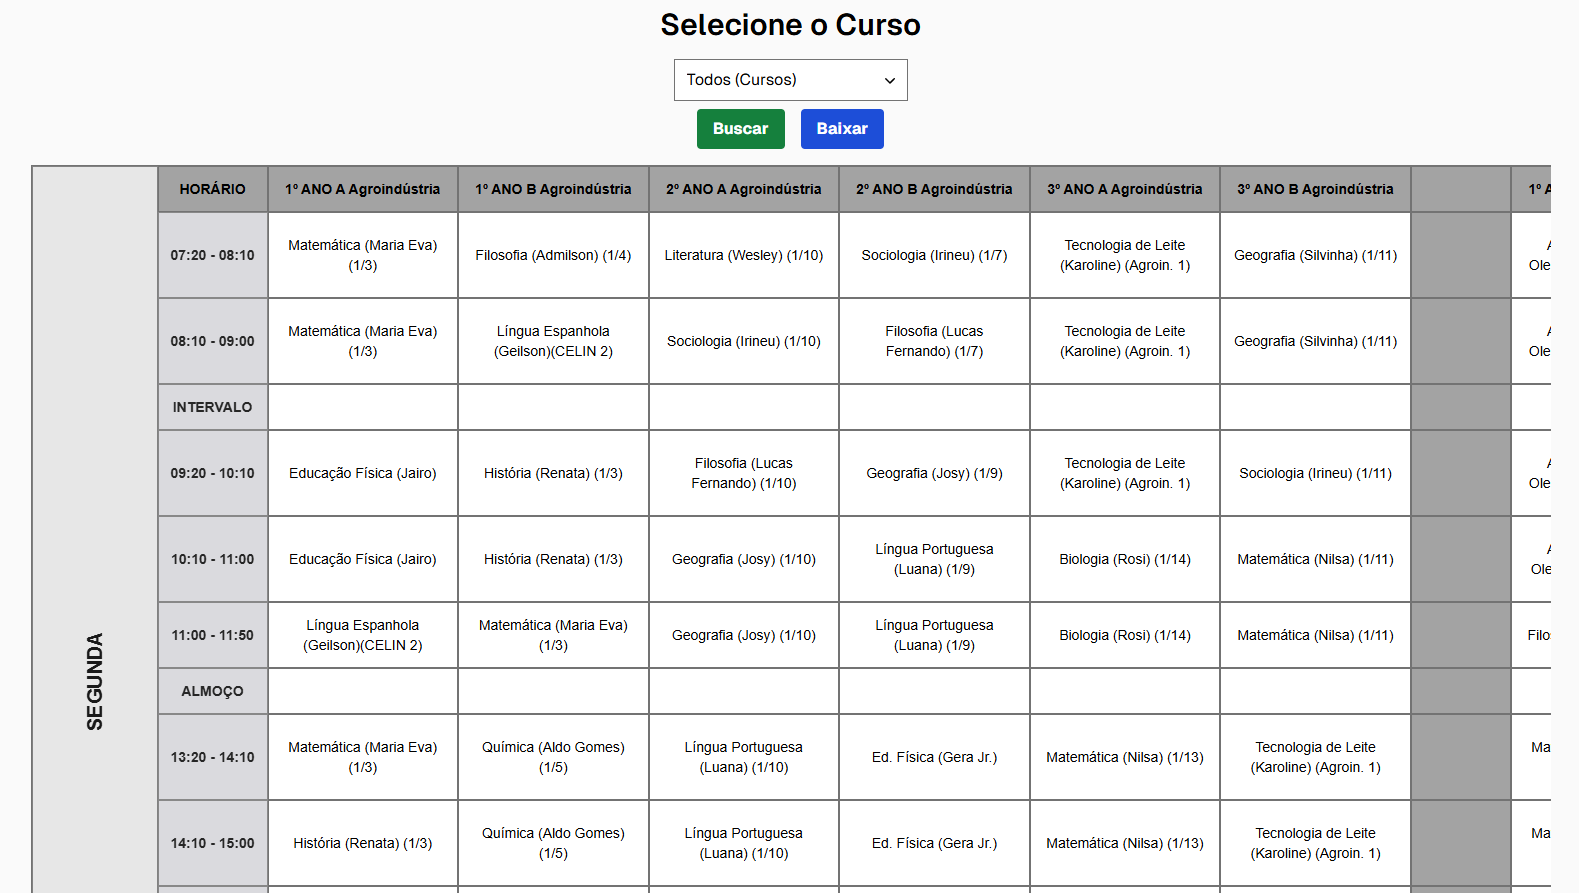
\includegraphics[width=1\textwidth]{Figuras/front-3.png}
    \caption*{Fonte: AUTOR (2025)}
    \label{fig_front_3}
\end{figure}

\begin{figure}[H]
    \centering
    \caption{Tela dos cursos com cursos superiores}
    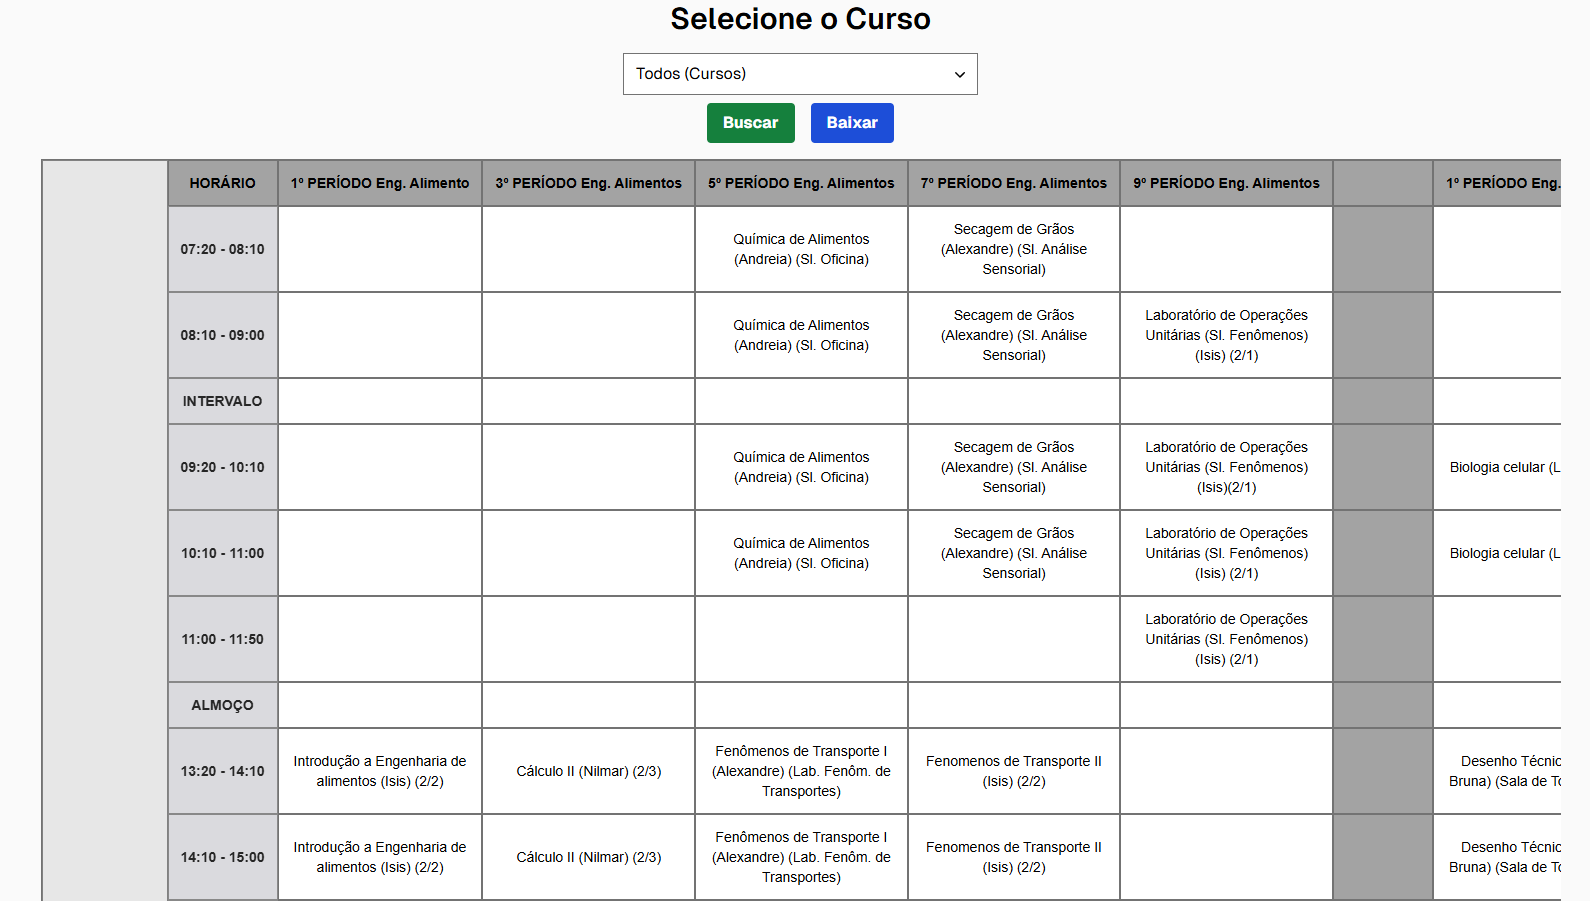
\includegraphics[width=1\textwidth]{Figuras/front-4.png}
    \caption*{Fonte: AUTOR (2025)}
    \label{fig_front_4}
\end{figure}

As Figuras \ref{fig_front_3} e \ref{fig_front_4} detalham, respectivamente, a exibição dos horários para cursos técnicos e superiores.

\begin{figure}[htb]
    \centering
    \caption{Tela dos professores}
    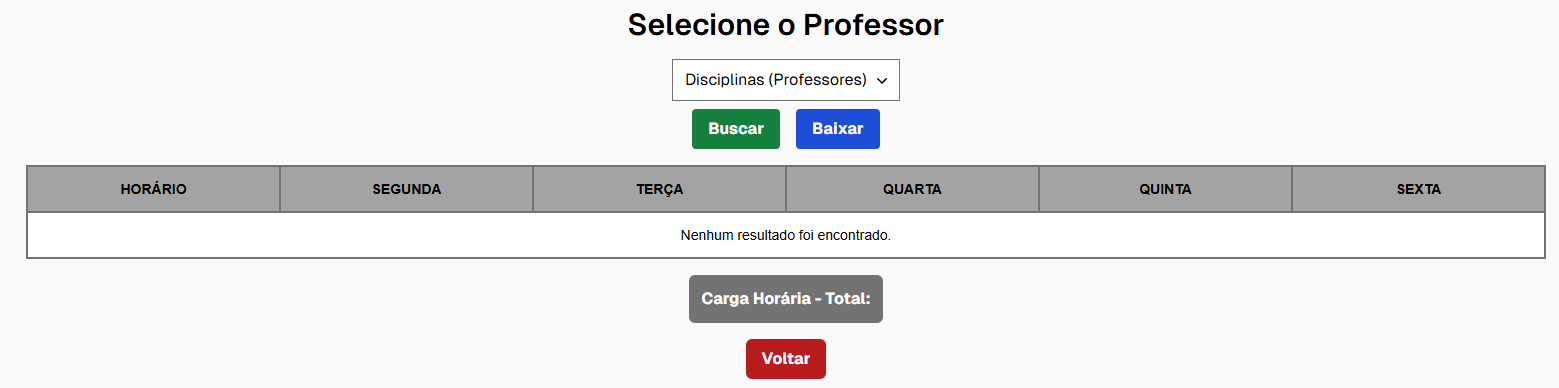
\includegraphics[width=1\textwidth]{Figuras/front-5.png}
    \caption*{Fonte: AUTOR (2025)}
    \label{fig_front_5}
\end{figure}

\begin{figure}[H]
    \centering
    \caption{Tela dos professores com um professor selecionado}
    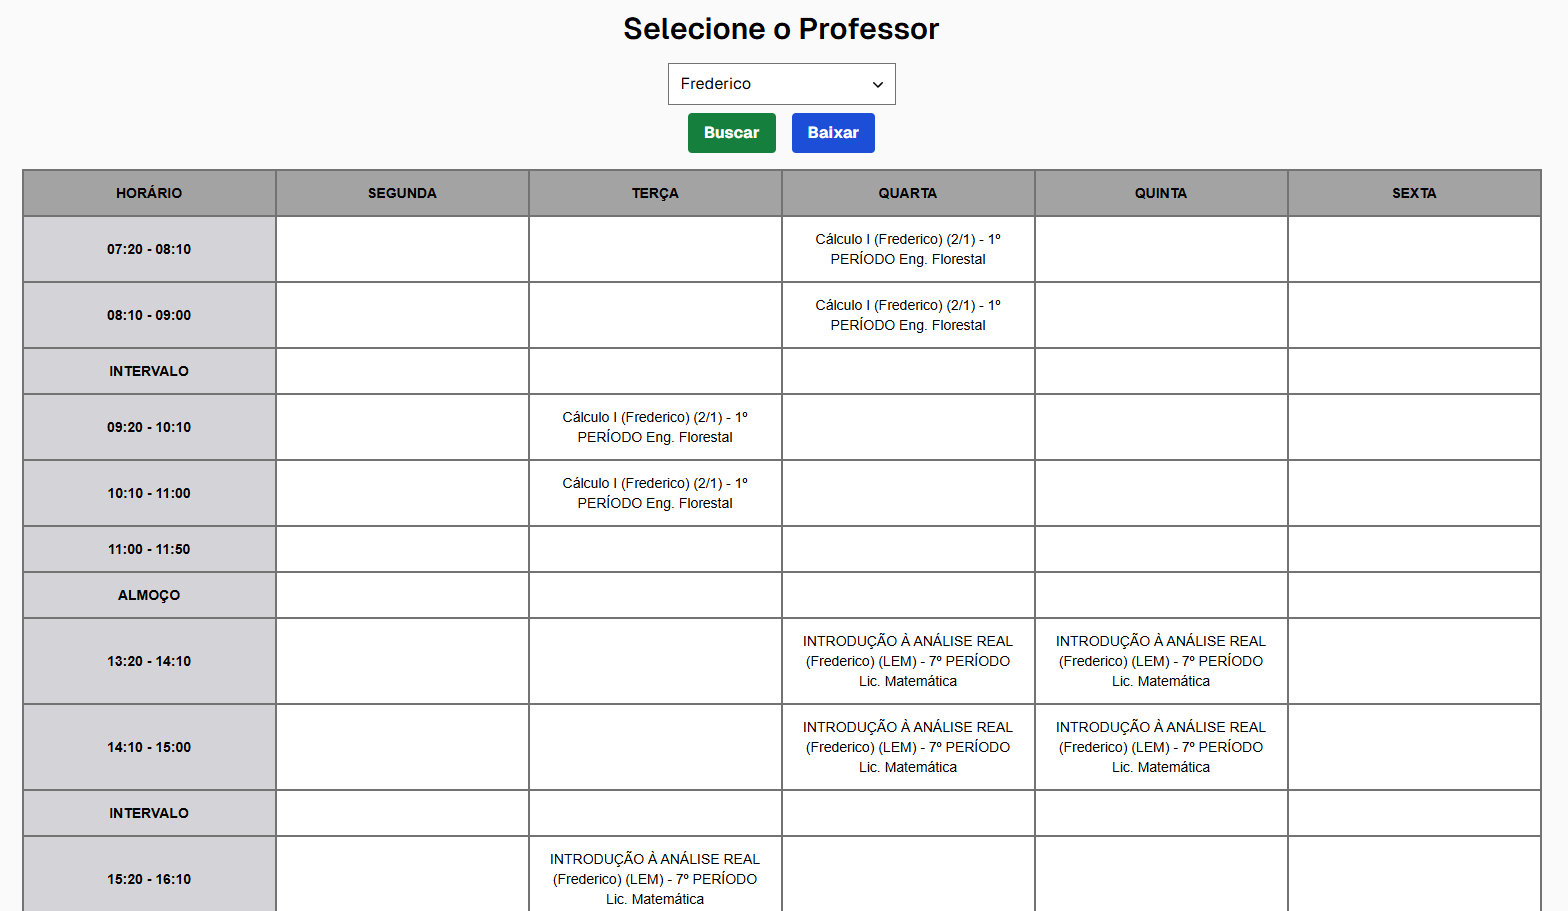
\includegraphics[width=1\textwidth]{Figuras/front-6.png}
    \caption*{Fonte: AUTOR (2025)}
    \label{fig_front_6}
\end{figure}

A Figura \ref{fig_front_5} ilustra a tela dos professores, enquanto a Figura \ref{fig_front_6} exibe um professor selecionado, com seus horários organizados.

\begin{figure}[H]
    \centering
    \caption{Tela das salas}
    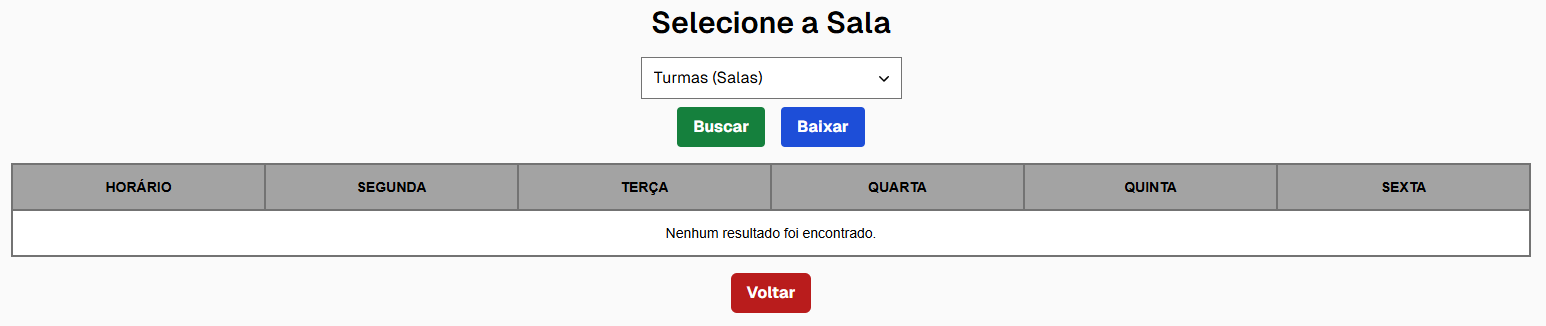
\includegraphics[width=1\textwidth]{Figuras/front-7.png}
    \caption*{Fonte: AUTOR (2025)}
    \label{fig_front_7}
\end{figure}

\begin{figure}[htb]
    \centering
    \caption{Tela das salas com uma sala selecionada}
    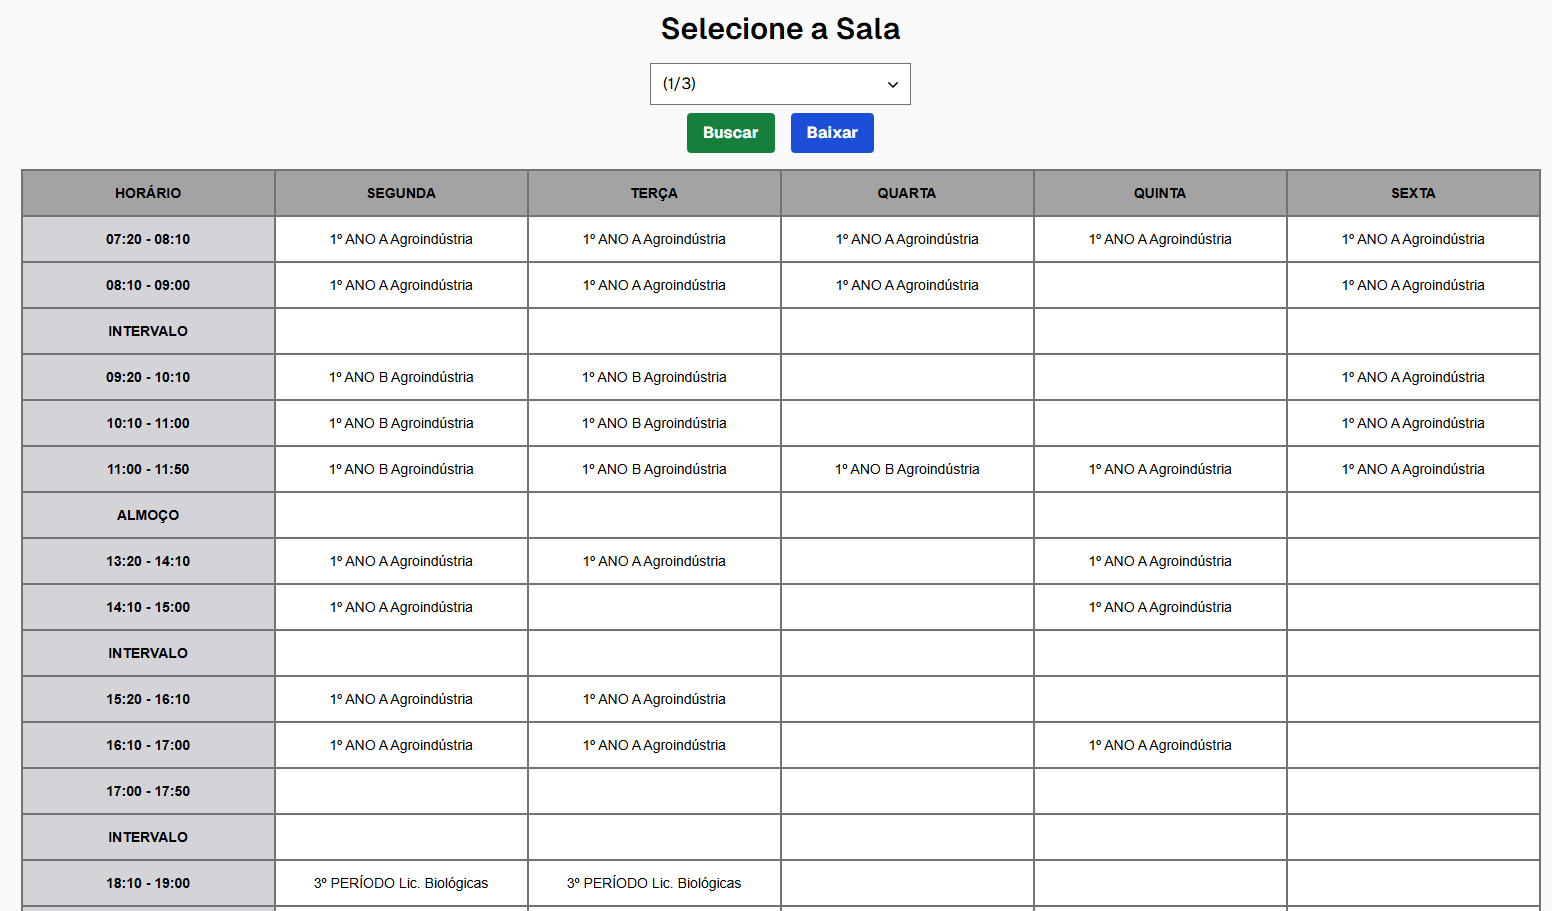
\includegraphics[width=1\textwidth]{Figuras/front-8.png}
    \caption*{Fonte: AUTOR (2025)}
    \label{fig_front_8}
\end{figure}

A Figura \ref{fig_front_7} apresenta a tela das salas e a Figura \ref{fig_front_8} mostra a visualização de uma sala específica com seu cronograma de uso.

\begin{figure}[htb]
    \centering
    \caption{Tela de login para acessar a tela de validação}
    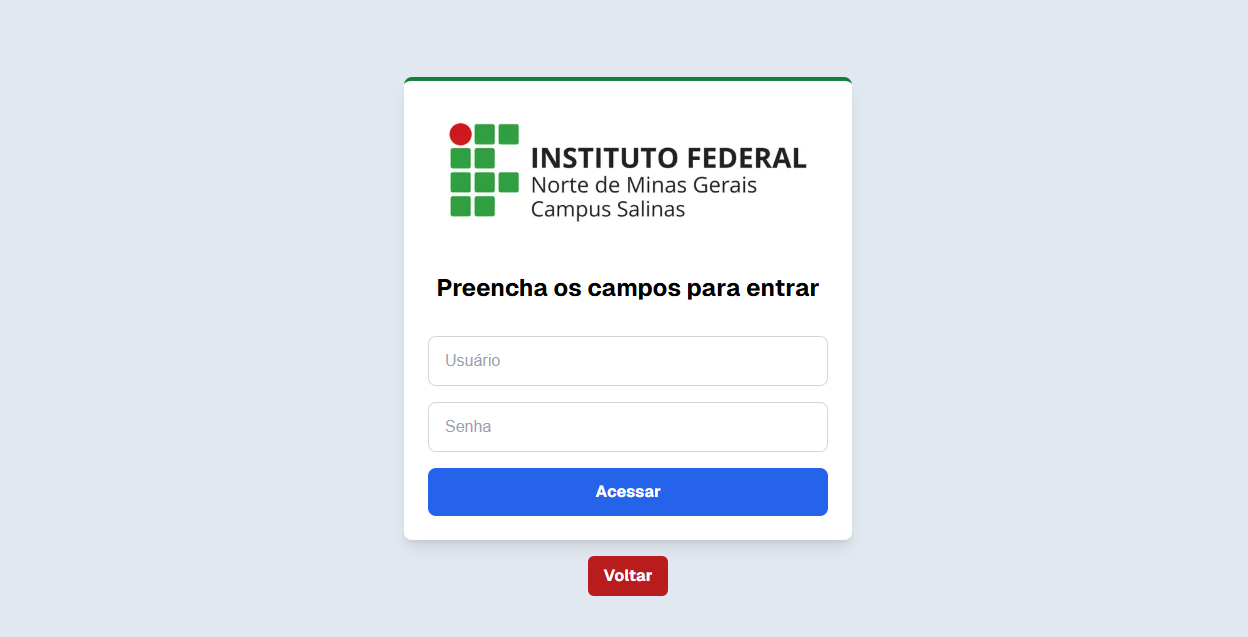
\includegraphics[width=1\textwidth]{Figuras/front-9.png}
    \caption*{Fonte: AUTOR (2025)}
    \label{fig_front_9}
\end{figure}

\begin{figure}[H]
    \centering
    \caption{Tela de validação}
    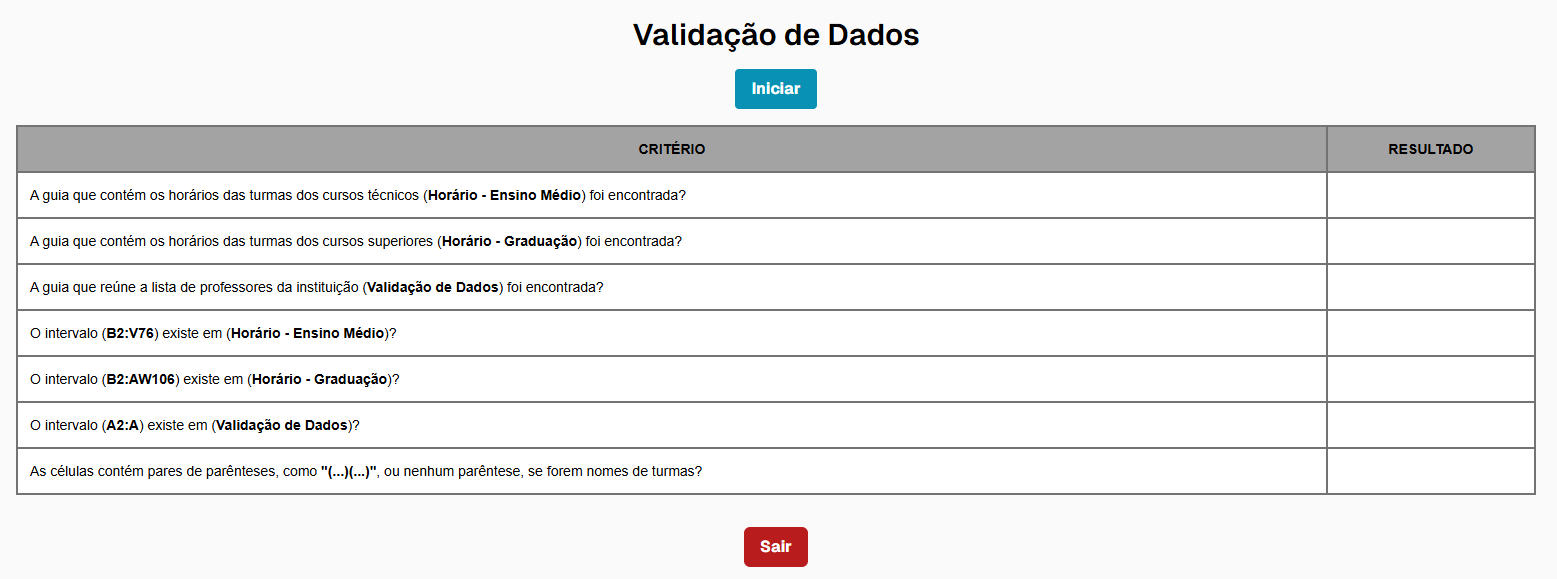
\includegraphics[width=1\textwidth]{Figuras/front-10.png}
    \caption*{Fonte: AUTOR (2025)}
    \label{fig_front_10}
\end{figure}

Já a Figura \ref{fig_front_9} traz a tela de login para acessar a área de validação de dados, e a Figura \ref{fig_front_10} mostra a tela de validação.

\begin{figure}[htb]
    \centering
    \caption{Sistema que exibe os locais do instituto}
    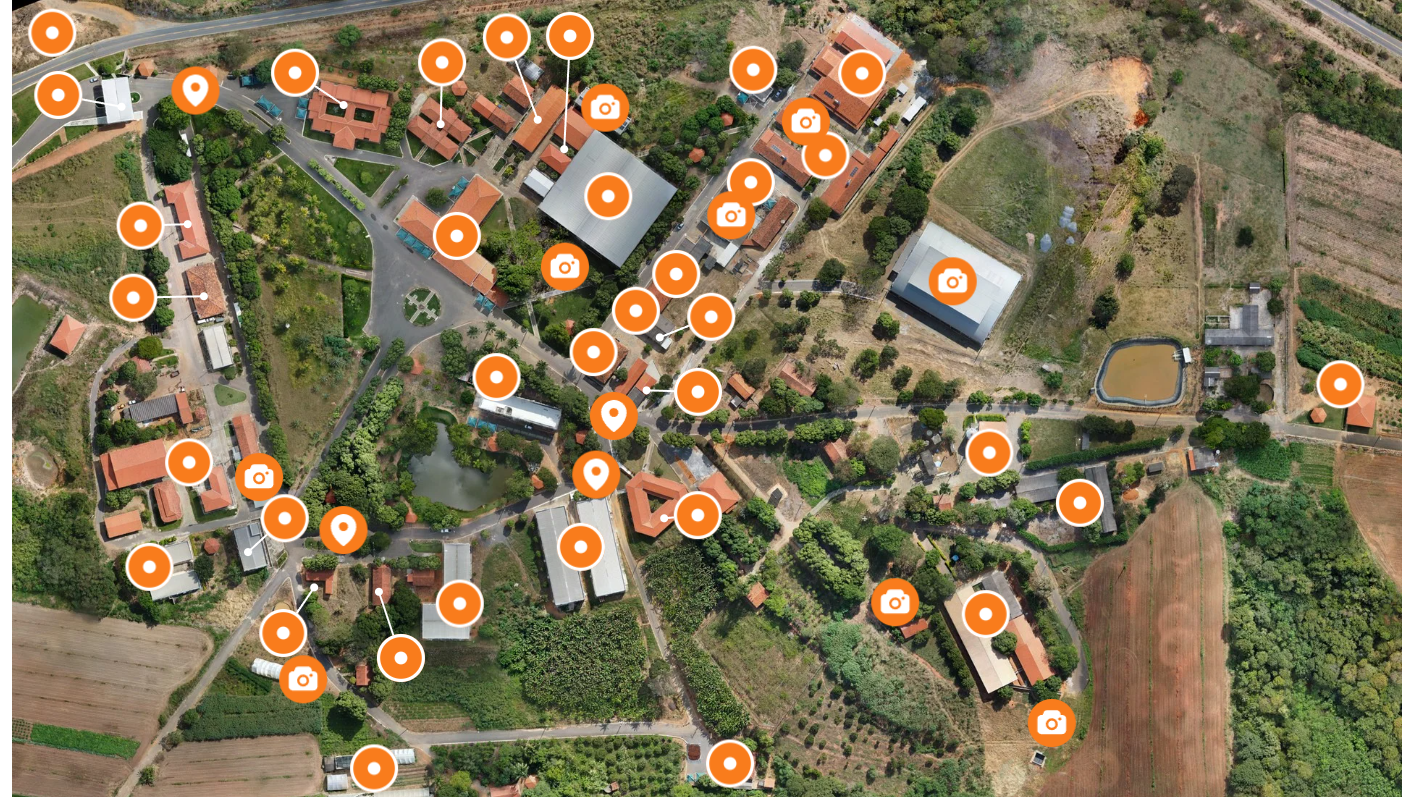
\includegraphics[width=1\textwidth]{Figuras/front-11.png}
    \caption*{Fonte: AUTOR (2025)}
    \label{fig_front_11}
\end{figure}

\begin{figure}[H]
    \centering
    \caption{Sistema de reserva de horários}
    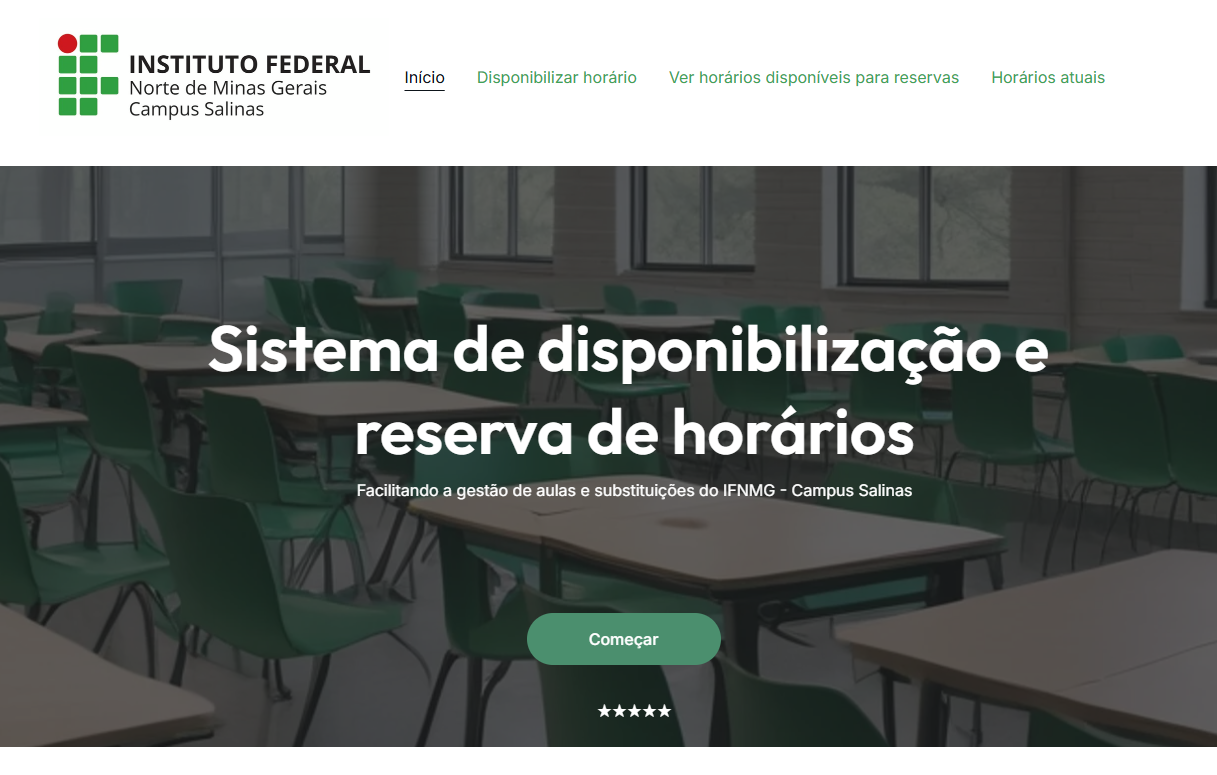
\includegraphics[width=1\textwidth]{Figuras/front-12.png}
    \caption*{Fonte: AUTOR (2025)}
    \label{fig_front_12}
\end{figure}

\begin{figure}[htb]
    \centering
    \caption{Sistema de gerenciamento de reserva de salas}
    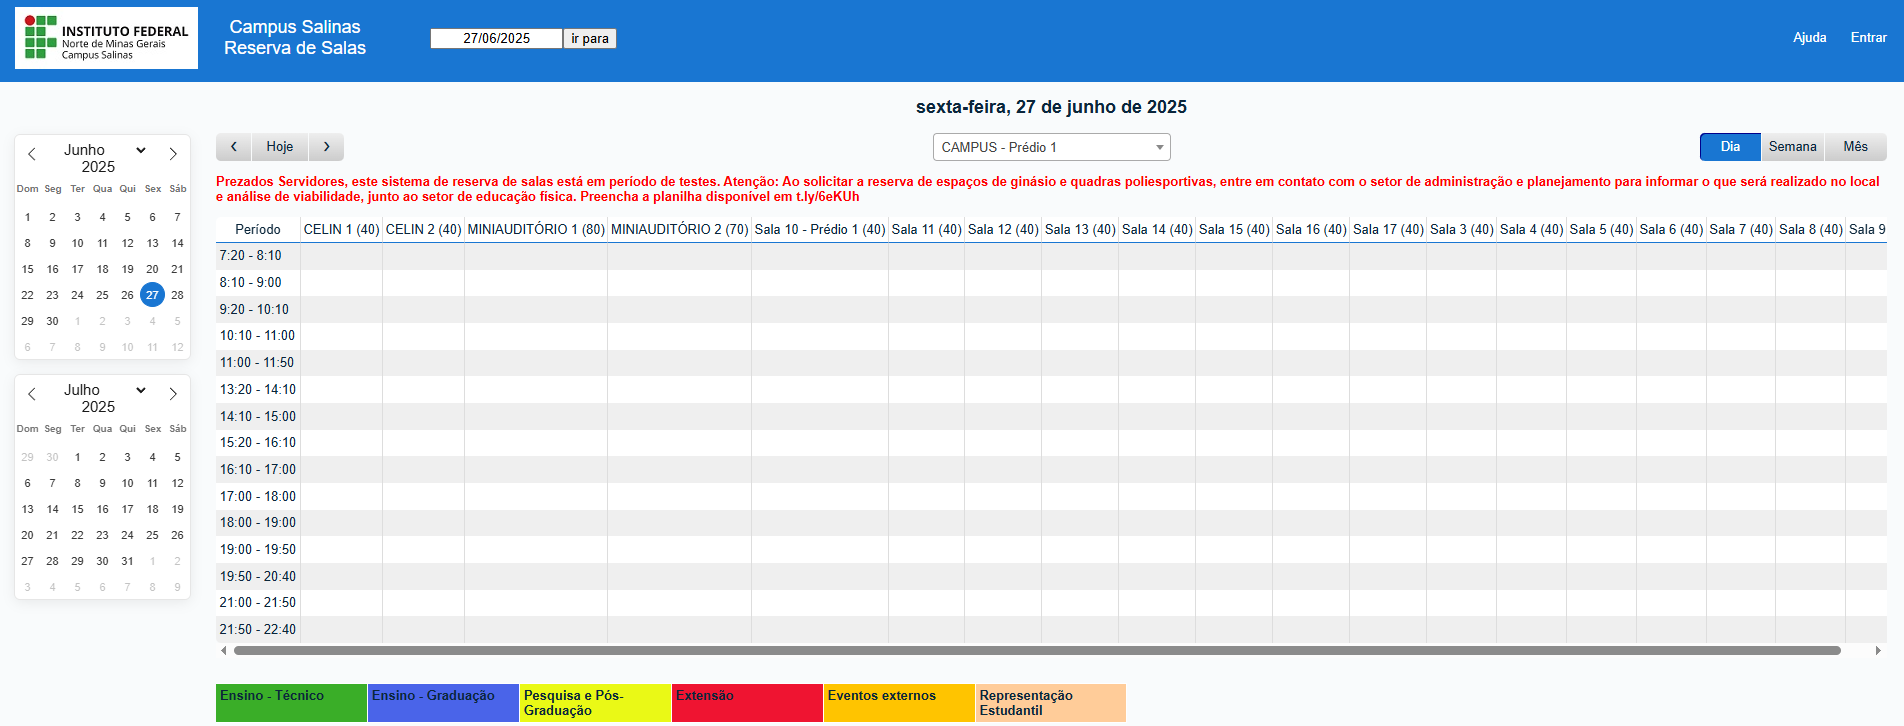
\includegraphics[width=1\textwidth]{Figuras/front-13.png}
    \caption*{Fonte: AUTOR (2025)}
    \label{fig_front_13}
\end{figure}

Por fim, as Figuras \ref{fig_front_11}, \ref{fig_front_12} e \ref{fig_front_13} ilustram os sistemas externos integrados à plataforma, incluindo a visualização de locais do instituto, o sistema de reserva de horários e o gerenciamento de reservas de salas. Esses sistemas, embora estejam acessíveis a partir da plataforma desenvolvida, não estão incluídos no escopo desse trabalho.

\subsection{Estrutura do Front-end}

A estrutura do front-end está organizada de forma modular, visando clareza, manutenção facilitada e reutilização de código. Na Figura \ref{fig_front_14}, destacam-se os principais elementos:

\begin{figure}[htb]
    \centering
    \caption{Estrutura do front-end}
    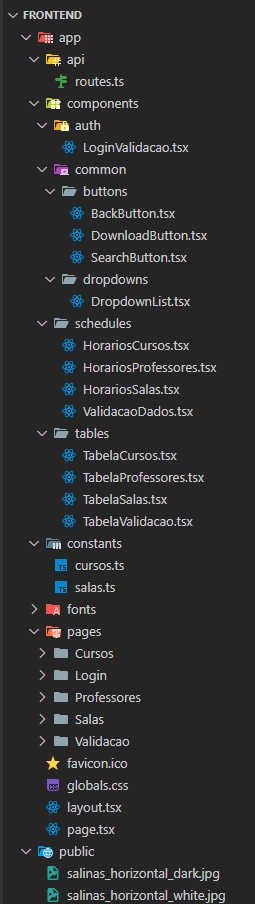
\includegraphics[width=0.3\textwidth]{Figuras/front-14.png}
    \caption*{Fonte: AUTOR (2025)}
    \label{fig_front_14}
\end{figure}

\begin{itemize}
    \item api: pasta responsável por buscar dados da planilha por meio de requisições, contando com o arquivo routes.ts para gerenciar essas chamadas.
    \item components: pasta que centraliza os componentes do sistema, subdividida em:
    \begin{itemize}
        \item auth: pasta responsável pelo controle de autenticação, incluindo o arquivo LoginValidacao.tsx, que verifica as credenciais de login antes de entrar na tela de validação.
        \item common: pasta destinada a componentes reutilizáveis, contendo:
        \begin{itemize}
            \item buttons: reúne botões de ação como BackButton.tsx (retorno), DownloadButton.tsx (download de tabelas) e SearchButton.tsx (busca de horários).
             \item dropdowns: responsável pelas listas suspensas, como o arquivo DropdownList.tsx, utilizado para seleção de cursos, professores ou salas.
        \end{itemize}
        \item schedules: pasta com componentes independentes para exibição de horários, como HorariosCursos.tsx, HorariosProfessores.tsx, HorariosSalas.tsx e ValidacaoDados.tsx.
        \item tables: pasta com componentes independentes para apresentação das tabelas com os dados, incluindo TabelaCursos.tsx, TabelaProfessores.tsx, TabelaSalas.tsx e TabelaValidacao.tsx.
    \end{itemize}
    \item constants: pasta responsável por definir as listas de cursos e salas disponíveis, armazenadas nos arquivos cursos.ts e salas.ts.
    \item pages: organiza as rotas da aplicação, com páginas específicas para cursos, professores, salas, login e validação.
    \item globals.css: arquivo de estilos globais aplicados em toda a interface.
    \item layout.tsx: define a estrutura geral de layout e permite a edição de metadados de forma centralizada.
    \item page.tsx: página inicial que exibe o menu principal com opções de botões de horários e outros serviços.
    \item public: pasta com imagens do logotipo institucional do IFNMG Campus Salinas, disponibilizadas tanto na versão padrão quanto na versão em preto e branco.
\end{itemize}

\subsection{Funcionalidades do Front-end}

\begin{itemize}
    \item Modo escuro: adapta automaticamente o tema da aplicação entre claro ou escuro, de acordo com a configuração do navegador, oferecendo maior conforto visual aos usuários. Conforme mostrado na Figura \ref{fig_front_15}.

    \begin{figure}[H]
        \centering
        \caption{Modo escuro}
        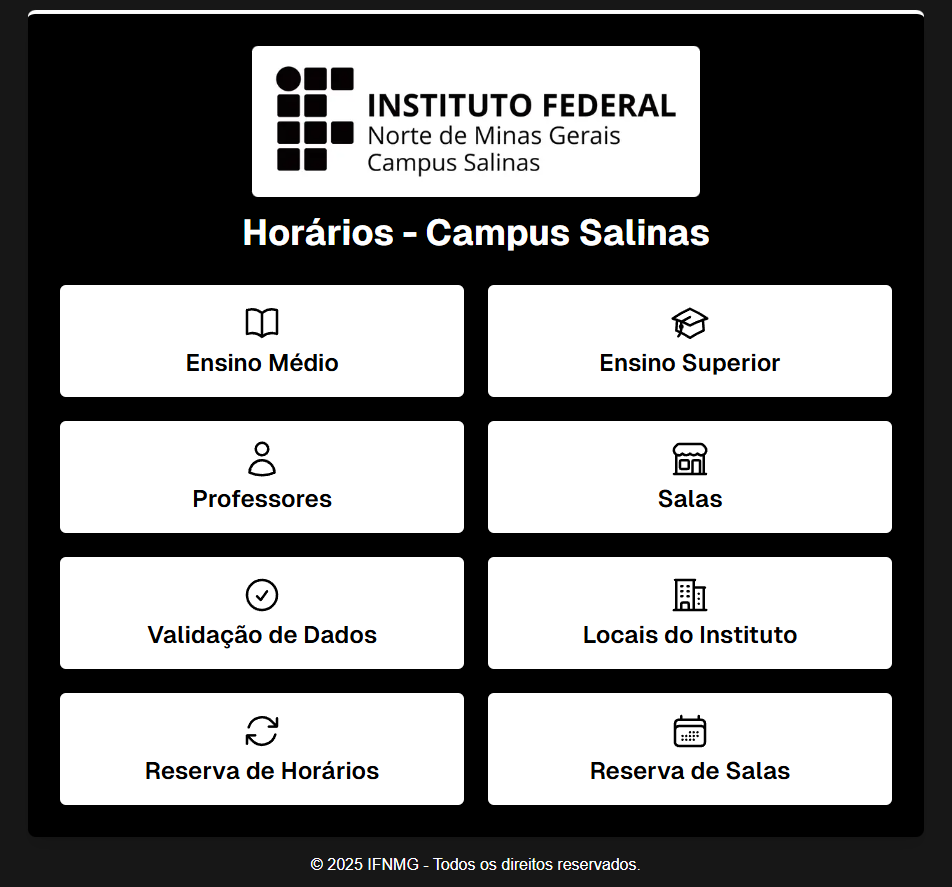
\includegraphics[width=0.9\textwidth]{Figuras/front-15.png}
        \caption*{Fonte: AUTOR (2025)}
        \label{fig_front_15}
    \end{figure}

    \item Responsividade: garante que a interface funcione bem tanto em dispositivos móveis quanto em desktops, mantendo a usabilidade e a organização dos elementos. Conforme mostrado na Figura \ref{fig_front_16}.

    \begin{figure}[H]
        \centering
        \caption{Responsividade}
        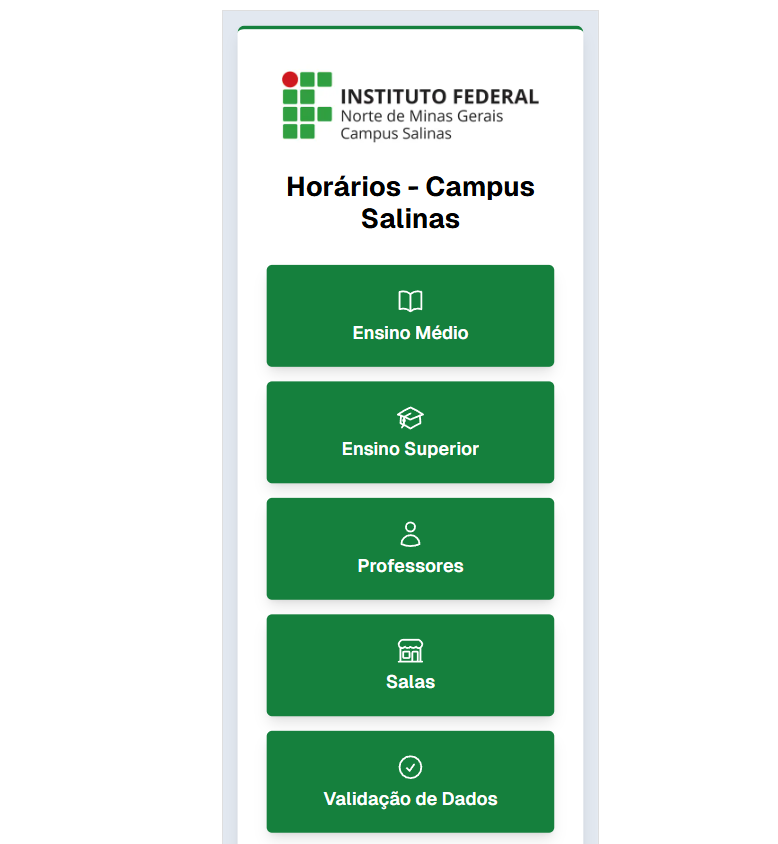
\includegraphics[width=0.3\textwidth]{Figuras/front-16.png}
        \caption*{Fonte: AUTOR (2025)}
        \label{fig_front_16}
    \end{figure}
    
    \item Busca de horários de cursos: possibilita consultar os horários dos cursos técnicos e superiores, exibindo os dias e horários de segunda a sexta-feira. Apresentado na Figura \ref{fig_front_17}.

    \begin{figure}[htb]
        \centering
        \caption{Busca de horários de cursos}
        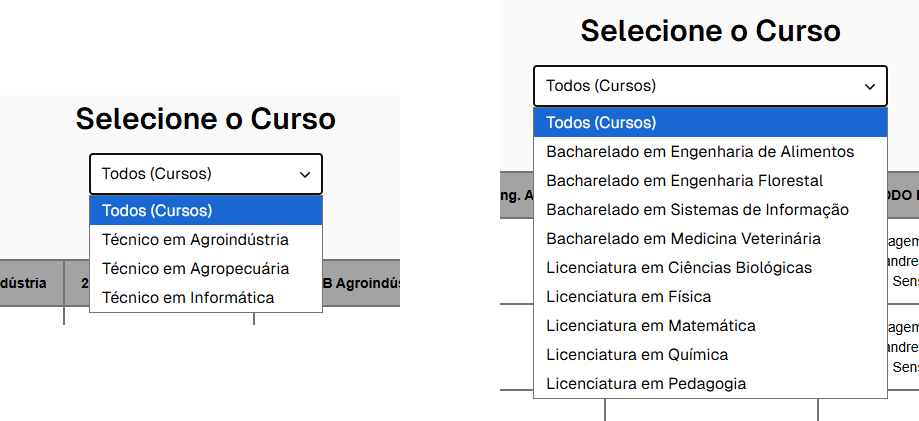
\includegraphics[width=0.7\textwidth]{Figuras/front-17.png}
        \caption*{Fonte: AUTOR (2025)}
        \label{fig_front_17}
    \end{figure}
    
    \item Busca de horários de professores: permite selecionar um professor em uma lista suspensa e visualizar os horários de segunda a sexta-feira. Ilustrado na Figura \ref{fig_front_18}.

    \begin{figure}[H]
        \centering
        \caption{Busca de horários de professores}
        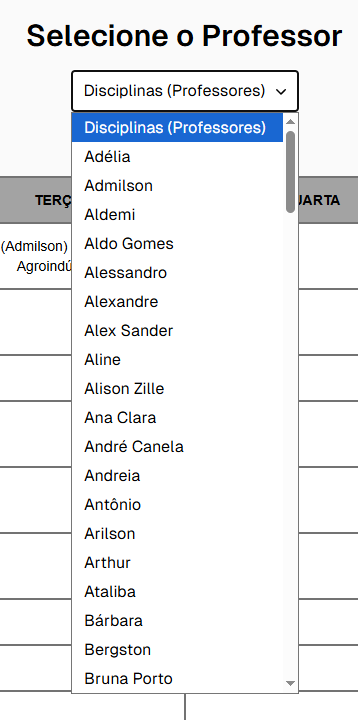
\includegraphics[width=0.25\textwidth]{Figuras/front-18.png}
        \caption*{Fonte: AUTOR (2025)}
        \label{fig_front_18}
    \end{figure}
    
    \item Busca de horários de salas: permite selecionar uma sala em uma lista suspensa e visualizar os horários de ocupação de segunda a sexta-feira. Conforme mostrado na Figura \ref{fig_front_19}.

    \begin{figure}[htb]
        \centering
        \caption{Busca de horários de salas}
        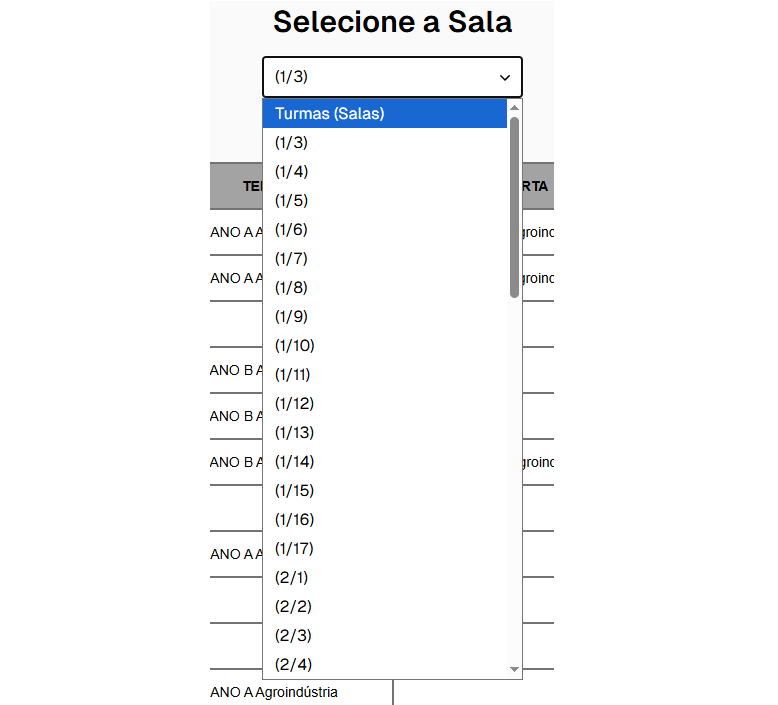
\includegraphics[width=0.25\textwidth]{Figuras/front-19.png}
        \caption*{Fonte: AUTOR (2025)}
        \label{fig_front_19}
    \end{figure}
    
    \item Download em PDF: permite o usuário salvar a tabela dos horários em um arquivo no formato PDF, facilitando o acesso offline às informações. Conforme mostrado na Figura \ref{fig_front_20}.

    \begin{figure}[htb]
        \centering
        \caption{Download em PDF}
        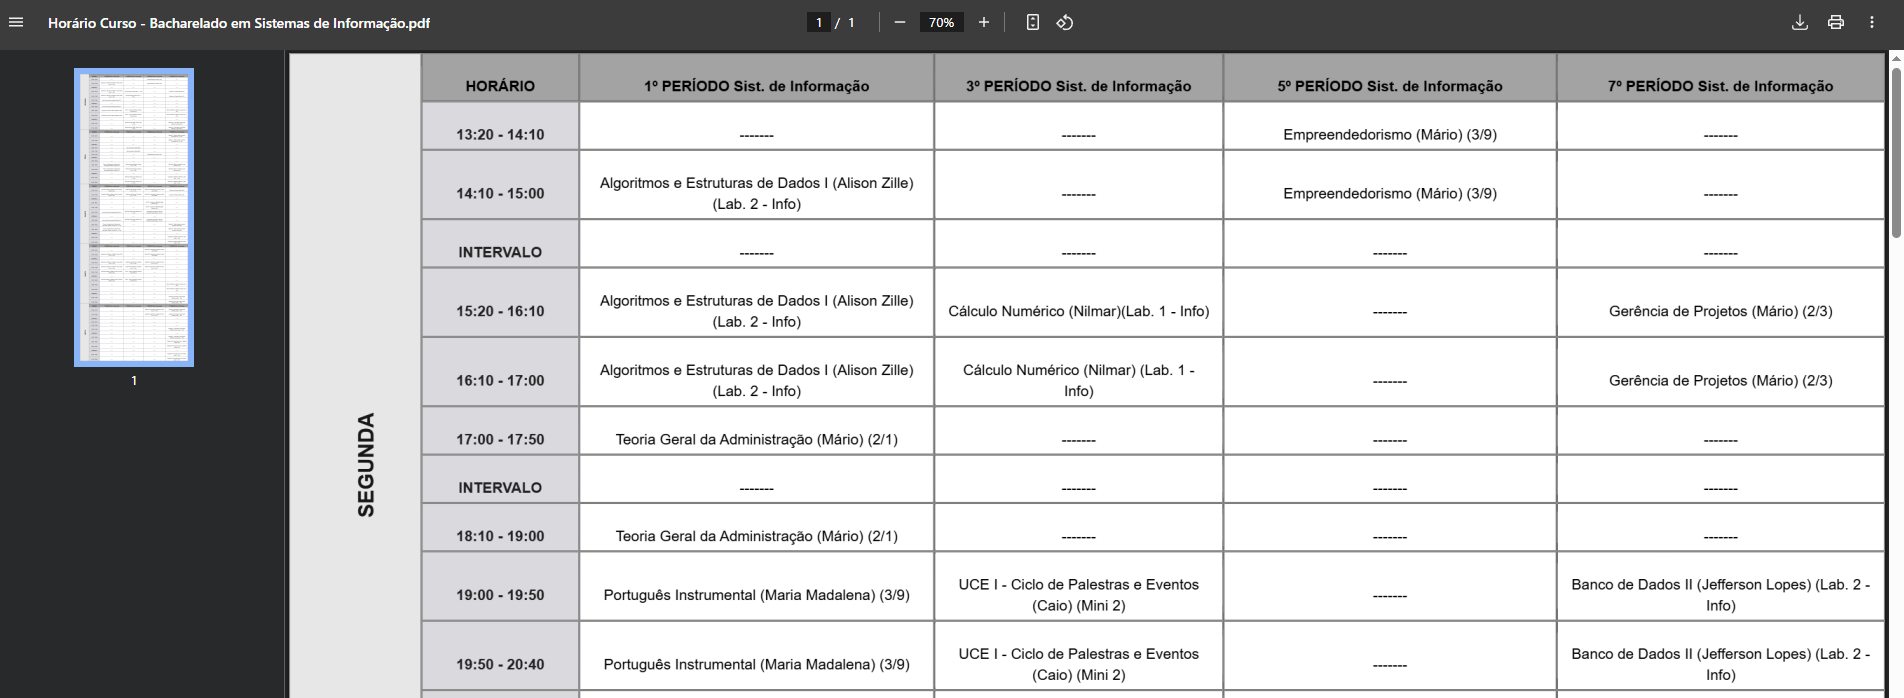
\includegraphics[width=0.9\textwidth]{Figuras/front-20.png}
        \caption*{Fonte: AUTOR (2025)}
        \label{fig_front_20}
    \end{figure}
    
    \item Tela de Login: restringe o acesso à tela de validação de dados apenas aos administradores, por meio de autenticação com usuário e senha. Ver Figura \ref{fig_front_21}.

    \begin{figure}[htb]
        \centering
        \caption{Tela de login com credenciais incorretas}
        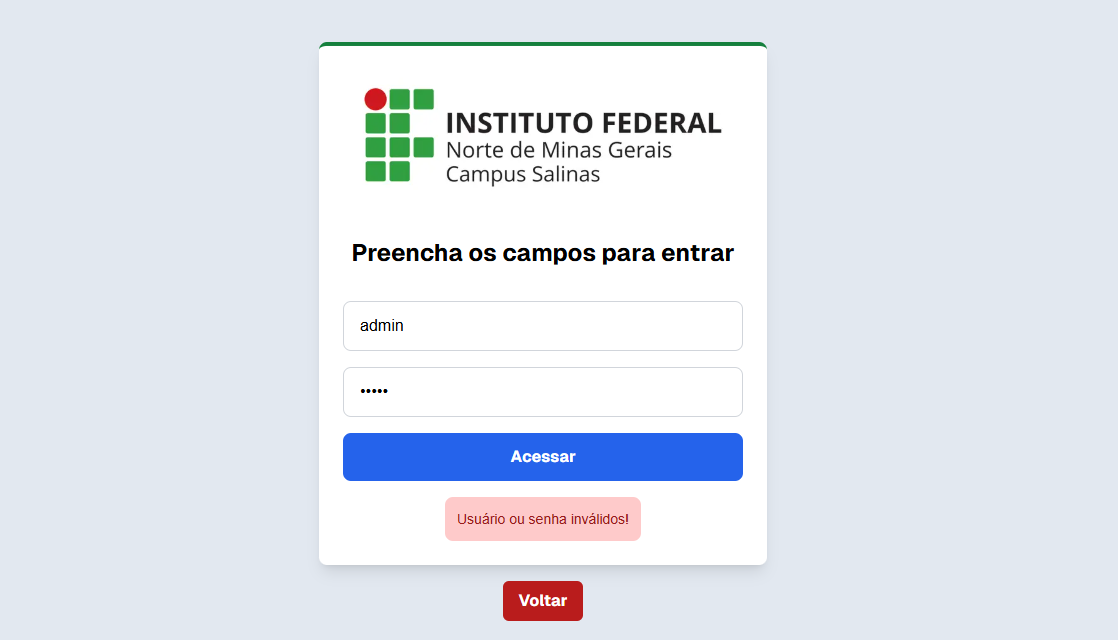
\includegraphics[width=0.8\textwidth]{Figuras/front-21.png}
        \caption*{Fonte: AUTOR (2025)}
        \label{fig_front_21}
    \end{figure}
    
    \item Tela de validação: exibe os resultados da verificação da planilha de horários, apresentando uma tabela com indicadores de conformidade (SIM ou NÃO) e validando:
    \begin{itemize}
        \item a presença das guias Horário - Ensino Médio, Horário - Graduação e Validação de Dados;
        \item a existência dos intervalos de células (B2:V76), (B2:AW106) e (A2:A);
        \item a formatação correta dos nomes, verificando se contêm os parênteses exigidos para turmas e professores. Se forem encontradas inconsistências, a tela exibe as células problemáticas, informando a guia, coluna e linha correspondentes. Ilustrado na Figura \ref{fig_front_22}.
    \end{itemize}

    \begin{figure}[htb]
        \centering
        \caption{Tela de Validação com resultados}
        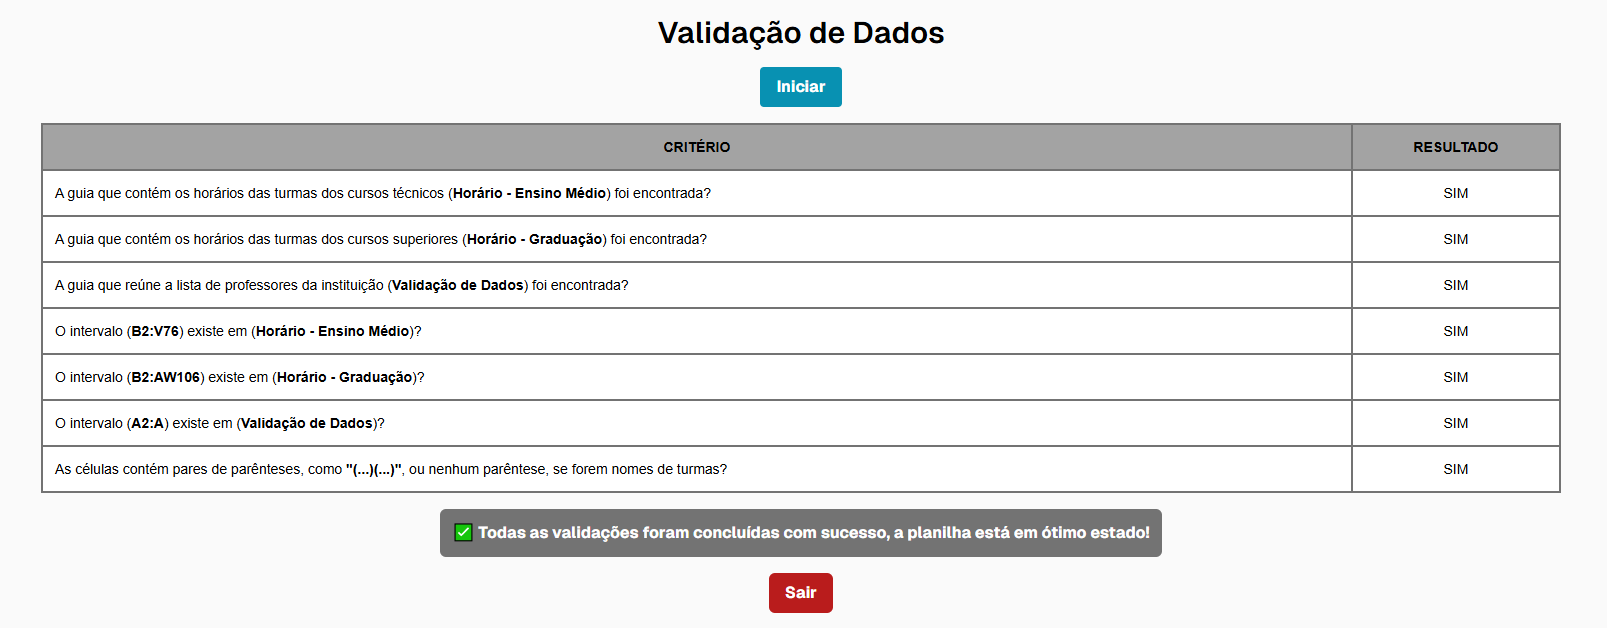
\includegraphics[width=1\textwidth]{Figuras/front-22.png}
        \caption*{Fonte: AUTOR (2025)}
        \label{fig_front_22}
    \end{figure}
\end{itemize}

\section{Back-end}

\subsection{Google Sheets como Banco de Dados}

O sistema utiliza duas planilhas hospedadas no Google Sheets. A primeira planilha contém duas guias com os horários acadêmicos e a uma guia com a lista dos professores disponíveis, conforme apresentado a seguir:

\begin{figure}[htb]
    \centering
    \caption{Horário - Ensino Médio}
    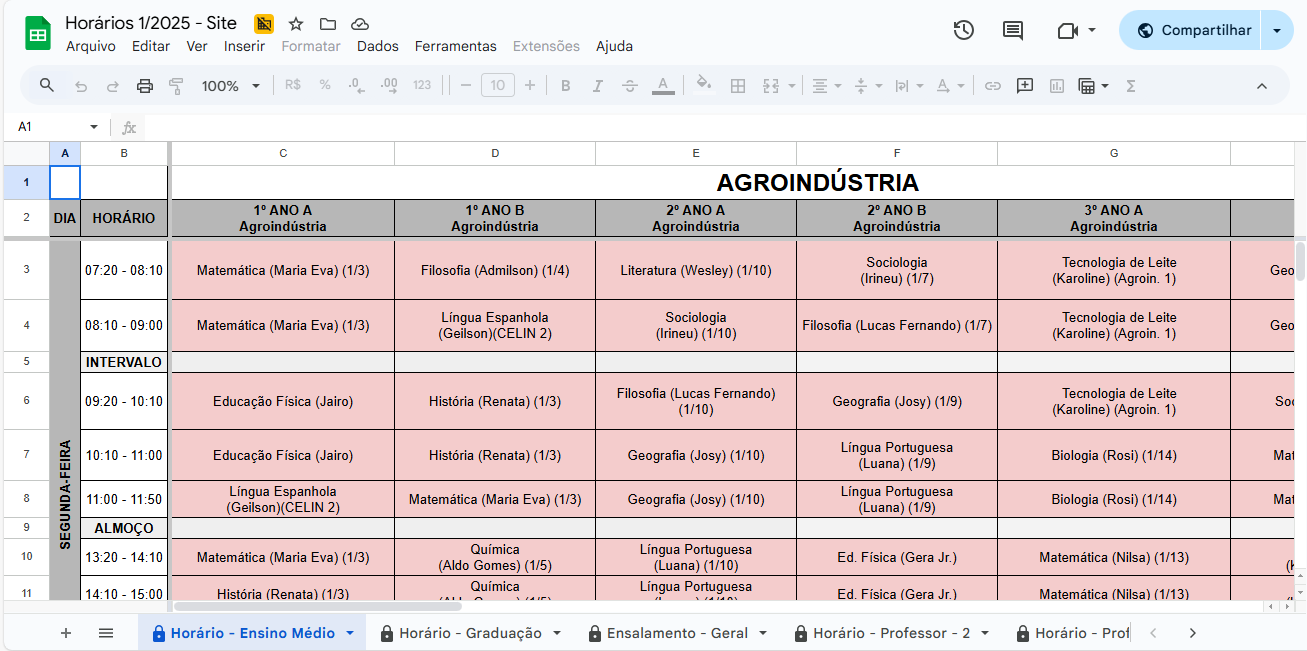
\includegraphics[width=0.9\textwidth]{Figuras/plan-1.png}
    \caption*{Fonte: AUTOR (2025)}
    \label{fig_plan_1}
\end{figure}

A Figura \ref{fig_plan_1} mostra a guia que contém os horários das turmas dos cursos técnicos, distribuídos no intervalo de células B2:V76.

\begin{figure}[htb]
    \centering
    \caption{Horário - Graduação}
    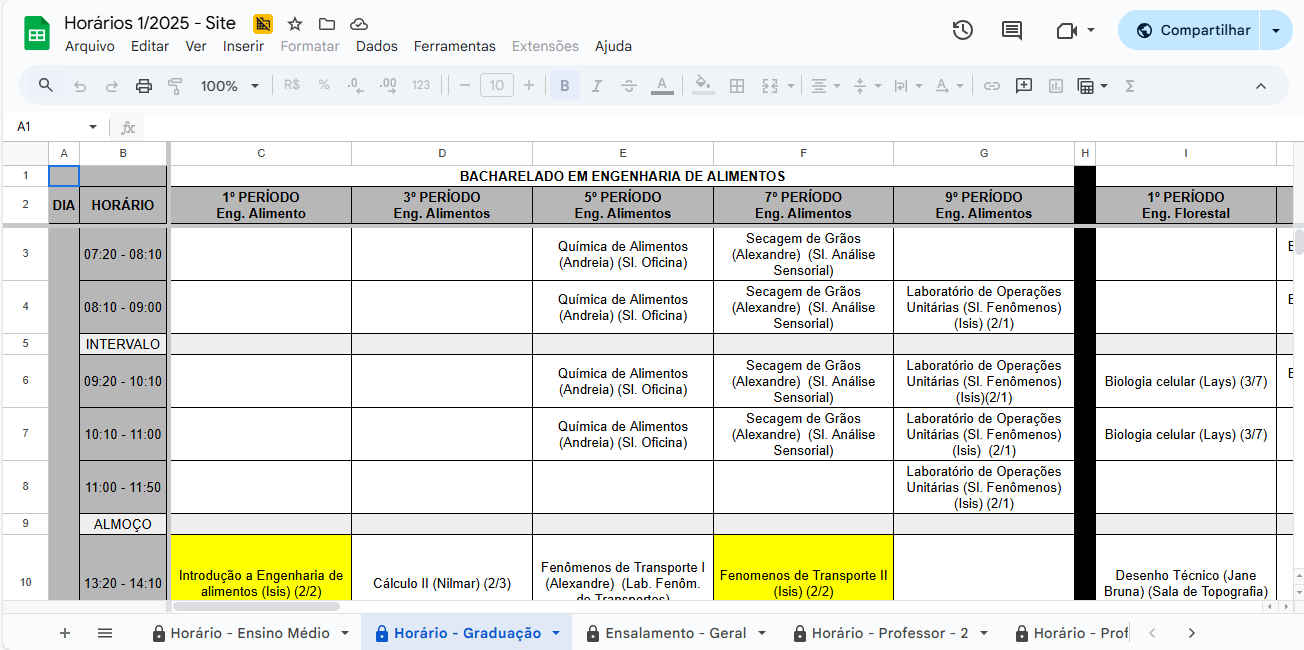
\includegraphics[width=0.9\textwidth]{Figuras/plan-2.png}
    \caption*{Fonte: AUTOR (2025)}
    \label{fig_plan_2}
\end{figure}

A Figura \ref{fig_plan_2} mostra a guia que contém os horários das turmas dos cursos superiores, distribuídos no intervalo de células B2:AW106.

\begin{figure}[htb]
    \centering
    \caption{Validação de Dados}
    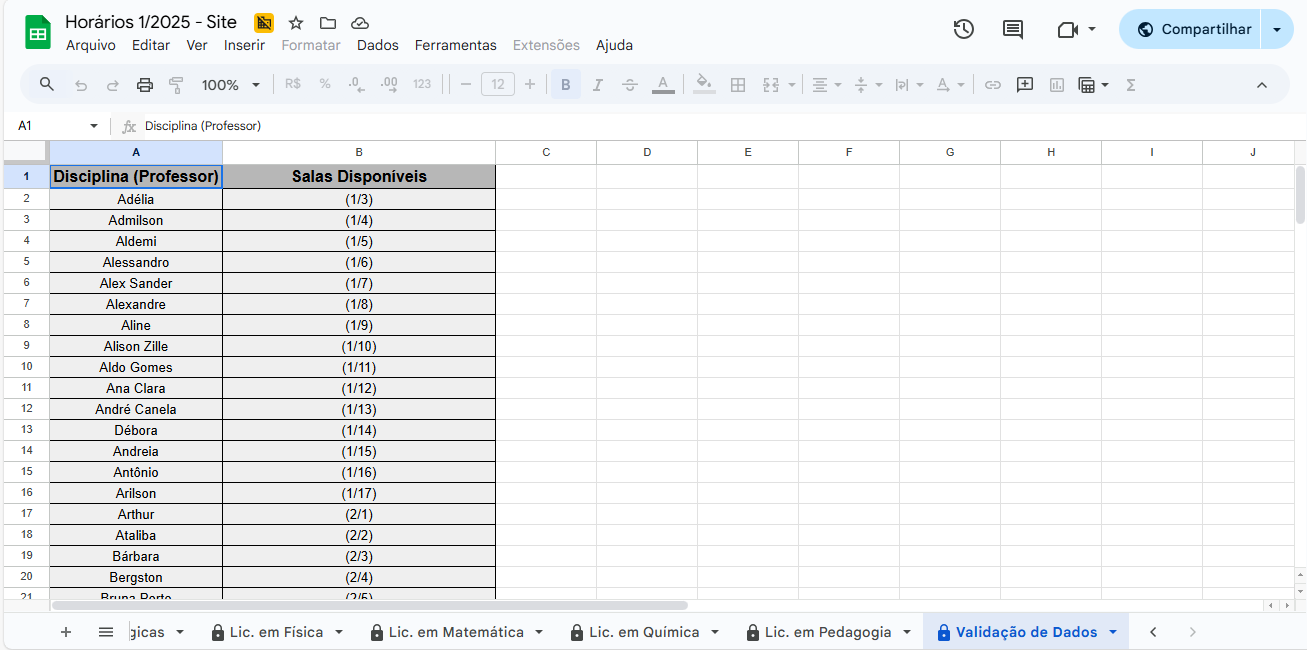
\includegraphics[width=0.9\textwidth]{Figuras/plan-3.png}
    \caption*{Fonte: AUTOR (2025)}
    \label{fig_plan_3}
\end{figure}

A Figura \ref{fig_plan_3}, mostra a guia que reúne a lista de professores da instituição, distribuídos no intervalo de células A2:A.

A segunda planilha contém uma guia com as credenciais de login necessárias para autenticação:

\begin{figure}[H]
    \centering
    \caption{Login}
    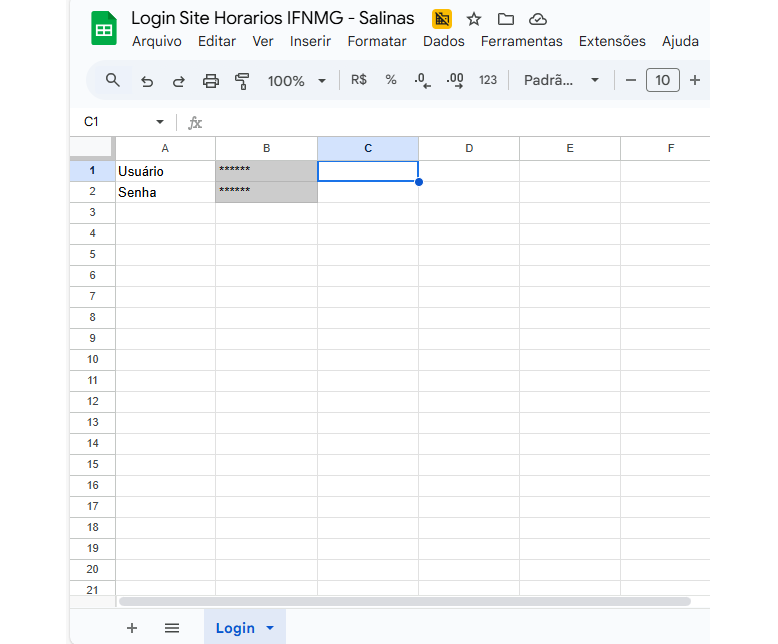
\includegraphics[width=0.9\textwidth]{Figuras/plan-4.png}
    \caption*{Fonte: AUTOR (2025)}
    \label{fig_plan_4}
\end{figure}

A Figura \ref{fig_plan_4} mostra a guia da planilha com as credenciais de login para acessar a tela de validação de dados, contendo os campos de usuário e senha, distribuídos no intervalo de células B1:B2.

\subsection{Desenvolvimento do Back-end}

O back-end foi desenvolvido utilizando o framework Spring Boot, escolhido por sua robustez, flexibilidade e ampla adoção no mercado. Essa tecnologia possibilitou integrar de forma segura a API do Google Sheets, garantindo a leitura dos dados necessários para o funcionamento da plataforma e enviando essas informações ao front-end de maneira estruturada e confiável. Todo o processo priorizou simplicidade na configuração e facilidade de manutenção, permitindo atender às demandas do projeto com eficiência. O código está disponível no repositório do projeto em \url{https://github.com/Tomaz5556/Horarios-IFNMG-Salinas/tree/main/backend}.

\subsection{Estrutura do Back-end}

A estrutura do back-end está organizada seguindo o padrão arquitetural MVC, o que favorece a separação de responsabilidades, facilita a manutenção e a evolução do sistema. Na Figura \ref{fig_back_1}, destacam-se os principais elementos do projeto:

\begin{figure}[htb]
    \centering
    \caption{Estrutura do back-end}
    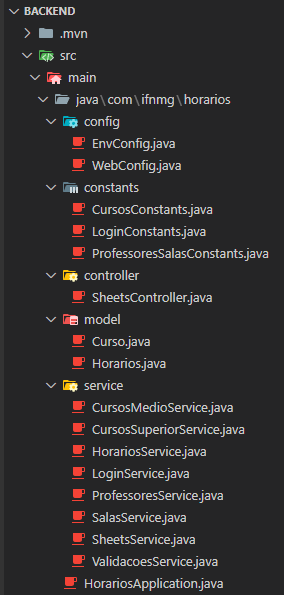
\includegraphics[width=0.4\textwidth]{Figuras/back-1.png}
    \caption*{Fonte: AUTOR (2025)}
    \label{fig_back_1}
\end{figure}

\begin{itemize}
    \item config: pasta responsável por armazenar classes de configuração do sistema, incluindo a EnvConfig.java, que define as variáveis de ambiente, e a WebConfig.java, responsável pelos ajustes de configuração da aplicação Spring Boot.
    \item constants: pasta responsável por centralizar valores fixos e listas utilizadas no sistema, contendo as classes CursosConstants.java, LoginConstants.java e ProfessoresSalasConstants.java, que mantêm os dados de cursos, professores, salas e credenciais de login.
    \item controller: pasta responsável por controlar as requisições recebidas e encaminhá-las para os serviços adequados, abrigando a classe SheetsController.java, que gerencia as rotas da aplicação.
    \item model: pasta responsável por definir as classes de domínio que representam a estrutura dos dados, como Curso.java e Horarios.java, que servem de modelo para a manipulação das informações obtidas do Google Sheets.
    \item service: pasta responsável por concentrar as regras de negócio e a comunicação com a API do Google Sheets, incluindo as classes CursosMedioService.java, CursosSuperiorService.java, HorariosService.java, LoginService.java, ProfessoresService.java, SalasService.java, SheetsService.java e ValidacoesService.java.
    \item HorariosApplication.java: arquivo inicializador da aplicação Spring Boot, responsável por executar o sistema e carregar todas as configurações necessárias para o funcionamento da plataforma.
\end{itemize}

\subsection{Funcionalidades do Back-end}

\begin{itemize}
    \item Estabelecer a conexão segura com a API do Google Sheets para coletar os dados das planilhas utilizadas como banco de dados. Essa função é executada pela classe SheetsService, que gerencia a integração entre o back-end e o serviço do Google, possibilitando o acesso dinâmico e estruturado às informações necessárias para o funcionamento da plataforma.
    
    \begin{figure}[H]
        \centering
        \caption{SheetsService.java}
        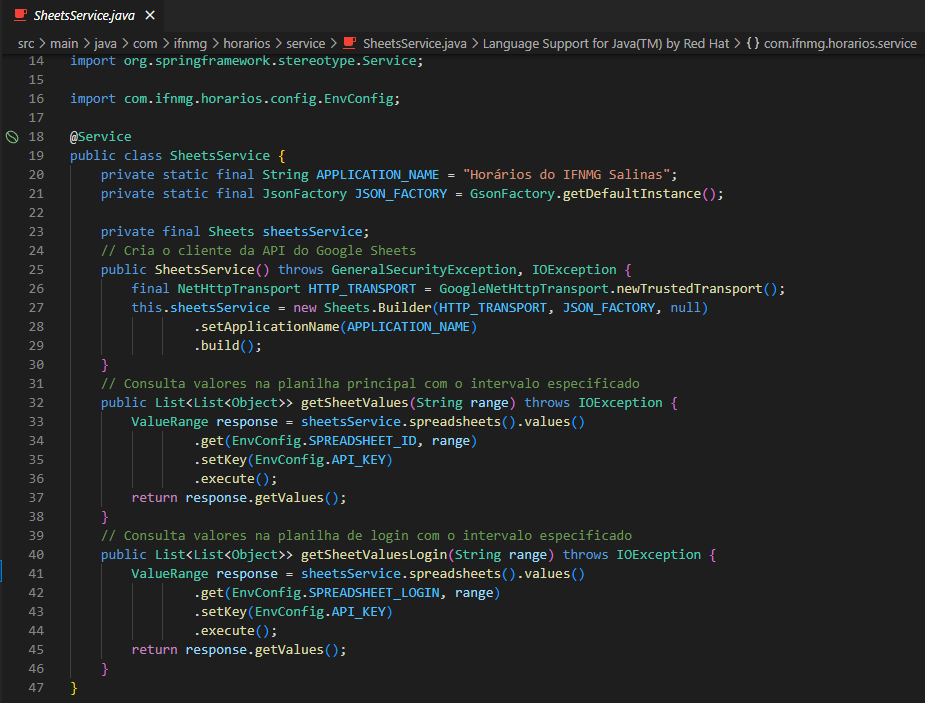
\includegraphics[width=1\textwidth]{Figuras/back-2.png}
        \caption*{Fonte: AUTOR (2025)}
        \label{fig_back_2}
    \end{figure}
    
    A Figura \ref{fig_back_2} mostra a classe SheetsService.java. A seguir, estão descritas suas principais funcionalidades:

    \begin{itemize}
        \item \textbf{Constantes}: APPLICATION\_NAME e JSON\_FACTORY são utilizadas para configurar a instância da API do Google Sheets. O nome da aplicação é definido para identificação no console da API, e o JsonFactory especifica o formato de serialização dos dados trafegados entre o back-end e o serviço do Google.
        \item \textbf{Construtor SheetsService()}: Responsável por configurar a instância do cliente da API do Google Sheets, que é armazenada no atributo sheetsService. Para isso, é utilizada uma conexão segura, criada com GoogleNetHttpTransport, garantindo uma comunicação autenticada e confiável entre o sistema e a API.
        \item \textbf{Método getSheetValues(String range)}: Lê os dados da planilha principal, onde estão os horários acadêmicos, com base no intervalo informado. O método utiliza duas variáveis de ambiente:
        \begin{itemize}
            \item \textit{EnvConfig.SPREADSHEET\_ID}: ID da planilha com os horários acadêmicos.
            \item \textit{EnvConfig.API\_KEY}: chave de acesso à API do Google Sheets.
        \end{itemize}
        \item \textbf{Método getSheetValuesLogin(String range)}: Realiza a leitura de dados da planilha de login, usada na tela de validação de dados. Utiliza como base:
        \begin{itemize}
            \item \textit{EnvConfig.SPREADSHEET\_LOGIN}: ID da planilha com as credenciais de login.
            \item \textit{EnvConfig.API\_KEY}: mesma chave usada no método anterior.
        \end{itemize}
    \end{itemize}

    \item Disponibilizar endpoints REST para consulta de horários de cursos, professores, salas e resultados de validação de dados, assegurando respostas padronizadas e consistentes. Essa funcionalidade é implementada na classe SheetsController, que organiza e define as rotas de acesso dos dados. As rotas são definidas exclusivamente com o método GET, uma vez que o sistema realiza apenas operações de leitura, sem modificar os dados. Cada rota é mapeada para um método específico do controller, responsável por retornar as informações de forma estruturada por meio do objeto ResponseEntity. A seguir, são descritos os principais endpoints da aplicação.

    \begin{figure}[htb]
        \centering
        \caption{Endpoint de consulta dos horários dos cursos técnicos}
        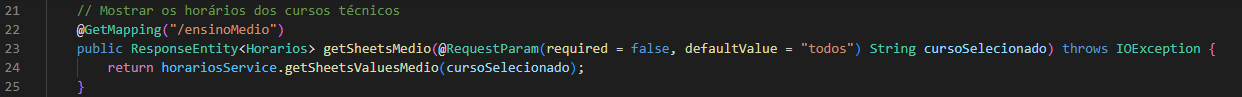
\includegraphics[width=1\textwidth]{Figuras/back-3.png}
        \caption*{Fonte: AUTOR (2025)}
        \label{fig_back_3}
    \end{figure}

    O objetivo do endpoint apresentado na Figura \ref{fig_back_3} é retornar os horários dos cursos técnicos. O parâmetro utilizado é cursoSelecionado, que é opcional e, por padrão, assume o valor "todos". Tendo isso como referência, o sistema consulta os dados na planilha e os retorna de forma organizada dentro de um objeto Horarios com os horários de todos os cursos técnicos ou de um curso técnico específico.

    \begin{figure}[htb]
        \centering
        \caption{Endpoint de consulta dos horários dos cursos superiores}
        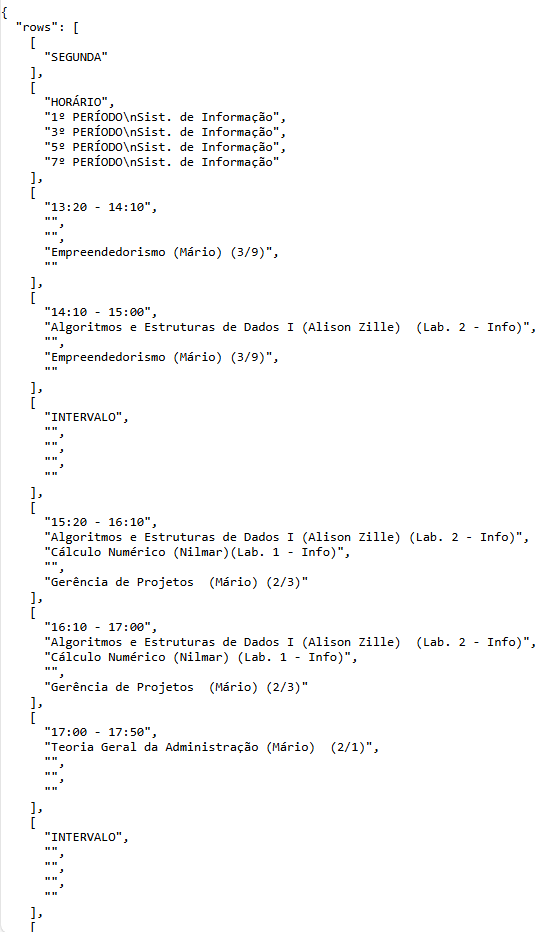
\includegraphics[width=1\textwidth]{Figuras/back-4.png}
        \caption*{Fonte: AUTOR (2025)}
        \label{fig_back_4}
    \end{figure}

    O objetivo do endpoint apresentado na Figura \ref{fig_back_4} é retornar os horários dos cursos superiores. O parâmetro utilizado é cursoSelecionado, que é opcional e, por padrão, assume o valor "todos". Tendo isso como referência, o sistema consulta os dados na planilha e os retorna de forma organizada dentro de um objeto Horarios com os horários de todos os cursos superiores ou de um curso superior específico.

    \begin{figure}[H]
        \centering
        \caption{Endpoint de consulta dos horários dos professores}
        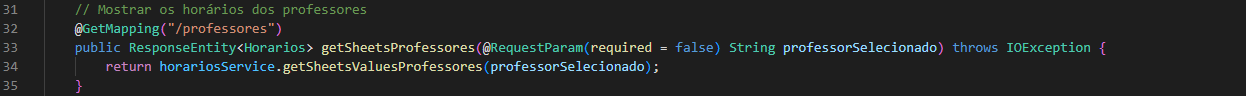
\includegraphics[width=1\textwidth]{Figuras/back-5.png}
        \caption*{Fonte: AUTOR (2025)}
        \label{fig_back_5}
    \end{figure}

    Conforme ilustrado na Figura \ref{fig_back_5}, o objetivo do endpoint é retornar os horários dos professores. O parâmetro professorSelecionado é opcional e pode ser deixado em branco. Com base nisso, o sistema consulta os dados na planilha e os retorna de forma organizada dentro de um objeto Horarios com os horários de um professor específico.

    \begin{figure}[htb]
        \centering
        \caption{Endpoint de consulta dos horários de ocupação das salas}
        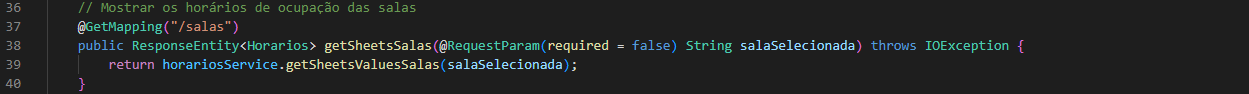
\includegraphics[width=1\textwidth]{Figuras/back-6.png}
        \caption*{Fonte: AUTOR (2025)}
        \label{fig_back_6}
    \end{figure}

    Conforme ilustrado na Figura \ref{fig_back_6}, o objetivo do endpoint é retornar os horários de ocupação das salas. O parâmetro salaSelecionada é opcional e pode ser deixado em branco. Com base nisso, o sistema consulta os dados na planilha e os retorna de forma organizada dentro de um objeto Horarios com os horários de ocupação de uma sala específica.

    \begin{figure}[htb]
        \centering
        \caption{Endpoint de consulta das permissões para ver validação da planiha}
        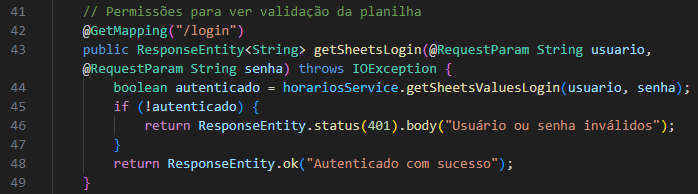
\includegraphics[width=1\textwidth]{Figuras/back-7.png}
        \caption*{Fonte: AUTOR (2025)}
        \label{fig_back_7}
    \end{figure}

    Como mostrado na Figura \ref{fig_back_7}, o objetivo do endpoint é validar as credenciais de acesso informadas. Os parâmetros obrigatórios são usuario e senha. Com essas informações, o sistema realiza a autenticação e retorna uma mensagem com o status correspondente, sendo 200 em caso de sucesso ou 401 não autorizado caso as credenciais estejam incorretas.

    \begin{figure}[H]
        \centering
        \caption{Endpoint de consulta para validar dados da planilha}
        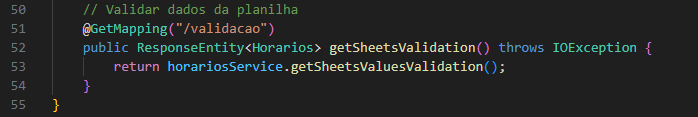
\includegraphics[width=1\textwidth]{Figuras/back-8.png}
        \caption*{Fonte: AUTOR (2025)}
        \label{fig_back_8}
    \end{figure}

    Conforme mostrado na Figura \ref{fig_back_8}, o objetivo do endpoint é retornar os resultados da validação dos dados da planilha de horários. Nenhum parâmetro é necessário para a execução da requisição. Ao ser acionado, o sistema analisa a planilha e responde com um objeto Horarios contendo eventuais inconsistências ou erros detectados durante o processo de validação.
\end{itemize}

\section{Deploy}

O front-end foi hospedado na plataforma Vercel, permitindo a disponibilização da interface do usuário com alta performance e integração contínua, como mostrado na Figura \ref{fig_deploy_1}.

\begin{figure}[htb]
    \centering
    \caption{Deploy do front-end da plataforma na Vercel}
    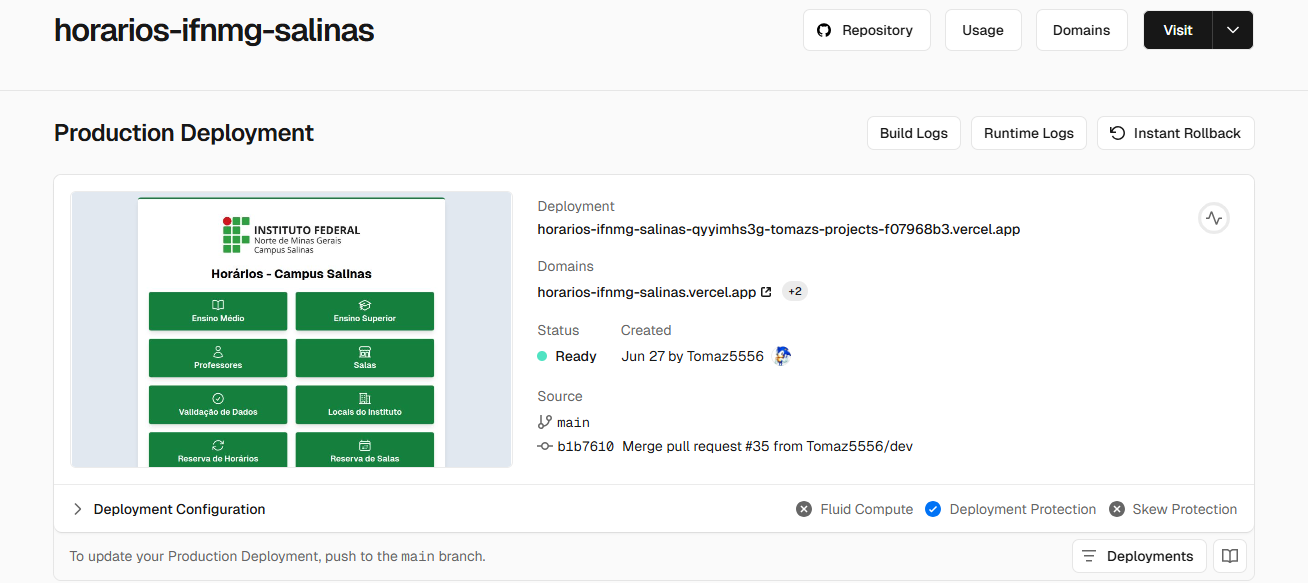
\includegraphics[width=1\textwidth]{Figuras/deploy-1.png}
    \caption*{Fonte: AUTOR (2025)}
    \label{fig_deploy_1}
\end{figure}

Já o back-end foi hospedado na plataforma Koyeb, responsável por executar a API que processa e envia os dados do Google Sheets ao front-end, conforme ilustrado na Figura \ref{fig_deploy_2}.

\begin{figure}[H]
    \centering
    \caption{Deploy do back-end da plataforma na Koyeb}
    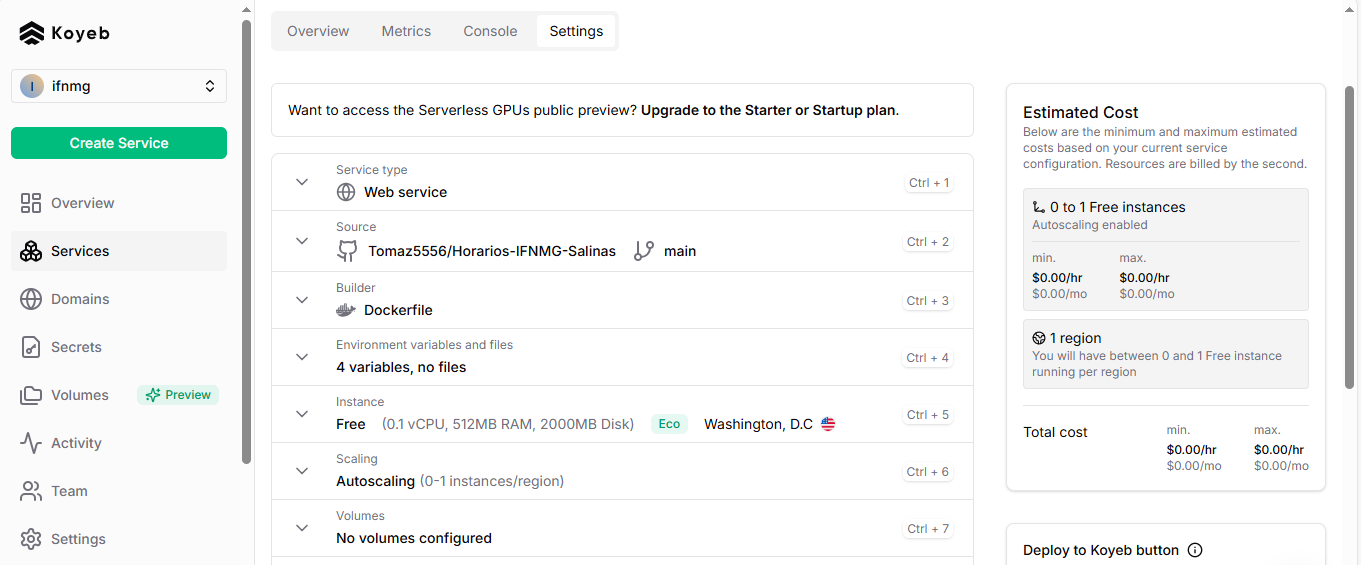
\includegraphics[width=1\textwidth]{Figuras/deploy-2.png}
    \caption*{Fonte: AUTOR (2025)}
    \label{fig_deploy_2}
\end{figure}

\section{Documentação}

As Figuras \ref{fig_doc_1}, \ref{fig_doc_2} e \ref{fig_doc_3} apresentam a documentação técnica elaborada para a planilha utilizada como banco de dados do sistema. A documentação está disponível no seguinte endereço \url{https://tomaz5556.github.io/Horarios-IFNMG-Salinas}. Esse material descreve, de forma clara e objetiva, as instruções para atualização do identificador da planilha, as regras de preenchimento dos dados, bem como os padrões de nomes e intervalos de células necessários para garantir a integridade do funcionamento da plataforma.

\begin{figure}[htb]
    \centering
    \caption{Instruções para desenvolvedores}
    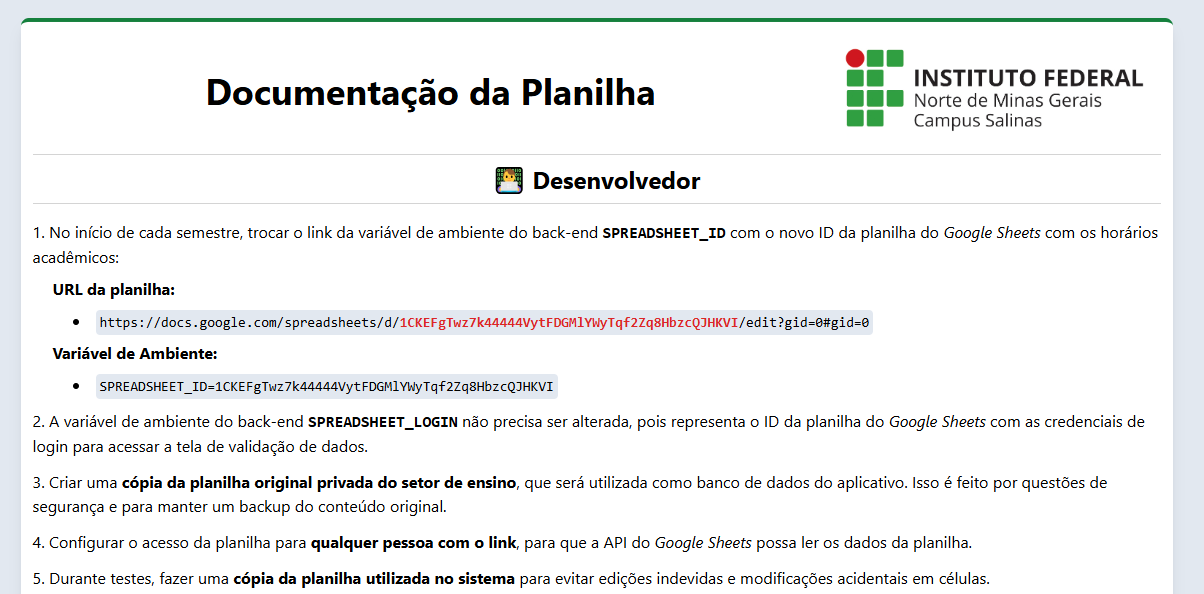
\includegraphics[width=0.9\textwidth]{Figuras/doc-1.png}
    \caption*{Fonte: AUTOR (2025)}
    \label{fig_doc_1}
\end{figure}

\begin{figure}[htb]
    \centering
    \caption{Instruções para administradores da planilha}
    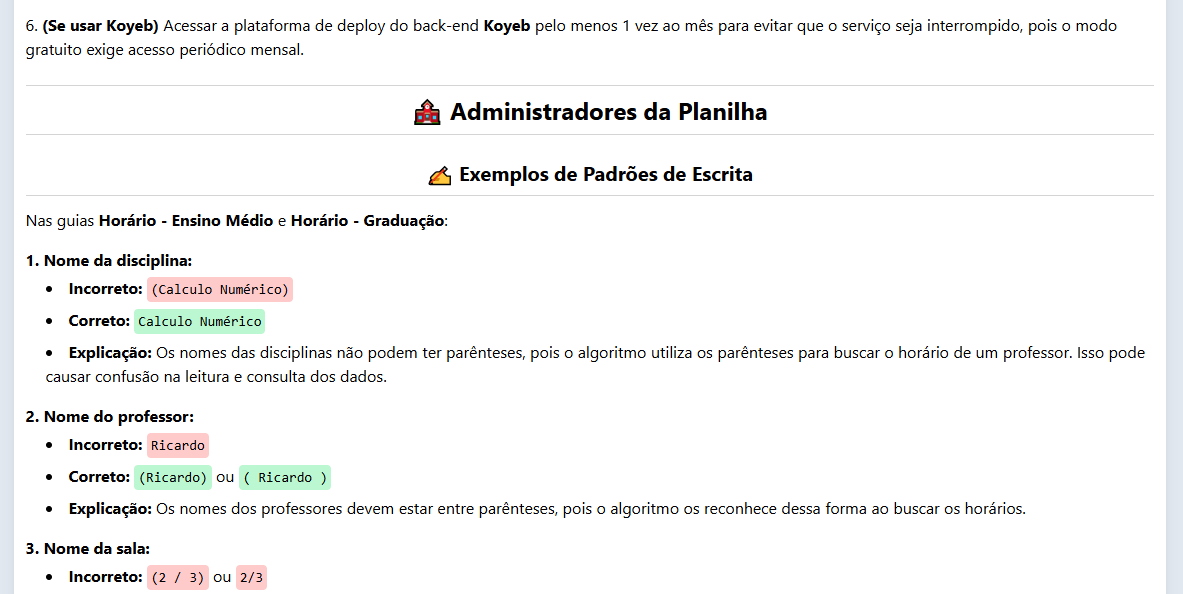
\includegraphics[width=0.9\textwidth]{Figuras/doc-2.png}
    \caption*{Fonte: AUTOR (2025)}
    \label{fig_doc_2}
\end{figure}

\begin{figure}[htb]
    \centering
    \caption{Explicação das guias e intervalos de células}
    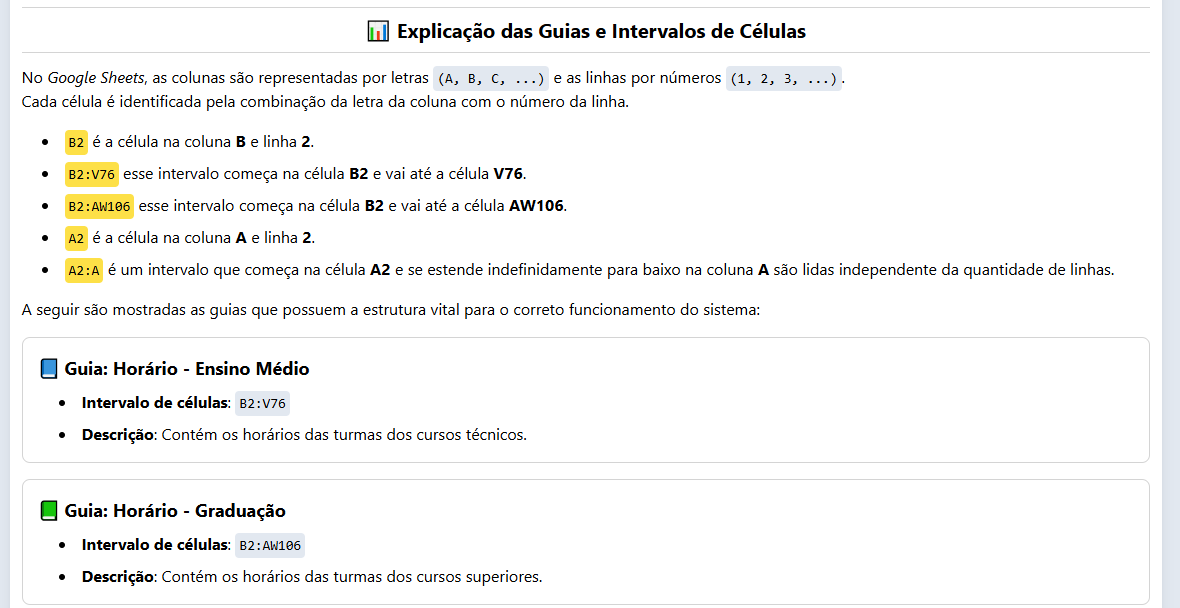
\includegraphics[width=0.9\textwidth]{Figuras/doc-3.png}
    \caption*{Fonte: AUTOR (2025)}
    \label{fig_doc_3}
\end{figure}

\begin{figure}[htb]
    \centering
    \caption{Observação sobre mudanças estruturais}
    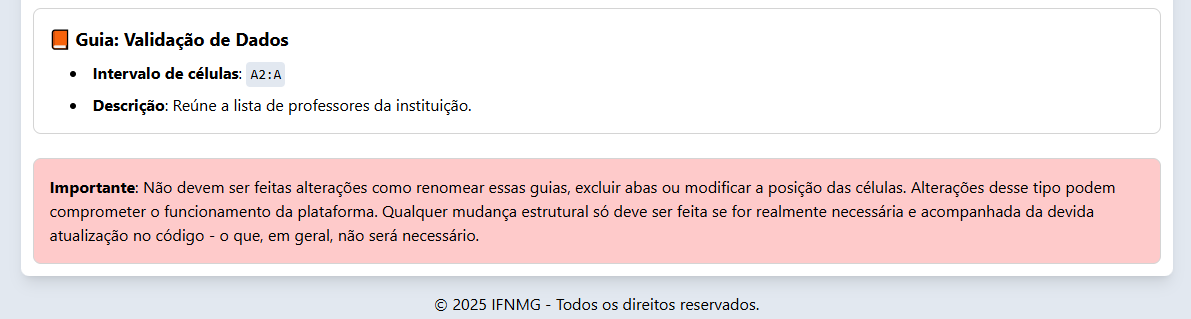
\includegraphics[width=0.9\textwidth]{Figuras/doc-4.png}
    \caption*{Fonte: AUTOR (2025)}
    \label{fig_doc_4}
\end{figure}
\chapter{Conclusão} 
\label{cap6_conclusao} 

O presente trabalho teve como foco facilitar a exibição dos horários acadêmicos do IFNMG - Campus Salinas, buscando tornar o acesso a essas informações mais intuitivo, seguro e eficiente, em resposta às demandas do setor de ensino. A pesquisa abordou a necessidade de modernização desse processo, considerando as limitações de usabilidade, segurança e organização presentes no modelo anterior baseado em planilhas no \textit{Google Sheets}. A solução proposta manteve as planilhas como base de dados, porém melhorou a forma de acesso, visualização e proteção dessas informações.

A relevância do trabalho se destaca por apresentar uma abordagem alternativa de banco de dados para sistemas web. A escolha dessa proposta refletiu uma necessidade real do setor de ensino da instituição e, ao mesmo tempo, representou um desafio técnico e prático que contribuiu significativamente para o desenvolvimento acadêmico e profissional.

Os objetivos foram alcançados. A plataforma foi desenvolvida com os conhecimentos obtidos durante o curso, avaliada por quem administra os horários acadêmicos e analisada quanto à sua viabilidade técnica. Além disso, foi elaborada uma documentação técnica da planilha utilizada como banco de dados, com diretrizes que orientam a manutenção e a continuidade do sistema, contribuindo diretamente para a melhoria do acesso e da organização dos horários acadêmicos da instituição.

Os resultados obtidos reforçam a efetividade da proposta, com a criação de telas específicas para cursos, professores e salas, além da implementação de uma tela de validação de dados com acesso restrito. A plataforma incorporou recursos de navegação mais claros e objetivos, sendo acompanhada de uma documentação técnica que assegura sua manutenção e continuidade. Tais melhorias contribuíram para aumentar a confiabilidade, acessibilidade e organização das informações, alinhando-se às demandas reais do setor de ensino.

Uma das principais dificuldades encontradas foi a escassez de materiais sobre o uso de planilhas como banco de dados em sistemas web, exigindo maior esforço de pesquisa e testes durante o desenvolvimento.

Por fim, como sugestão para trabalhos futuros, implementar uma funcionalidade que permita a edição dos horários diretamente pela interface da plataforma. Com essa melhoria, seria possível realizar modificações sem a necessidade de acessar as planilhas, contribuindo para otimizar o tempo de manutenção do sistema.

Para auxiliar o desenvolvimento de trabalhos futuros, o código-fonte da plataforma apresentada no trabalho está disponível em: \url{https://github.com/ifnmgsal-inf/Horarios-IFNMG-Salinas.git}.

%-----------------------------------
% Finaliza a parte no bookmark do PDF
% para que se inicie o bookmark na raiz
% e adiciona espaço de parte no Sumário
\phantompart

%-----------------------------------
% Bibliografia
\bibliography{referencias.bib}


%-----------------------------------
% POST-TEXTUAL ELEMENTS
%-----------------------------------
\postextual

% Apêndice
% Elemento opcional
%-----------------------------------
\begin{apendicesenv}
\label{apendice}
%-----------------------------------

%-----------------------------------
\chapter{Levantamento de Requisitos} \label{apendiceA}

\begin{figure}[htb] 
    \centering
    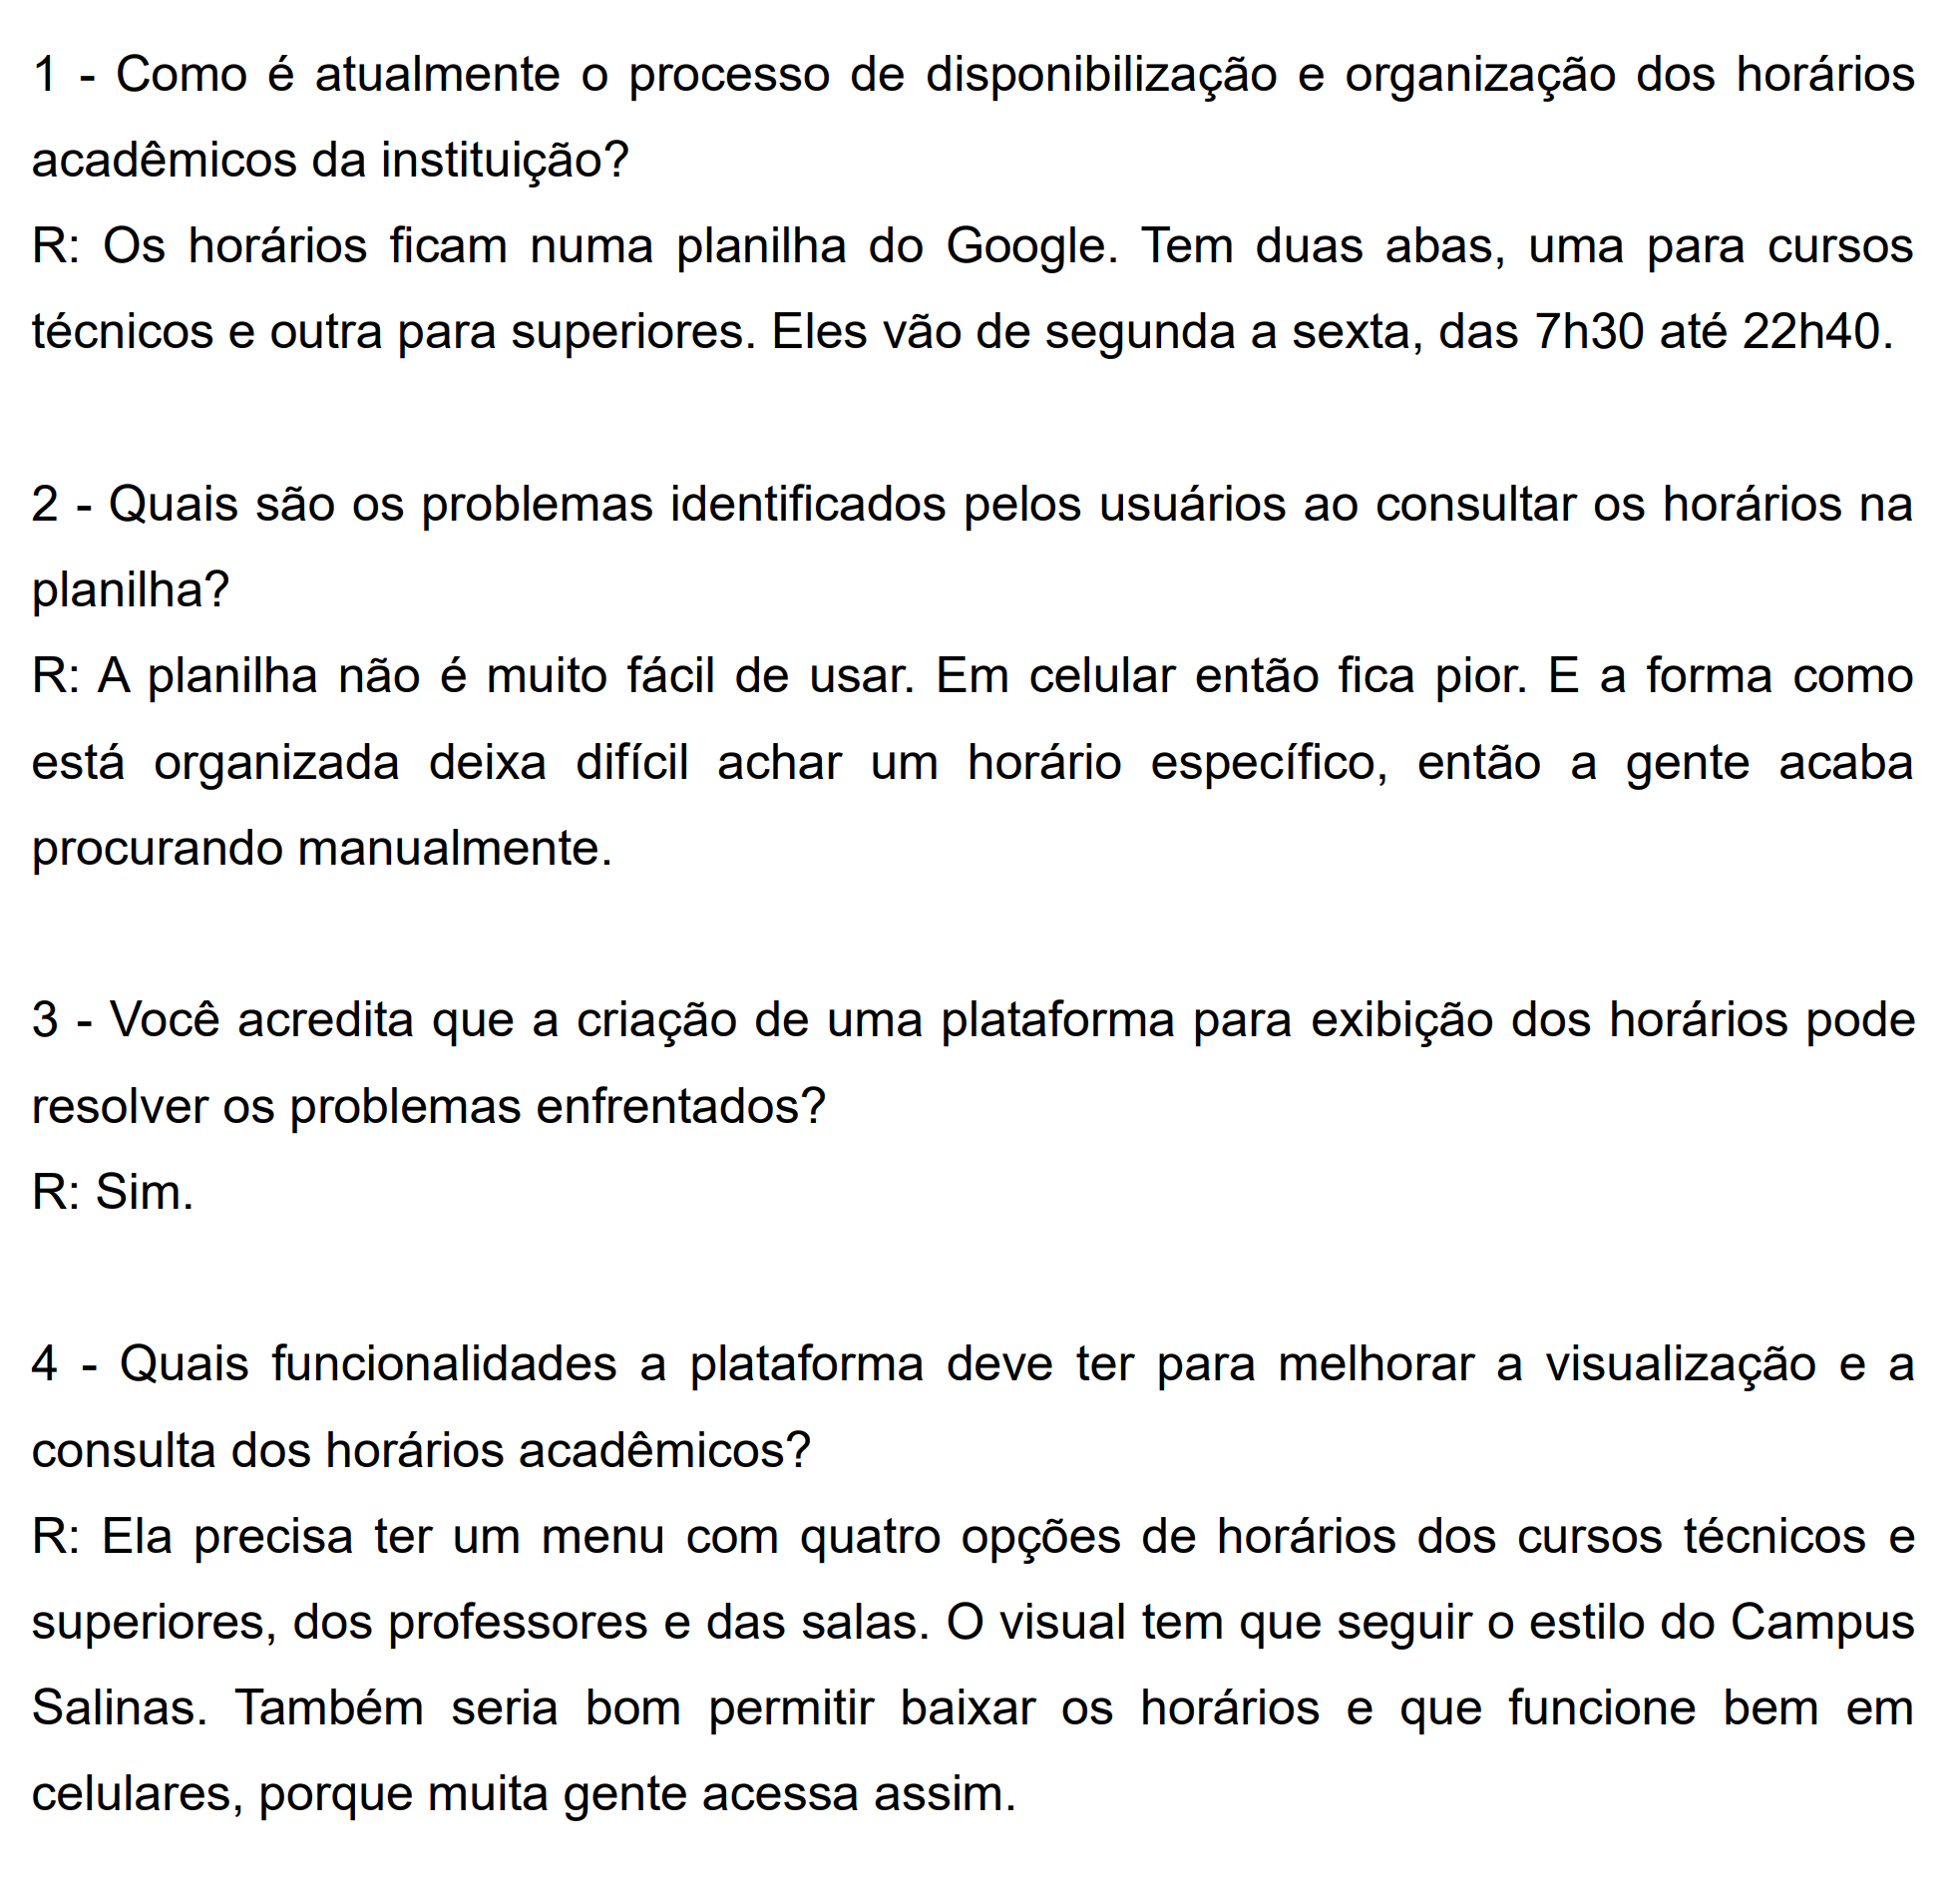
\includegraphics[width=1\textwidth]{Figuras/QLevantamento.png}
    \caption{Questionário de Levantamento de Requisitos}
    \label{fig_qlevantamento}
\end{figure}

\chapter{Avaliação da Plataforma} \label{apendiceB}

\begin{figure}[htb] 
    \centering
    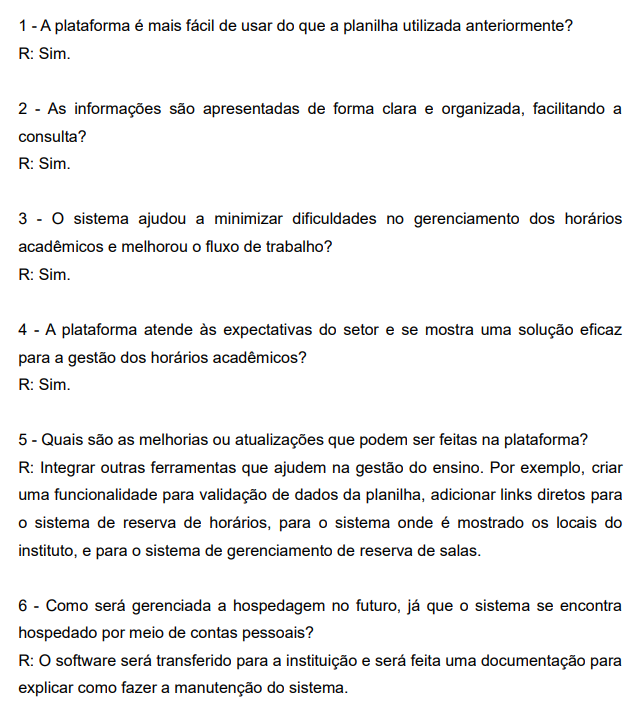
\includegraphics[width=1\textwidth]{Figuras/QAvaliacao.png}
    \caption{Questionário de Avaliação da Plataforma}
    \label{fig_qavaliacao}
\end{figure}

\end{apendicesenv}


\end{document}
